%!TEX root = ../my_thesis.tex
\section{Flavour tagging algorithms}
\label{sec:tagging}

In this chapter, a description of the \emph{flavour tagging} techniques at LHCb is reported.
After a brief introduction to the methods,
the calibration of the \emph{Opposite Side} (OS) and \emph{Same Side} (SS) algorithms for the $\Bz\to\Dpm\pimp$ 
time-dependent analysis are 
described. Finally, a reoptimisation of the OS \emph{electron} (\OSe) tagger on both Run 1 and Run 2 data is reported. 
This work was made in collaboration with the University of Dortmund. During my PhD work
activity, I focused mainly on the OS calibration and OSe reoptimisation.

The identification of the flavour at production time of a neutral $B$ meson, \ie~whether it contained a $\bquark$ or a $\bquarkbar$ quark at
production, is a key element 
for any time-dependent analysis aiming at the measurement of oscillations and \CP~asymmetries, and in particular for the $\Bz\to
\Dpm\pimp$ analysis reported in this thesis. In fact, this information is needed in order to measure the decay rates or asymmetries introduced in Sec.~\ref{sec:Bphysics}.
Complications arise from two facts:
\begin{itemize}[noitemsep,topsep=0pt]
	\item neutral $B$ meson oscillate, so the flavour at the production time might differ from the flavour at the decay time;
	\item there are many final states, such as $\Dmp\pipm$, that can be produced by the decay of both $B$ and $\bar B$ mesons; so, the flavour cannot be obtained from the charge of the final state, even if there were no oscillations.
\end{itemize}
For these reasons, the flavour has to be reconstructed by exploiting particles not produced in the decay of the neutral $B$ meson being analysed.

Techniques to infer the initial flavour of a reconstructed
candidate are called flavour tagging algorithms.
Several flavour tagging algorithms exist in LHCb; they can be categorised into
same-side taggers (SS taggers) and opposite-side taggers (OS taggers). A
schematic representation of the taggers that can be used for tagging $\Bz$
mesons is shown in Fig.~\ref{fig:FTscheme}.
\begin{figure}[t]
	\begin{center}
		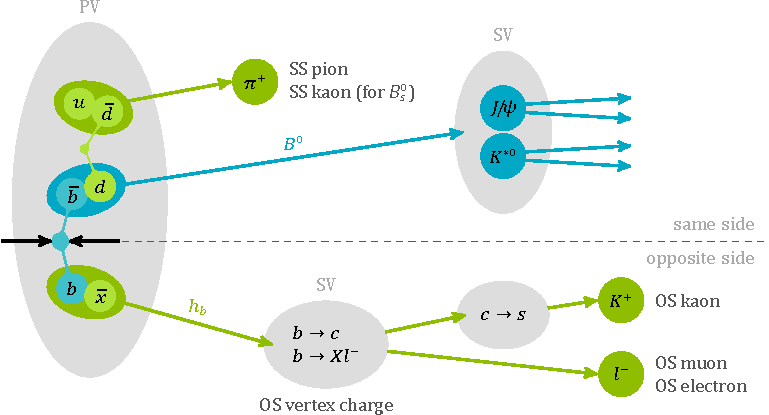
\includegraphics[width=0.8\textwidth]{04Flavourtagging/figs/FlavourTaggerScheme.pdf}
	\end{center}
        \vspace{-2mm}
	\caption{Flavour tagging algorithms used in LHCb. In this cartoon, the signal channel is considered to be $B^0\to J/\psi K^{*0}$.}
	\label{fig:FTscheme}
\end{figure}

The SS taggers infer the production flavour of the signal $\B$ meson by selecting
charged particle candidates that have a high chance of being remnants of the
hadronisation process of the $\B$ candidate
\cite{LHCb-PAPER-2016-039}. For $\Bz$ mesons, the same-side
pion tagger (\SSpi), which exploits charged $\pi$ mesons produced in the hadronisation of the
$\Bz$ meson, and the same-side proton tagger (\SSp), which looks for co-produced
protons, have been developed. For both taggers, the charge of the pion or proton is correlated with the production flavour of the signal $\Bz$ meson.
The response of the two taggers is combined into a
common SS response.

In contrast, the OS taggers exploit the predominant production process of $\B$
mesons via $\bbbar$ quark pair production \cite{LHCb-PAPER-2011-027}. They
partially reconstruct the decay of the \emph{other} $\bquark$ hadron produced along with each
reconstructed signal $\B$ meson, and infer its initial flavour. In fact, the flavour of the signal
$B$ meson and the other $\bquark$ hadron produced in the same collision are opposite.
Several OS taggers have been developed in LHCb, where the combination of the
OS kaon (\OSK), muon (\OSmu), electron (\OSe), and vertex charge (\OSvtx) tagging algorithms represents the
current standard OS combination. An additional OS tagger, the OS charm
tagger (\OSc)~\cite{LHCb-PAPER-2015-027}, can be exploited, and can be combined with
the OS standard combination.

Given a reconstructed candidate, each flavour tagging algorithm provides a
flavour tag $d$ and a prediction $\eta$ for the probability of the tag to be
wrong. This mistag probability $\eta$ is defined in the range $[0,0.5]$ and is
based on the output of multivariate classifiers, which are trained on datasets
of flavour-specific decays, and combine several kinematic and geometric
information on the tagging particle(s) and the event. The flavour tag takes the
values $d=+1$ for an initial $\Bz$, $d=-1$ for an initial $\Bzb$, and $d=0$ when
no tag could be assigned; this happens, for example, if the tagging particle fails 
the selection criteria of a given tagging algorithm, or if its trajectory lies outside
the detector acceptance.

More details on flavour tagging at LHCb can be found in
Refs.~\cite{Grabalosa:2012qra,LHCb-CONF-2011-003,LaThuile}.

%-------------------------------------------------------------------------------
\subsubsection{Performance characteristics}
\label{sec:tagging:characteristics}

The performance of flavour tagging algorithms can be characterised by different quantities. If $N_\mathrm{U}$ is the number of untagged
candidates and $N_\mathrm{W}$ ($N_\mathrm{R}$) is the number of wrongly (rightly) tagged candidates, the \emph{tagging efficiency}
(\ie~the fraction of tagged candidates) can be defined as
\begin{equation}
	\varepsilon_\text{tag}=\frac{N_\mathrm{R}+N_\mathrm{W}}{N_\mathrm{R}+N_\mathrm{W}+N_\mathrm{U}}.
	\label{eq:taggingefficiency}
\end{equation}
The fraction of wrongly tagged candidates, or \emph{mistag fraction}, is given by
\begin{equation}
\label{eq:mistag_def}
	\omega=\frac{N_\mathrm{W}}{N_\mathrm{R}+N_\mathrm{W}}.
\end{equation}
A non-zero mistag fraction dilutes the time-dependent asymmetries, reducing the experimental sensitivity to them. For instance, the measured decay rates for a $B\to f$ decay and its \CP-conjugate decay are
\begin{align}
	\frac{d\Gamma^{\rm meas}}{dt} &= (1-\omega)\frac{d\Gamma}{dt} + \omega \frac{d\bar\Gamma}{dt}, \\
	\frac{d\bar\Gamma^{\rm meas}}{dt} &= \omega\frac{d\Gamma}{dt} + (1-\omega) \frac{d\bar\Gamma}{dt}.
\end{align}
As a consequence, the measured \CP~asymmetry is
\begin{equation}
	A^{\rm meas}(t) = \frac{ \frac{d\bar\Gamma^{\rm meas}}{dt} - \frac{d\Gamma^{\rm meas}}{dt} }{ \frac{d\bar\Gamma^{\rm meas}}{dt} + \frac{d\Gamma^{\rm meas}}{dt} } 
	= \left(1-2\omega\right) \frac{ \frac{d\bar\Gamma}{dt} - \frac{d\Gamma}{dt} }{ \frac{d\bar\Gamma}{dt} + \frac{d\Gamma}{dt} } 
	= DA^{\rm phys}(t)\,, 
\end{equation}
where $A^{\rm phys}$ is the physical (true) \CP~asymmetry.
The quantity $D=1-2\omega$ is known as average \emph{dilution}. If $\omega=0$ (perfect tagger), then $D=1$ and no asymmetry dilution occurs. 
If $\omega=0.5$ (random tagger), then $D=0$, and it is not possible to measure the asymmetry anymore.

The quantity that can be interpreted as the figure of merit to
optimise a tagging algorithm is the
\emph{effective tagging efficiency}, also called \emph{tagging power}:
\begin{equation}
	\varepsilon_\text{eff}=\varepsilon_\text{tag}\left(1-2\omega\right)^2=\varepsilon_\text{tag}D^2.
\end{equation}
Assuming that $\varepsilon_\text{eff}$ is known without uncertainty, it can be shown that the statistical uncertainty on the physical asymmetry is given by
\begin{equation}
	\label{eq:sigma_on_asymm}
	\sigma_{A^{\rm phys}} = \frac{\sqrt{1-A^{\rm meas~2}}}{\sqrt{N\varepsilon_\text{tag}}\left(1-2\omega\right)}=\frac{\sqrt{1-A^{\rm meas~2}}}{\sqrt{N\varepsilon_\text{eff}}},
\end{equation}
where $N$ is the total number of candidates. So, according to Eq.~\ref{eq:sigma_on_asymm}, the greater the tagging power, the smaller the resulting statistical uncertainty on the \CP~asymmetry. 
Instead of using an average mistag fraction or \emph{probability} $\omega$, it is possible to exploit the
mistag probability $\eta$ estimated by the tagging algorithm. This probability $\eta$ is evaluated for each $B$ candidate individually, rather
than being a global quantity. Usually, $\eta$ needs to be \emph{calibrated} via a function $\omega(\eta)$ in order to return the true mistag probability (details in Sec.~\ref{sec:tagging:calibration}).
So, the tagging power can be rewritten as
\begin{equation}
	\label{eq:perevent_tagpower}
	\varepsilon_\text{eff} = \frac{1}{N}\sum_{i=1}^{N}D_i^2 = \frac{1}{N}\sum_{i=1}^{N}\left(1-2\omega(\eta_i)\right)^2,
\end{equation}
where $\omega(\eta_i)=0.5$ ($D_i=0$) for untagged candidates.

An example of dilution effect can be seen in Fig.~\ref{fig:dilution}, which shows how the measured amplitude of an asymmetry gets smaller for increasing values of $\eta$.

\begin{figure}[t]
	\begin{center}
		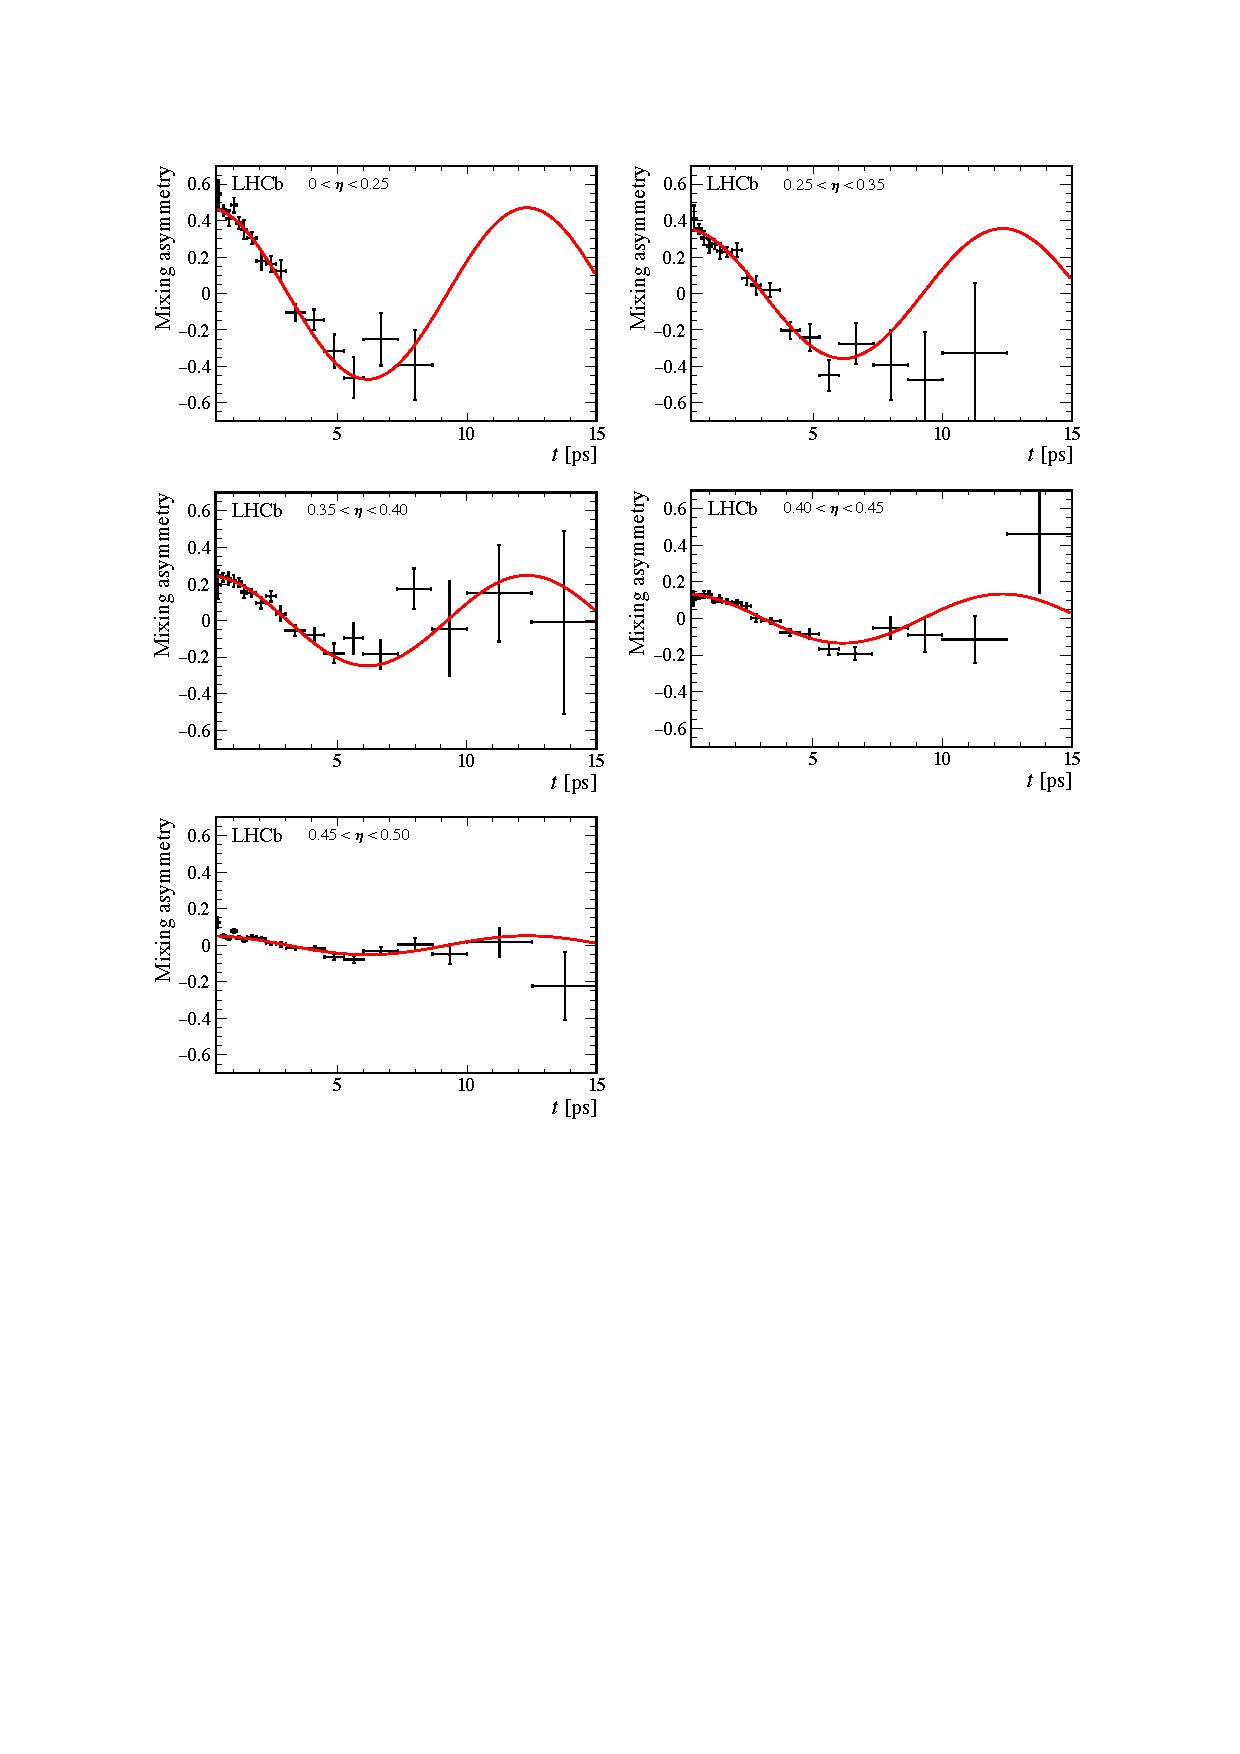
\includegraphics[width=0.9\textwidth]{04Flavourtagging/figs/Dilution.pdf}
	\end{center}
        \vspace{-2mm}
	\caption{Mixing asymmetry for SS-pion-tagged $B^0_s\to D^{\mp}_s\pi^{\pm}$ candidates in bins of increasing estimated mistag $\eta$~\cite{LHCb-PAPER-2016-039}.}
	\label{fig:dilution}
\end{figure}


%-------------------------------------------------------------------------------
\subsubsection{Calibration of the tagging output}
\label{sec:tagging:calibration}

The output of the flavour tagging algorithms is the result of training
multivariate classifiers (MVA) using datasets of flavour-specific $B$ decays, and
transforming the classifier output into mistag estimates $\eta$ through
regression. However, as the training and validation samples are different
from the signal sample used in the $\CP$ measurement (\eg~in terms of trigger
and selection criteria that affect the distribution of the MVA input features),
the output needs to be calibrated. Again, using control samples of flavour-specific decays, 
calibration functions $\omega(\eta)$ are obtained to
transform the mistag estimate $\eta$ of the algorithm to the mistag probability
$\omega$ measured in the control sample.

A common choice for the calibration function is a linear function:
\begin{equation}
	\omega(\eta)=p_0 + p_1\left(\eta-\langle\eta\rangle\right). \label{eq:FTcalibration}
\end{equation}
The use of the arithmetic mean $\langle\eta\rangle$ of the $\eta$ distribution
aims at a decorrelation of $p_0$ and $p_1$, hence a perfect calibration of the
taggers would result in $p_0=\langle\eta\rangle$ and $p_1=1$.

The performance of the flavour taggers is not necessarily independent of the
initial flavour of the \Bz. The charged decay products, like the \Kpm~mesons that are
used by the OS kaon tagger, can have significantly different interaction rates
with the detector material and therefore different reconstruction efficiencies.
This can result in different tagging efficiencies $\varepsilon_\text{tag}$ and
mistag probabilities $\omega$ for $\Bz$ and $\Bzb$. These tagging
asymmetries can dilute or enhance the observed raw asymmetry and need to be
corrected for. The asymmetries of the mistag probability, \ie~the difference of
the tagging calibration parameters $p_0$ and $p_1$ for initial $\Bz$ and $\Bzb$,
can be parameterised with two independent calibration functions:
\begin{equation}
	\begin{split}
          \label{eq:FTcalibrationSplit}
		\omega^{B^0}(\eta)  = p_0^{B^0}  + p_1^{B^0} \left(\eta-\langle\eta\rangle\right)\,,\\
		\omega^{\bar B^0}(\eta) = p_0^{\bar B^0} + p_1^{\bar B^0} \left(\eta-\langle\eta\rangle\right).
	\end{split}
\end{equation}
Equivalently, we can parameterise the calibration parameters $p_i$ (with $i=0,1$) as
\begin{equation}
	p_i^{B^0}=p_i+\frac{\Delta p_i}{2},\quad p_i^{\bar B^0}=p_i-\frac{\Delta p_i}{2}\,.
\end{equation}
The difference between the mistag of $\Bz$ and $\Bzb$ can be written as
\begin{equation}
		\Delta\omega(\eta)=\omega^{B^0}(\eta)-\omega^{\bar B^0}(\eta)=\Delta p_0+\Delta p_1\left(\eta-\langle\eta\rangle\right)\,.
\end{equation}

In this thesis, new models for the calibration functions are adopted instead
of the standard linear calibrations. These different parameterisations are
called \emph{Generalised Linear Models} (GLM), and are implemented in the EPM
(\emph{Espresso Performance Monitor}) package~\cite{EPM}. As will be explained in this section,
these models allow a great flexibility to cope with non-linearities, and solve technical issues
that may occur in fits that make use of flavour tagging. During my PhD, I worked
to refine some of these models and to include them in the fitting routines used for decay-time fits. 

In general, a GLM of order $N$ that relates the predicted mistag probability $\eta$ to the 
calibrated probability $\omega$ can be written as follows:
\begin{equation}
  \label{eq:glm_def}
  \omega(\eta) = g(h(\eta)) = g \left( g^{-1} (\eta) + \sum\limits_{i=1}^{N} \left(p_i + \frac{d\Delta p_i}{2}\right)f_i(\eta)\right)\,.
\end{equation}

The functions $f_i(\eta)$ are called \emph{basis functions}, and they can be chosen as polynomials or spline functions.
The set on basis functions is automatically orthogonalised by the EPM by using the Gram-Schmidt method~\cite{gram-schmidt}; this ensures that
the corresponding calibration parameters $p_i$ and $\Delta p_i$ are correlated as little as possible.

The parameter $d$ is the tagging decision, which is incorporated into the model in order to parameterise $\omega(\eta)$ for the two possible flavours.

The function $g$ is known as \emph{link function}. Usually, this is chosen as the inverse of a cumulative distribution
function in order to map input values into the interval $[0,1]$, such that the output can be naturally
interpreted as a probability.

For the $\Bz\to\Dpm\pimp$ analysis presented in this thesis, the adopted link function $g$ is a \emph{modified logistic function}, defined as
\begin{equation}
  \label{eq:rlogit}
  g(h) = \frac{1}{2(1+e^h)},
\end{equation}
where $h$ is defined in Eq.~\ref{eq:glm_def}. This link function is built such that the calibrated mistag probability
is defined in the interval $(0,0.5)$. This choice solves a numerical issue that often occurs when
standard link functions (\eg~identity or logistic) are adopted. In fact, if $\omega>0.5$, then an arbitrary
prescription has to be taken (\eg, label the candidate as untagged, or flip the tagging decision and take $1-\omega$ as
new calibrated mistag). If the calibration parameters are free in a time-dependent fit, this choice has to be made
during the minimisation process, according to the values $\omega$ takes at each iteration. This means that the relative
number of $B$ and $\bar B$, or the relative number of tagged and untagged candidates, may change during the fit, which
leads to numerical instabilities due to discontinuous changes in the likelihood function.

The EPM estimates the calibration parameters $p_i$ and $\Delta p_i$ via an unbinned maximum likelihood fit
called \emph{binomial regression}; this is an improvement over traditional, binned least-squares
fits, which are affected by a systematic uncertainty due to the binning choice.

%-------------------------------------------------------------------------------
\subsubsection{Combination of multiple taggers}
\label{sec:tagging:combination}

When more than one tagger is available per event, the tagging
decisions and mistag probabilities provided by each tagger can be combined into a single decision and a
single probability using the equations
\begin{equation}
	p(\bquark) = \prod_i\left(\frac{1}{2}-d_i\left(\frac{1}{2}-\eta_i\right)\right),\hspace{1cm}
	p(\bquarkbar) = \prod_i\left(\frac{1}{2}+d_i\left(\frac{1}{2}-\eta_i\right)\right), \label{eq:FTcombination1}
\end{equation}
where $p(\bquarkbar/\bquark)$ is the probability that the signal \Bz~contains a \bquarkbar/\bquark,
$d_i$ is the decision taken by the $i$-th tagger and
$\eta_i$ is the predicted mistag probability of the $i$-th tagger. These probabilities are
normalised as
\begin{equation}
	P(\bquarkbar) = \frac{p(\bquarkbar)}{p(\bquarkbar)+p(\bquark)}, \hspace{1cm} P(\bquark) = 1 - P(\bquarkbar). \label{eq:FTcombination2}
\end{equation}
If $P(\bquarkbar)>P(\bquark)$ the combined tagging decision is $d=+1$ and the final mistag probability is
$\eta = 1-P(\bquarkbar)$. Otherwise if $P(\bquark)>P(\bquarkbar)$ the combined tagging decision and the mistag
probability are $d=-1$ and $\eta=1-P(\bquark)$. 

Equation~\ref{eq:FTcombination1} is valid under the assumption that all taggers in the combination are independent.
In the $\Bz\to\Dpm\pimp$ analysis presented in this thesis, the OS taggers are combined in a single OS combination, and
the same is done for the SS taggers. Effects due to correlations among taggers within a combination are corrected for by calibrating
the combined predicted mistag.

%-------------------------------------------------------------------------------

\section[Flavour tagging strategy for the $\Bz\to\Dpm\pimp$ time-dependent analysis]{Flavour tagging strategy for the \boldmath{$\Bz\to\Dpm\pimp$} time-dependent analysis}
\label{sec:tagging:strategy}
In the $\Bz\to\Dpm\pimp$ analysis presented in this thesis, the OS combination (including the OS charm tagger) and the SS
combination are used. The implementation of the OS algorithms used in the combination are the same as described
in Refs.~\cite{LHCb-PAPER-2011-027,LHCb-PAPER-2015-027}; the OS algorithms other than the OS charm tagger were built as neural networks
trained on $\Bp\to J/\psi K^+$ Run 1 data, whereas the OS charm tagger was implemented with a BDT trained on a cocktail of simulated
$\Bp\to J/\psi K^+$, $\Bz\to\jpsi\Kstarz$ and $B^0_s\to J/\psi\phi$ decays.
The SS taggers have been reimplemented for this specific analysis by exploiting $\Bz\to\jpsi\Kstarz$ decays.
The functional form of the tagging calibrations is studied in control samples of
flavour-specific decays properly corrected to resemble the signal decay.
The calibration parameters are determined directly in the decay-time-dependent
fit of the signal described in Sec.~\ref{sec:datafit};
they are nuisance parameters of the likelihood function.
Determining the calibration parameters from the data along with
the \CP~observables is possible because the \CP~coefficients $C_f$ and $C_{\bar f}$ of Eqs.~\ref{eq:P0tof}--\ref{eq:P0bartofbar} are fixed in this analysis
(to \num{+1} and \num{-1} respectively). Hence, the cosine terms give sensitivity to the calibration parameters
independently of the sine terms, which are proportional to the $S_f$ and $S_{\bar{f}}$ coefficients. A heuristic explanation is presented in
Fig.~\ref{fig:amplitudes}.
\begin{figure}[t]
        \begin{center}
                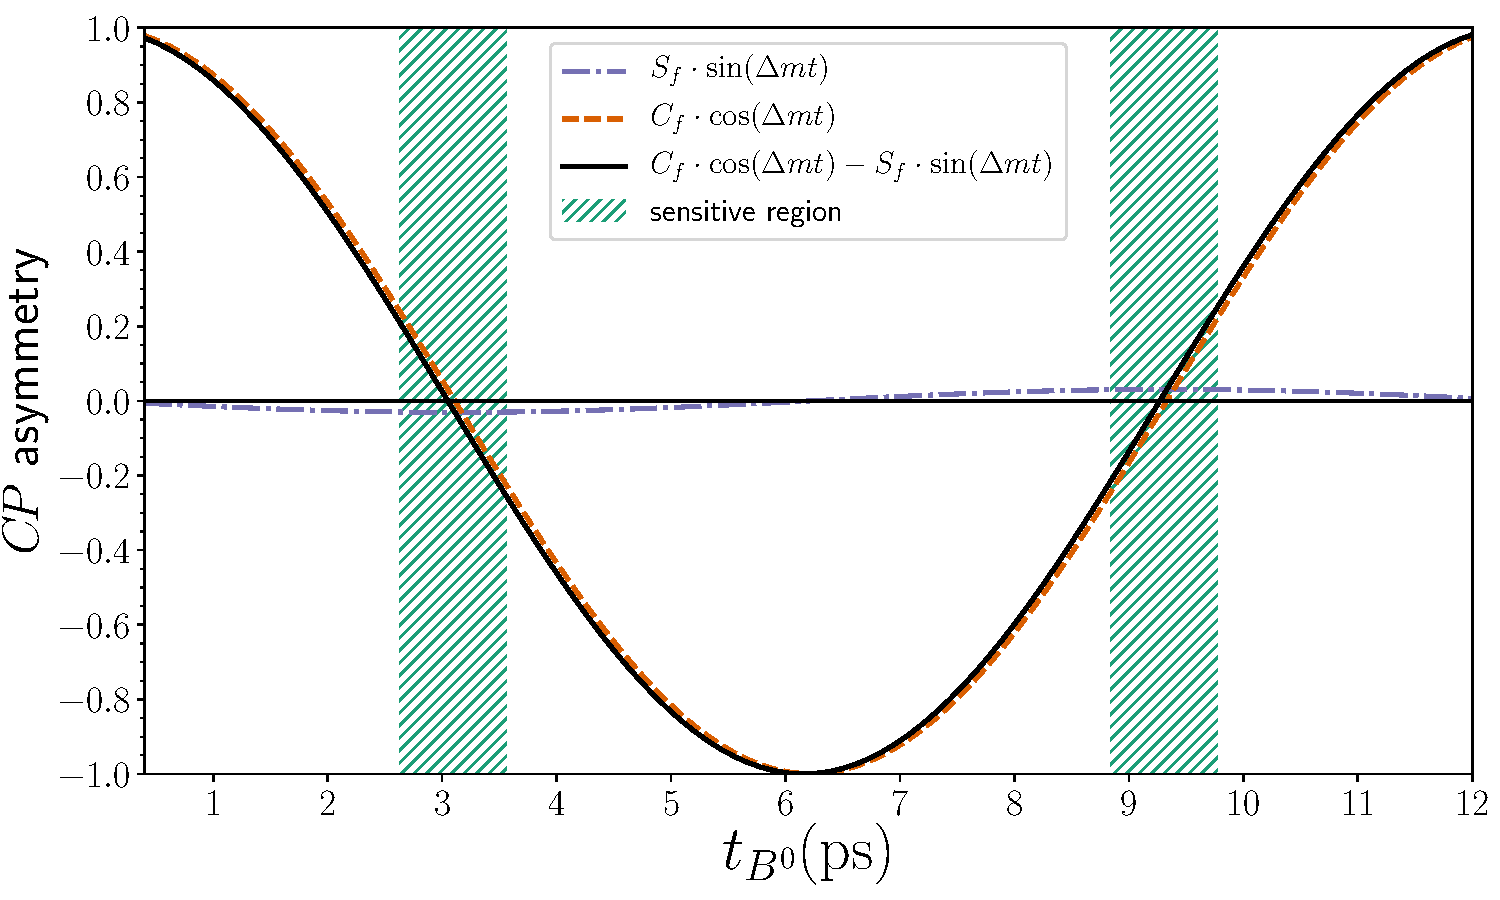
\includegraphics[width=0.48\linewidth]{04Flavourtagging/figs/oscillation_f.pdf}
                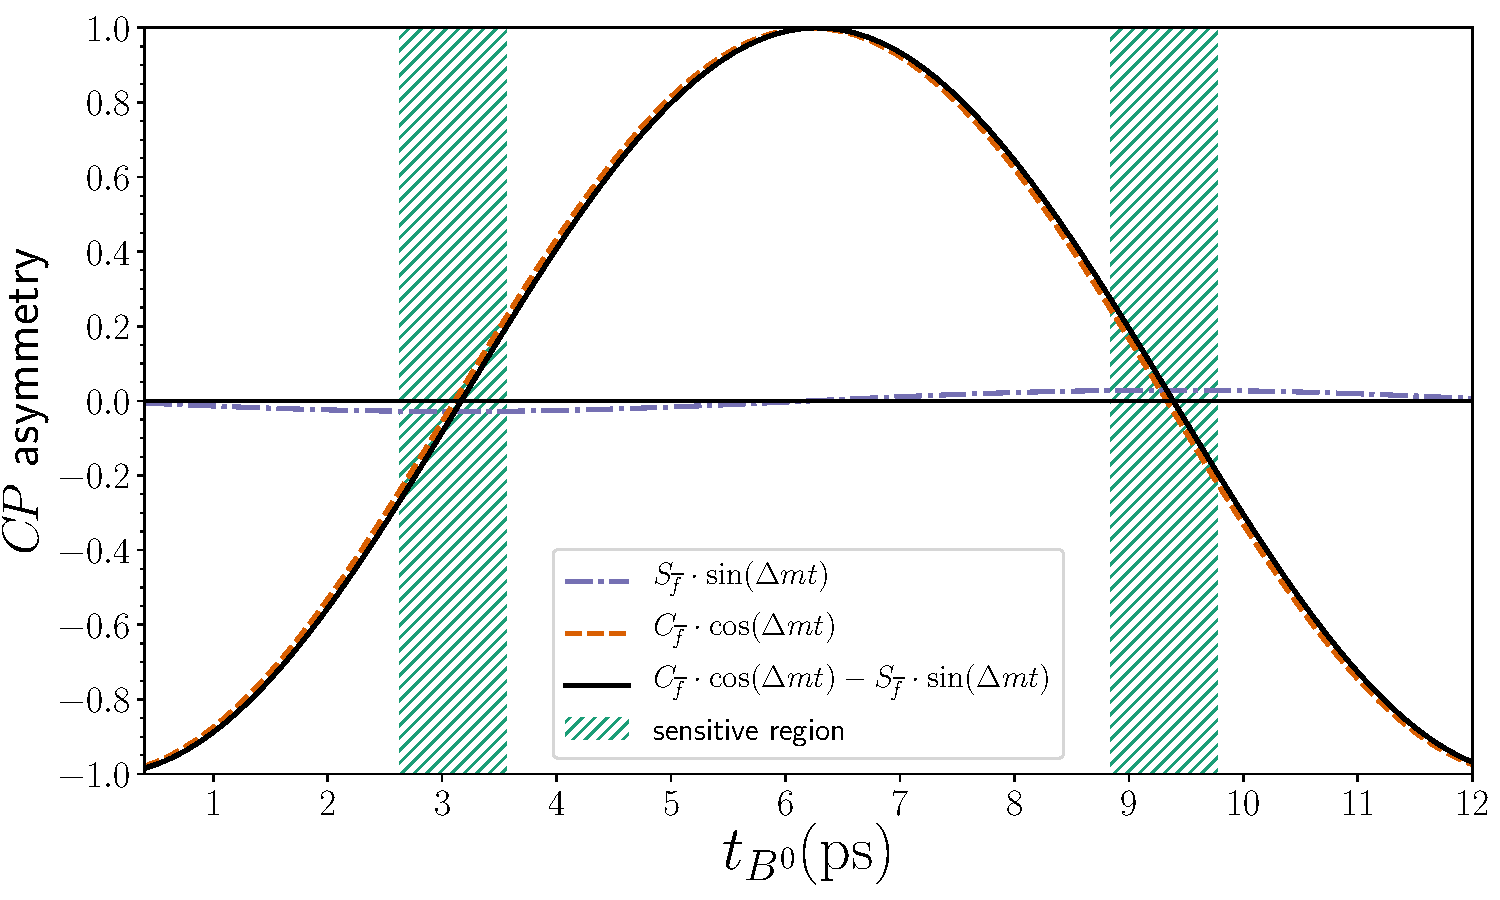
\includegraphics[width=0.48\linewidth]{04Flavourtagging/figs/oscillation_fbar.pdf}
        \end{center}
        \vspace{-2mm}
        \caption{$\bar\Bz$ versus $\Bz$ time-dependent asymmetries for the $\Dm\pip$ (left) and $\Dp\pim$
        (right) final states. The values of $C_f$, $C_{\bar f}$, $S_f$ and $S_{\bar f}$ are the ones used in simulation (see Appendix~\ref{app:mcgen}). 
        The sensitivity to $S_f$ and $S_{\bar f}$ is maximised in the
        intervals called ``sensitive regions'', since the $\sin(\Delta m)$ amplitude becomes of the same order of
        the $\cos(\Delta m)$ amplitude, which is close to zero. In the outer regions, since $C_f$ ($C_{\bar f}$) is
        fixed to $1$ ($-1$) in the fit, the mistag dilution (which depends on the flavour tagging calibration
        parameters) adapts to fit the $\cos(\Delta m)$ amplitude, giving sensitivity to the calibration parameters.}
        \label{fig:amplitudes}
\end{figure}
This strategy avoids any assumption on the portability
to the signal sample of the calibration parameters determined from the control
data. Such a strategy was studied extensively on simulation: the increase of the
statistical uncertainty of the $S_f$ and $S_{\bar{f}}$ coefficients given by the additional degrees of freedom of
the calibration parameters is smaller than the systematic
uncertainties associated with the calibration portability. Moreover,
the use of the calibration parameters from the control sample
causes biases on $S_f$ and $S_{\bar{f}}$ of the order of their statistical uncertainty; when letting
the calibration parameters float in the fit, such biases are suppressed or disappear, at the cost
of a moderate increase of the statistical uncertainty. In addition, while the precision
of the OS tagger calibration from the control sample is similar to the one from the
signal sample, the calibration of the SS tagger derived from the signal sample (Tab.~\ref{tab:timefitresult})
is much more precise than that from the control sample (Tab.~\ref{tab:calibrationSScombination}).

In what follows, the study of the tagging calibration from the control sample is presented.
For all reasons discussed above, these studies are not meant for determining the calibration parameters to use in
the time fit to the signal data (usual strategy adopted in all flavour-tagged time-dependent analyses), but they
serve the purpose of: i) determining the best functional form of the calibration functions to be used in the fit to
the signal; ii) having some reference values for the calibration parameters for a comparison with those extracted
from the signal.

The calibration for the OS combination are determined using $\Bp\to \Dz\pip$ decays, as
described in Sec.~\ref{sec:tagging:OScalib}. The SS pion and the SS proton taggers were developed
using $\Bz\to\Dmp\pipm$ data and assuming negligible $\CP$ violation.
The use of these algorithms in this analysis could bias the measurement.
Therefore, the SS taggers are retrained using $\Bz\to\jpsi\Kstarz$ decays. The calibration of the SS
combination is described in Sec.~\ref{sec:tagging:SScalib}.

%===============================================================================
\subsection{Calibration of the opposite-side tagger combination}
\label{sec:tagging:OScalib}

\subsubsection{Data sample selection}
\label{sec:tagging:OScalib:selection}

The calibration parameters of the OS tagger combination (namely the combination of
the OS electron, muon, kaon, vertex charge, and charm algorithms) are determined using $\Bp\to
\Dz(\to \Km\pip)\pip$ candidates reconstructed in $3\invfb$ of data.
Such a control decay mode provides very high statistics (more than 300k OS-tagged signal candidates) and
is very similar to the signal decay $\Bz\to\Dm\pip$.

Candidate $\Bp\to\Dz\pip$ decays are selected through the \spverb!B2D0PiD2HHBeauty2CharmLine! stripping line,
versions \spverb!S21r1! (2011 data) and \spverb!S21! (2012 data), of the \spverb!BhadronCompleteEvent! stream.
The $\Bp$ candidates are required to be TOS, \ie~to trigger on \\
\spverb!Hlt1TrackAllL0Decision! at the HLT1 stage,
and at least one among \\
\path{Hlt2Topo2BodyBBDTDecision},
\path{Hlt2Topo3BodyBBDTDecision}, and \\
\path{Hlt2Topo4BodyBBDTDecision} at HLT2.
The additional requirements listed in Table~\ref{tab:OSSelection} are applied to further
suppress backgrounds and enhance the signal purity.

A fit to the mass distribution of $\Bp$ candidates is done to calculate \emph{sWeights},
used in the subsequent steps of the analysis to subtract the backgrounds surviving the selection.
This fit is described in details in Appendix~\ref{app:OSmassFit}.

Event-by-event weights are calculated to equalise the $\Bp\to\Dz\pip$ and $\Bz\to\Dpm\pimp$ distributions of the variables on which
the tagging calibration can depend. The procedure and the results of this reweighting are reported in
Appendix~\ref{app:ReweightingOSTagging}. Additionally, the number of \Bp and \Bm candidates are made equal in the sample to avoid any spoil of the calibration
parameters due to a \Bp/\Bm production asymmetry or a detection asymmetry.
All these weights, along with \emph{sWeights}~\cite{Pivk:2004ty}, are applied during
the calibration procedure.

\begin{table}[htbp]
	\centering
	\caption{Selection requirements for the $\Bp\to\Dz\pip$ candidates.}
	\begin{tabular}{ccc}
		\toprule
		Description & Variable & Requirement \\
		\midrule
		\multicolumn{3}{c}{Bachelor track } \\
		\midrule
		muon identification criteria & $\text{IsMuon}$ & $=0$ \\
		ghost probability & $p_\text{ghost}$ & $<0.1$ \\
		quality of track & $\chi^2_\text{track}/\text{ndof}$ & $<2$ \\
		\midrule
		\multicolumn{3}{c}{$\Dz$ daughter tracks} \\
		\midrule
		$\ln L_K - \ln L_\pi$ & $\text{PIDK}$ & $>-2$ (kaon), $<8$ (pion) \\
		ghost probability & $p_\text{ghost}$ & $<0.1$ \\
		quality of track & $\chi^2_\text{track}/\text{ndof}$ & $<2.5$ \\
		\midrule
		\multicolumn{3}{c}{$\Dz$ candidate} \\
		\midrule
		invariant mass & $m_{K\pi}$ & $m_{K\pi}\in [1830,1904]~\mevcc$ \\	
		\midrule
                \multicolumn{3}{c}{$\Bp$ candidate} \\
		\midrule
		decay time & $\tau_{\Bp}$ & $\tau_{\Bp}\in [0.2,15]~\rm ps$ \\
		minimum IP $\chi^2$ w.r.t. PV & $\text{MIN}\chi^2\text{IP}_\text{PV}$ & $<15$ \\
		\bottomrule
	\end{tabular}
	\label{tab:OSSelection}
\end{table}

\subsubsection{Calibration}
\label{sec:tagging:OScalib:calibration}
The calibration of the estimated mistag $\eta$ is performed on the fully reweighted $\Bp\to\Dz\pip$ dataset. 
A GLM model with NSpline basis function~\cite{EPM} is adopted.
The projection of the fitted calibration function over the $\Bp\to\Dz\pip$ dataset is shown in Fig.~\ref{fig:oscalibplot},
whereas the fitted calibration parameters are listed in Table~\ref{tab:oscalibparams}.
\begin{figure}[htbp]
        \begin{center}
                \includegraphics[width=0.80\textwidth]{04Flavourtagging/figs/OS_Combination_Calibration_Data.png}
        \end{center}
        \vspace{-5mm}
        \caption{Mistag $\omega$ measured in bins of predicted mistag $\eta$ for reweighted $\Bp\to\Dz\pip$ candidates (data points) and fitted calibration function. The green (yellow) band indicates the $68\%$ ($95\%$) confidence interval on the calibration function.}
        \label{fig:oscalibplot}
\end{figure}
\begin{table}[htbp]
        \centering
        \caption{Fitted OS calibration parameters on the $\Bp\to\Dz\pip$ reweighted dataset.}
        \begin{tabular}{cc}
                \toprule
                Parameter & Fitted value \\
                \midrule
                $p_0$ & $-0.136 \pm 0.019$\\
                $p_1$ & $-0.006 \pm 0.022$\\
                $p_2$ & $-0.0107 \pm 0.0083$\\
                $p_3$ & $-0.5 \pm 0.10$\\
                $p_4$ & $-0.85 \pm 0.46$\\
                $\Delta p_0$ & $-0.129 \pm 0.038$\\
                $\Delta p_1$ & $0.042 \pm 0.045$\\
                $\Delta p_2$ & $-0.020 \pm 0.017$\\
                $\Delta p_3$ & $0.42 \pm 0.21$\\
                $\Delta p_4$ & $1.91 \pm 0.92$\\
                \bottomrule
        \end{tabular}
        \label{tab:oscalibparams}
\end{table}
The number of free parameters in the adopted GLM model (10) has been chosen in order to have  
satisfactory goodness-of-fit (GOF) metrics (details in Appendix~\ref{app:chooseOSdegree}).

\subsubsection{Calibration portability}
\label{sec:tagging:OScalib:portability}

The aim of the calibration is to return a mistag $\omega$ as close as possible to the \emph{true} mistag, which would
be given by a \emph{true calibration}. The latter is not defined for $\Bz\to\Dm\pip$ decays in data, but it is possible to estimate it 
for $\Bz\to\Dm\pip$ decays on MC. In fact, since the true flavour of the $\Bz$ meson
is known in MC, this true MC calibration can be done in the same way as $\Bp\to\Dz\pip$, where the true flavour is given by the $B$ charge.

This $\Bz\to\Dm\pip$ calibration is performed after equalising the number of $\Bz$ and $\bar\Bz$ in the sample, in order to disentangle
tagging asymmetries from \CP~violation and production asymmetries.

The $\Bp\to\Dz\pip$ MC calibration is performed in exactly the same way as described in Sec.~\ref{sec:tagging:OScalib:calibration}, except that no
\emph{sWeights} are considered, since only true MC signal decays are used.

The two calibrations using the $\Bz\to\Dm\pip$ and $\Bp\to\Dz\pip$ MC samples are shown in Fig.~\ref{fig:os_calib_portability_mc} and compared in Table~\ref{tab:os_calib_portability_mc}. A more robust comparison is obtained from a $\chi^2$ function describing the discrepancy between the two calibrations by taking the covariance matrices into account. The overall discrepancy (corresponding to the $\chi^2$ minimum) is around $2~\sigma$.

\begin{figure}[t!]
        \begin{center}
                \includegraphics[width=0.45\textwidth]{04Flavourtagging/figs/OS_Combination_Calibration_Bu_MC.png}
                \includegraphics[width=0.45\textwidth]{04Flavourtagging/figs/OS_Combination_Calibration_Bd_MC.png}
        \end{center}
        \vspace{-5mm}
        \caption{Mistag $\omega$ measured in bins of predicted mistag $\eta$ for reweighted $\Bp\to\Dz\pip$ (left) and $\Bz\to\Dm\pip$ (right) candidates (data points) and fitted calibration functions. The green (yellow) band indicates the $68\%$ ($95\%$) confidence interval on the calibration functions.}
        \label{fig:os_calib_portability_mc}
\end{figure}

\begin{table}[t!]
        \centering
        \caption{Comparison between the fitted OS tagging calibration parameters using truth-matched $\Bp\to\Dz\pip$ and $\Bz\to\Dm\pip$ MC decays. The discrepancy in each parameter is computed assuming independent datasets.}
        \begin{tabular}{cccc}
          \toprule
          Parameter   &  $\Bp\to\Dz\pip$   &  $\Bz\to\Dm\pip$  &   Discrepancy ($\sigma$) \\
          \midrule
          $p_0$   &   $-0.065\pm0.011$   &   $-0.0996\pm0.0066$   &   $2.70$ \\
          $p_1$   &   $-0.190\pm0.012$   &   $-0.1492\pm0.0077$   &   $-2.84$ \\
          $p_2$   &   $-0.0105\pm0.0044$   &   $-0.0191\pm0.0029$   &   $1.63$ \\
          $p_3$   &   $-0.295\pm0.054$   &   $-0.234\pm0.036$   &   $-0.93$ \\
          $p_4$   &   $-0.42\pm0.26$   &   $-0.14\pm0.20$   &   $-0.85$ \\
          $\Delta p_0$   &   $-0.059\pm0.022$   &   $-0.058\pm0.013$   &   $-0.03$ \\
          $\Delta p_1$   &   $0.044\pm0.024$   &   $0.030\pm0.015$   &   $0.46$ \\
          $\Delta p_2$   &   $-0.0012\pm0.0088$   &   $-0.0126\pm0.0058$   &   $1.08$ \\
          $\Delta p_3$   &   $-0.08\pm0.11$   &   $-0.046\pm0.073$   &   $-0.25$ \\
          $\Delta p_4$   &   $-0.34\pm0.53$   &   $-0.29\pm0.39$   &   $-0.08$ \\
          \bottomrule
        \end{tabular}
        \label{tab:os_calib_portability_mc}
\end{table}

%===============================================================================
\subsection{Calibration of the same-side tagger combination}
\label{sec:tagging:SScalib}

As described in Ref.~\cite{LHCb-PAPER-2016-039}, the SS pion and proton taggers
were both trained on the $\num{2012}$ data sample of
$\Bz\to\Dmp\pipm$ decays. As the effect of $\CP$ violation was neglected during the
training the algorithms and the underlying MVAs cannot be blindly used when
measuring $\CP$ violation in the same decay channel. Thus, $\Bz\to\jpsi\Kstarz$
decays are chosen instead, as they represent a flavour-specific $\Bz$ decay with
a large signal yield of about $350000$ candidates in 2012 data. 

Once the SS pion and proton taggers are implemented, they are combined into
a single SS combination as described in Sec.~\ref{sec:tagging:combination}.

%-------------------------------------------------------------------------------
\subsubsection{Calibration}
\label{sec:tagging:SScalib:combo}

The calibration is performed on a $\Bz\to\jpsi\Kstarz$ data subsample that is not used for the SS pion and proton training.
A GLM model having a first order polynomial is chosen as basis function and a
modified logistic function (Eq.~\ref{eq:rlogit}) is used as link. The number of free parameters in this model (4) is tuned in order to have
satisfactory goodness-of-fit (GOF) metrics. Together with the \emph{sWeights},
additional weights to correct the $\Bz\to\jpsi\Kstarz$ data to resemble the $\Bz\to\Dpm\pimp$ data are applied during the calibration. The
resulting calibration parameters are listed in Table~\ref{tab:calibrationSScombination} and a graphical representation of the calibration 
is presented in Fig.~\ref{fig:calibrationSScombination}.
\begin{table}[tbp]
	\centering
	\caption{Fitted SS calibration parameters obtained on the $\Bz\to\jpsi\Kstarz$ data sample (calibration
	subsample).}
	\begin{tabular}{cccc}
		\toprule
		$p_0$ & $p_1$ & $\Delta p_0$ & $\Delta p_1$ \\
		\midrule
		\num{-0.091\pm0.059}  & \num{-0.027\pm0.065} & \num{0.034\pm0.084} &\num{0.032\pm0.094}\\
		\bottomrule
	\end{tabular}
	\label{tab:calibrationSScombination}
\end{table}
\begin{figure}[tbp]
	\begin{center}
		\includegraphics[width=0.80\textwidth]{04Flavourtagging/figs/SScalib.png}
	\end{center}
        \vspace{-2mm}
	\caption{Mistag $\omega$ measured in bins of predicted mistag $\eta$ for reweighted $\Bz\to\jpsi\Kstarz$ candidates (data points) and fitted calibration function. The green (yellow) band indicates the $68\%$ ($95\%$) confidence interval on the calibration function.}	
	\label{fig:calibrationSScombination}
\end{figure}
%-------------------------------------------------------------------------------
\subsubsection{Calibration portability}
\label{sec:tagging:SScalib:portability}

In the same way as for the OS taggers (Sec.~\ref{sec:tagging:OScalib:portability}), the portability of the SS tagging calibration is checked on Monte Carlo. 
For $\Bz\to\Dm\pip$ the calibration is performed using the true flavour of the $\Bz$ meson after
equalising the number of $\Bz$ and $\bar\Bz$ in the sample, in order to disentangle tagging asymmetries from \CP~violation
and production asymmetries. Also on $\Bz\to\jpsi\Kstarz$ the true flavour of the $\Bz$ meson is used for the calibration, and
no \emph{sWeights} are needed, since only the true MC signal decays are used.

The two calibrations using the  $\Bz\to\Dm\pip$ and $\Bz\to\jpsi\Kstarz$ Monte Carlo samples are shown in
Fig.~\ref{fig:ss_calib_portability_mc} and compared in
Table~\ref{tab:ss_calib_portability_mc}. A full comparison that takes into account the correlation between the
parameters is obtained from a $\chi^2$ test similar to the one described in Sec.~\ref{sec:tagging:OScalib:portability}. The agreement is around \SI{0.1}{\sigma}. Even thought this test doesn't hint to
issues of portability between the decay modes, the same strategy used for the OS calibrations is followed, i.e fitting the
parameter directly in data with the \CP~asymmetries. This is motivated by the fact that 
the $\Bz\to\Dm\pip$ signal sample has much more sensitivity to determine the
parameters than the $\Bz\to\jpsi\Kstarz$ sample. In addition, with this approach no systematic related to calibration
portability is necessary, consistent with the OS tagger treatment.

\begin{figure}[t]
        \begin{center}
                \includegraphics[width=0.45\textwidth]{04Flavourtagging/figs/SS_Combination_Calibration_BdJpsiKst_MC.png}
                \includegraphics[width=0.45\textwidth]{04Flavourtagging/figs/SS_Combination_Calibration_BdDpi_MC.png}
        \end{center}
        \vspace{-2mm}
        \caption{Mistag $\omega$ measured in bins of predicted mistag $\eta$ for reweighted $\Bz\to\jpsi\Kstarz$ (left) and $\Bz\to\Dm\pip$ (right) candidates (data points) and fitted calibration functions. The green (yellow) band indicates the $68\%$ ($95\%$) confidence interval on the calibration functions.}
        \label{fig:ss_calib_portability_mc}
\end{figure}

\begin{table}[tbp]
        \centering
        \caption{Comparison between the fitted SS tagging calibration parameters using truth-matched \mbox{$\Bz\to\jpsi\Kstarz$} and $\Bz\to\Dm\pip$
        MC decays. The discrepancy in each parameter is computed assuming independent datasets.}
        \begin{tabular}{cccc}
          \toprule
          Parameter   &  $\Bz\to\jpsi\Kstarz$   &  $\Bz\to\Dm\pip$  &   Discrepancy ($\sigma$) \\
          \midrule
          $p_0$   &   $-0.016\pm0.017$   &   $-0.019\pm0.008$   &   $-0.19$ \\
          $p_1$   &   $0.063\pm0.021$   &   $0.060\pm0.010$   &   $-0.14$ \\
          $\Delta p_0$   &   $-0.029\pm0.033$   &   $-0.027\pm0.015$   &   $0.04$ \\
          $\Delta p_1$   &   $-0.026\pm0.041$   &   $0.015\pm0.019$   &   $0.90$ \\
          \bottomrule
        \end{tabular}
        \label{tab:ss_calib_portability_mc}
\end{table}

%===============================================================================
%!TEX root = ../my_thesis.tex
\section{Optimisation of the opposite-side electron tagger}
\label{sec:tagging:OSeOpt}

%%%%%%%%%%%%%%%%%%%%%%%%%%%%%%%%%%%%%%%%%%%%%%%%%%%%

The performance of the flavour tagging algorithms depends on the data taking conditions, in particular the centre-of-mass energy
of the $pp$ collision. 

On one hand, the tagging power of the SS taggers shows an increase on Run 2 data as compared to Run 1, thanks to either a higher tagging efficiency (\SSpi~and \SSp) or a lower mistag rate (\SSK). This is due to the higher boost of the $b\bar b$ quark pair at $13~\rm TeV$, which makes the momentum spectrum of $B$ mesons and fragmentation tracks harder, and increases the acceptance of the fragmentation tracks. 

On the other hand, the tagging power of the existing \OSe, \OSmu, and \OSK~taggers decreases on Run 2 data. The reason for this degradation is mainly due to the higher track multiplicity, which increases the probability to have a wrong tag decision. Moreover, because of the different Run 2 kinematics, the criteria to select the tagging particles are no longer optimal, thus giving a lower tagging efficiency.

The performance of the \OSc~and~\OSvtx~algorithms is, on average, compatible or better on Run 2 as compared to Run 1.

In this section, the reoptimisation of the \OSe~tagger is presented. This reoptimisation is performed both on Run 2 data, in order to recover the observed loss in tagging power, and on Run 1 data, to further improve the already existing algorithm.
This reoptimisation consists of two main steps. First, selection criteria are applied to select electron-like particles, yielding a sample of $B$ signal candidates with a low average tagging power. Then, a BDT classifier is applied to discriminate between $B$ candidates with right and wrong tag decisions for each selected track. Finally, for each $B$ candidate, the BDT output for the track with the highest transverse momentum is converted into a predicted mistag probability. 

A similar approach is followed for the development of the \OSK~and \OSmu~taggers. In this case, the reoptimisation on Run 1 data does not show any gain in performance, whereas some significant gain is found on Run 2 data.

%%%%%%%%%%%%%%%%%%%%%%%%%%%%%%%%%%%%%%%%%%%%%%%%%%%%

\subsection{Sample definition}

The \OSe~algorithm is developed in a data-driven fashion by using \emph{sWeighted} samples of $B^+\to J/\psi K^+$ decays. The full Run 1 dataset (2011+2012) is used to optimise the algorithm on Run 1 conditions, whereas the 2016 dataset is exploited to optimise the tagger on Run 2 conditions. An alternative optimisation on \emph{sWeighted} 2016 $B^+\to \Dzb \pi^+$ data is performed in parallel. The motivation for this is to cross-check the Run 2 implementation with an independent decay mode, which is characterised by different kinematics than that of $B^+\to J/\psi K^+$.
Hereafter, the \OSe~tagger optimised on Run 1 $B^+\to J/\psi K^+$ data will be indicated as ``Run 1 new'' version, in order to distinguish it from the previous ``Run 1 old'' version introduced in Ref.~\cite{LHCb-PAPER-2011-027}, which was based on simple selection criteria and a neural network for the mistag estimation.  
The \OSe~tagger optimised on Run 2 $B^+\to J/\psi K^+$ and $B^+\to \Dzb \pi^+$ data will be denoted as ``Run 2 B2CC'' and ``Run 2 B2OC'' versions, respectively.
Moreover, it is understood that the tunings of all the PROBNN features mentioned in this section are \texttt{MC12TuneV2} for Run 1 data and \texttt{MC15TuneV1} for Run 2 data.

Each dataset is divided in four subsamples:
\begin{itemize}[noitemsep,topsep=0pt]
  \item the first subset, including $\sim 25~\%$ of the total data, is used for the optimisation of the electron preselection (Sec.~\ref{sec:tagging:OSePresel});
    \item the second subset (\emph{training sample}), including $\sim 50~\%$ of the total data, is adopted as training set for the BDT classifier used for\
 the predicted mistag estimation (Sec.~\ref{sec:tagging:OSeBDT}). This sample is also used for tuning some \emph{hyperparameters} (number of trees, maximum depth) which define the BDT classifier.
 \item the third and the fourth subsets (\emph{evaluation set 1} and \emph{2}), each including $\sim 12.5~\%$ of the total data, are adopted together \
as test sets to check for overtraining (Sec.~\ref{sec:tagging:OSePerf1}). The evaluation set 1 is also used to calibrate the obtained tagger, which is then applied to the second evaluation set in order to measure the performance; the procedure is then repeated by swapping the two samples (\emph{two-fold validation}).
\end{itemize}

%%%%%%%%%%%%%%%%%%%%%%%%%%%%%%%%%%%%%%%%%%%%%%%%%%%%

\subsection{Preselection optimisation}
\label{sec:tagging:OSePresel}

Electron-like particles are selected by means of a set of requirements. The reconstructed tracks must not be associated to
the $B$ signal decay tree,
and must not have hits in the muon detector in order to exclude muons (already exploited by the \OSmu~algorithm).
Moreover, these tracks have to be of type long, lie in the ECAL acceptance, and have sufficient reconstruction quality ($\chi^2/\rm ndof<3$). 
Also, the inverse of the rigidity $e/p$ has to be comprised between 0.85 and 2, and the charge deposited in the VELO detector must be
smaller than 1.4 normalised Analogic-to-Digital Converter (ADC) counts.
Finally, tracks where the fit for the track IP with respect to the primary vertex did not converge are excluded. 

A further selection is applied in order to enhance the average tagging power of the resulting sample, which is defined as
\begin{equation}
        \label{eq:avgtagpower}
        \avg{\effeff} = \varepsilon_\text{tag} \left[1 - 2 \frac{\sum\limits_{i=1}^N w_i f^i_{\rm R}}{\sum\limits_{i=1}^N w_i (f^i_{\rm R} + f^i_{\rm W})}\right]^2,
\end{equation}
where $w_i$ are the \emph{sWeights}, while $f^i_{\rm R}$ ($f^i_{\rm W}$) is the fraction of particles giving the right (wrong) flavour for the $i$th $B$ candidate, with $f^i_{\rm R}+f^i_{\rm W}=1$ for every candidate.

The expression of Eq.~\ref{eq:avgtagpower} is taken as the figure of merit to maximise during the selection optimisation. This maximisation is performed numerically by using gradient boosted regression trees to model $\avg{\effeff}$ as a function of the applied cuts~\cite{scikit-optimize}. The cuts are optimised separately for the Run 1 new, Run 2 B2CC and Run 2 B2OC algorithms; in all cases, about $25\%$ of the available data for each sample is used. 

The resulting, optimised requirements are reported in Table~\ref{tab:OSegbselection}, while the convergence plots of the minimisation are shown in Fig.~\ref{fig:OSegbconvergence}.

After the optimisation, the performance of the selection (including the average tagging power defined in Eq.~\ref{eq:avgtagpower}) is evaluated on the remaining $75\%$ of data for each sample, yielding the results shown in Table~\ref{tab:OSegbperformance}.

\begin{table}
	\centering
        \caption{Optimised requirements for the preselection of tracks used by the \OSe~algorithm.
          $p_{\rm ghost}$ is the probability for the track to be a fake combination of hits.
          IPPU denotes the impact parameter with respect to the pile-up vertex in the event, which might be
        reconstructed in the event in addition to the nominal PV.
        $\Delta\phi$ is the difference in azimuthal angle between the track and the signal $B$ candidate.}
         \label{tab:OSegbselection}
        \begin{tabular}{llll}
        \toprule
        Requirement & Run 1 new & Run 2 B2CC & Run 2 B2OC \\
        \midrule
        $p_{\rm ghost}<$ & $0.861$ & $0.843$ & $0.348$ \\
        PROBNN$\pi<$ & $0.934$ & $0.983$ & $0.980$ \\
        PROBNN$p<$ & $0.719$ & $0.271$ & $0.732$\\
        PROBNN$K<$ & $0.765$ & $0.695$ & $0.954$\\
        PROBNN$e>$ & $0.061$ & $0.243$ & $0.040$\\
        PROBNN$\mu<$ & $0.938$ & $0.158$ & $0.263$ \\
        PID$e>$ & $4.555$ & $4.333$ & $-0.691$\\
        $p_{\rm T}>$ (\mevc) & $1132$ & $1403$ & $1263$ \\
        $p>$ (\mev) & $3114$ & $5035$ & $2246$\\
        $\sigma_{\rm IP}/\rm IP>$ & $0.020$ & $0.042$ & $1.410$ \\
        $\sigma_{\rm IPPU}/\rm IPPU>$ & $12.101$ & $9.335$ & $2.758$ \\
        min $\Delta\phi>$ & $0.00803$ & $0.0167$ & $0.0299$\\   
        \bottomrule
        \end{tabular}
\end{table}

\begin{table}
	\centering
        \caption{Performance of the preselection (\OSe~algorithm) applied on the data not used for the preselection optimisation ($\sim 75\%$ of the total dataset for each sample). The average tagging power $\avg{\effeff}$ is defined in Eq.~\ref{eq:avgtagpower}.}
        \label{tab:OSegbperformance}
        \begin{tabular}{llll}
        \toprule
        Algorithm & $\etag$ (\%) & $\avg{\mistag}$ (\%) & $\avg{\effeff}$ (\%) \\
        \midrule
        Run 1 new & $3.440\pm0.019$ & $33.31\pm0.27$ & $0.383\pm0.007$ \\
        Run 2 B2CC & $2.514\pm0.017$ & $33.50\pm0.32$ & $0.274\pm0.006$ \\
        Run 2 B2OC & $3.664\pm0.024$ & $34.32\pm0.32$ & $0.360\pm0.006$ \\
        \bottomrule
        \end{tabular}
\end{table}

\begin{figure}[htbp]
	\begin{center}
        \includegraphics[width=0.4\textwidth]{04Flavourtagging/figs/OSelectronOpt/2017-12-12-vibattis-OSElectron-tagpartseloptimisation_Run1/ConvergenceOSe2017-nominal.pdf}
        \includegraphics[width=0.4\textwidth]{04Flavourtagging/figs/OSelectronOpt/2017-12-12-vibattis-OSElectron-tagpartseloptimisation_Run2/ConvergenceOSe2017-nominal.pdf} \\
        \includegraphics[width=0.4\textwidth]{04Flavourtagging/figs/OSelectronOpt/2018-04-06-vibattis-OSElectron-tagpartseloptimisation_Run2_Bu2D0pi/ConvergenceOSe2017-nominal.pdf} \\
       \end{center}
        \vspace{-2mm}
        \caption{Maximised value of the average tagging power as a function of the gradient boosted regression tree algorithm iteration for the Run 1 new (top left), Run 2 B2CC (top right) and Run 2 B2OC (bottom) implementations of the \OSe~tagger.}
        \label{fig:OSegbconvergence}
\end{figure}

%%%%%%%%%%%%%%%%%%%%%%%%%%%%%%%%%%%%%%%%%%%%%%%%%%%%

\subsection{BDT classifier implementation}
\label{sec:tagging:OSeBDT}

The selection described in Sec.~\ref{sec:tagging:OSePresel} is applied on the remaining part of the data ($\sim 75~\%$) used by each \OSe~implementation.
The BDT classifier is trained to identify $B$ candidates as correctly or incorrectly tagged. The list of the features considered to build the BDTs are reported in Table~\ref{tab:OSefeatureslist}. The distributions of the input features for the two possible values of the target are shown in Figs.~\ref{fig:OSefeaturesRunI},~\ref{fig:OSefeaturesRunIIB2CC} and~\ref{fig:OSefeaturesRunIIB2OC} for the Run 1 new, Run 2 B2CC and Run 2 B2OC samples, respectively. The Pearson correlation coefficients between the input features are reported in Fig.~\ref{fig:OSecorrelations}.

\begin{table}
	\centering
        \caption{Features considered for the BDT used to evaluate the predicted mistag of the \OSe~tagger. For each tuning (Run 1 new, Run 2 B2CC and Run 2 B2OC), the symbol \cmark (\xmark) indicates
        if a given feature is included (discarded).}
         \label{tab:OSefeatureslist}
        %\resizebox{\textwidth}{!}{
        \begin{tabular*}{\textwidth}{@{}lcccc}
        \toprule
        Feature & Description & \begin{tabular}{c} Run 1 \\ new \end{tabular} & \begin{tabular}{c} Run 2 \\ B2CC \end{tabular} & \begin{tabular}{c} Run 2 \\ B2OC \end{tabular} \\
        \midrule
        nTracks & Number of reconstructed tracks & \cmark & \cmark & \cmark \\
        $p_{\rm T}$ & Transverse momentum of tagging track & \cmark & \cmark & \cmark \\
        $\sigma_{\rm IP}$ & IP uncertainty of tagging track & \cmark & \cmark & \cmark\\
        Signal $p_{\rm T}$ & Transverse momentum of $B$ candidate & \cmark & \cmark & \cmark\\
        BPV IP $\chi^2$ & IP $\chi^2$ of tagging track w.r.t $B$ vertex & \cmark & \cmark & \cmark\\
        $p_{\rm ghost}$ & Ghost probability & \cmark & \xmark & \cmark\\
        $e/p$ & Inverse rigidity & \cmark & \cmark & \cmark\\
        $\Delta r$ & \begin{tabular}{c} difference in $r$ coordinate \\ between $B$ and tagging track \end{tabular} & \cmark & \cmark & \cmark\\
        $|\rm IP|$ & Absolute value of tagging track IP & \cmark & \cmark & \cmark\\
        $\sigma_{\rm IPPU}/\rm IPPU$ & \begin{tabular}{c} Significance of the IP \\ w.r.t pile-up vertex for tagging track \end{tabular} & \cmark & \cmark & \cmark\\
        PROBNNg & Ghost probability from neural networks & \xmark & \cmark & \xmark \\
        $\Delta\eta$ & \begin{tabular}{c} Difference in pseudorapidity \\ between $B$ and tagging track \end{tabular} & \xmark & \cmark & \cmark \\
        $\Delta Q$ & \begin{tabular}{c} Magnitude of difference in momenta \\ between $B$ and tagging track \end{tabular} & \xmark & \cmark & \cmark\\
        \bottomrule
        \end{tabular*}
        %}
\end{table}

\begin{figure}[htbp]
        \begin{center}
        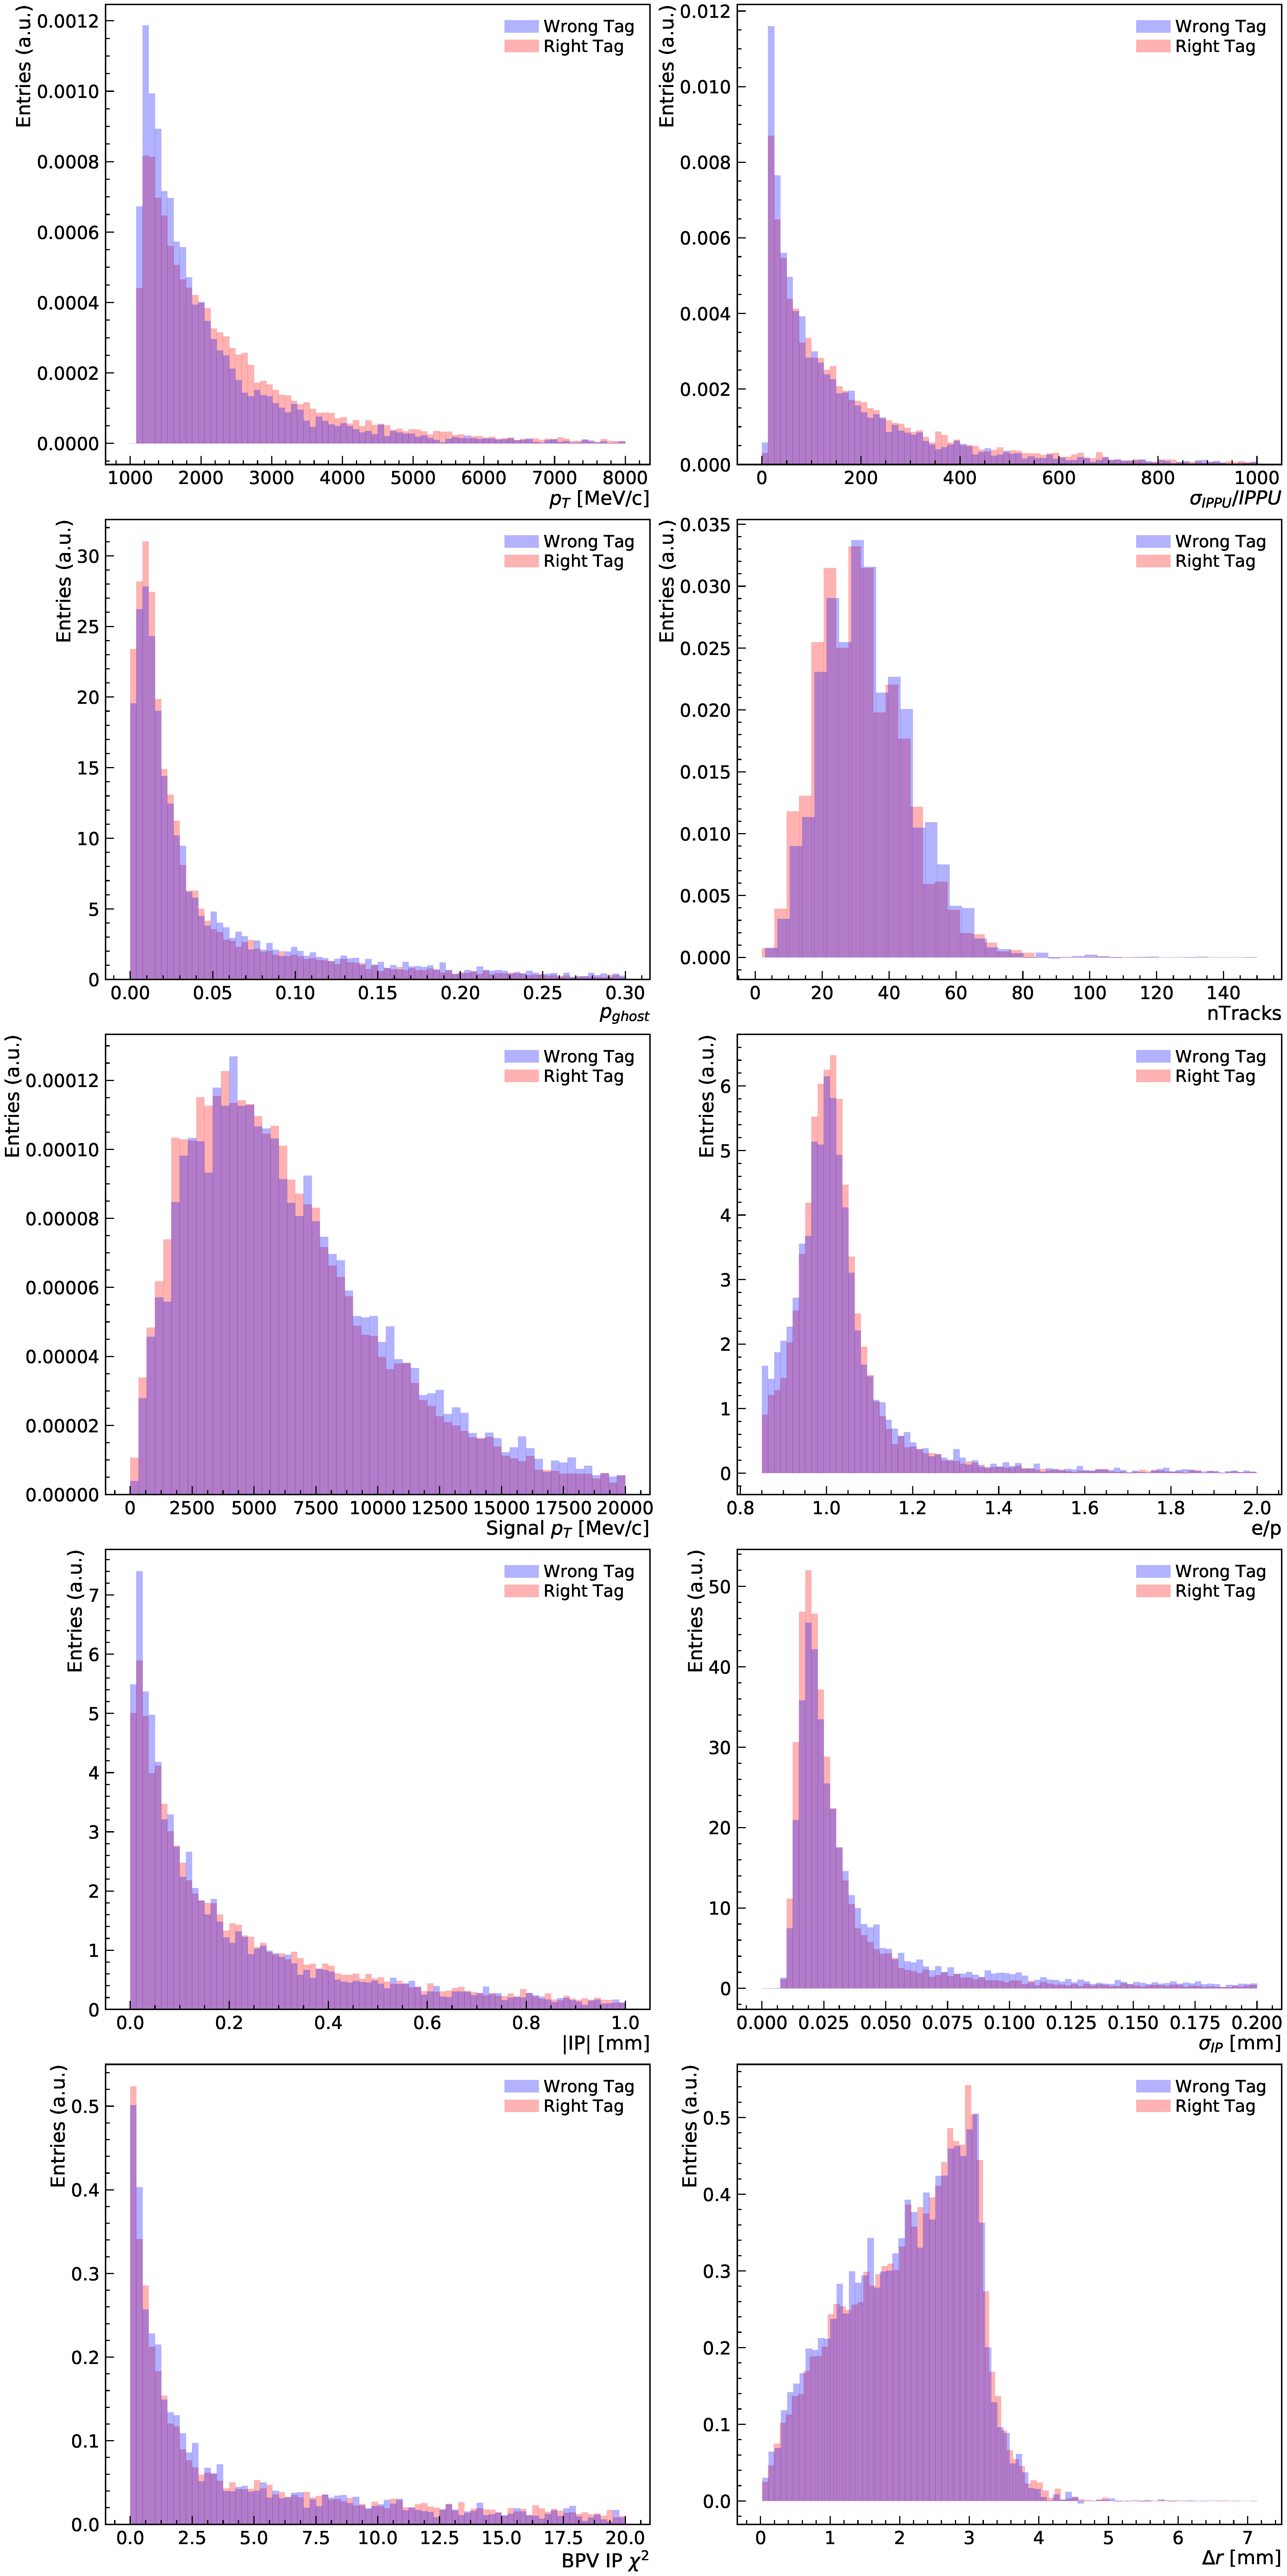
\includegraphics[width=0.7\textwidth]{04Flavourtagging/figs/OSelectronOpt/2017-12-12-vibattis-OSElectron-bdt-calibration-sWeights_Run1/FeaturesDistribution_RunIcuts.pdf}
        \end{center}
        \vspace{-2mm}
        \caption{Distributions (for the \emph{sWeighted}, Run 1 $B^+\to J/\psi K^+$ sample) of the input features of the BDT classifier, for candidates with a right (red) and wrong (blue) decision from the \OSe~tagger.}
         \label{fig:OSefeaturesRunI}
\end{figure}

\begin{figure}[htbp]
        \begin{center}
        \includegraphics[width=0.8\textwidth]{04Flavourtagging/figs/OSelectronOpt/2017-12-12-vibattis-OSElectron-bdt-calibration-sWeights_Run2/FeaturesDistribution_RunIIcuts.pdf}
        \end{center}
        \vspace{-2mm}
         \caption{Distributions (for the \emph{sWeighted}, Run 2 $B^+\to J/\psi K^+$ sample) of the input features of the BDT classifier, for candidates with a right (red) and wrong (blue) decision from the \OSe~tagger.}
         \label{fig:OSefeaturesRunIIB2CC}
\end{figure}

\begin{figure}[htbp]
        \begin{center}
        \includegraphics[width=0.8\textwidth]{04Flavourtagging/figs/OSelectronOpt/2018-04-07-vibattis-OSElectron-bdt-calibration-sWeights_Run2_Bu2D0pi/FeaturesDistribution_RunIIcuts.pdf}
        \end{center}
        \vspace{-2mm}
        \caption{Distributions (for the \emph{sWeighted}, Run 2 $B^+\to \Dzb \pi^+$ sample) of the input features of the BDT classifier, for candidates with a right (red) and wrong (blue) decision from the \OSe~tagger.}
         \label{fig:OSefeaturesRunIIB2OC}
\end{figure}

\begin{figure}[htbp]
        \begin{center}
        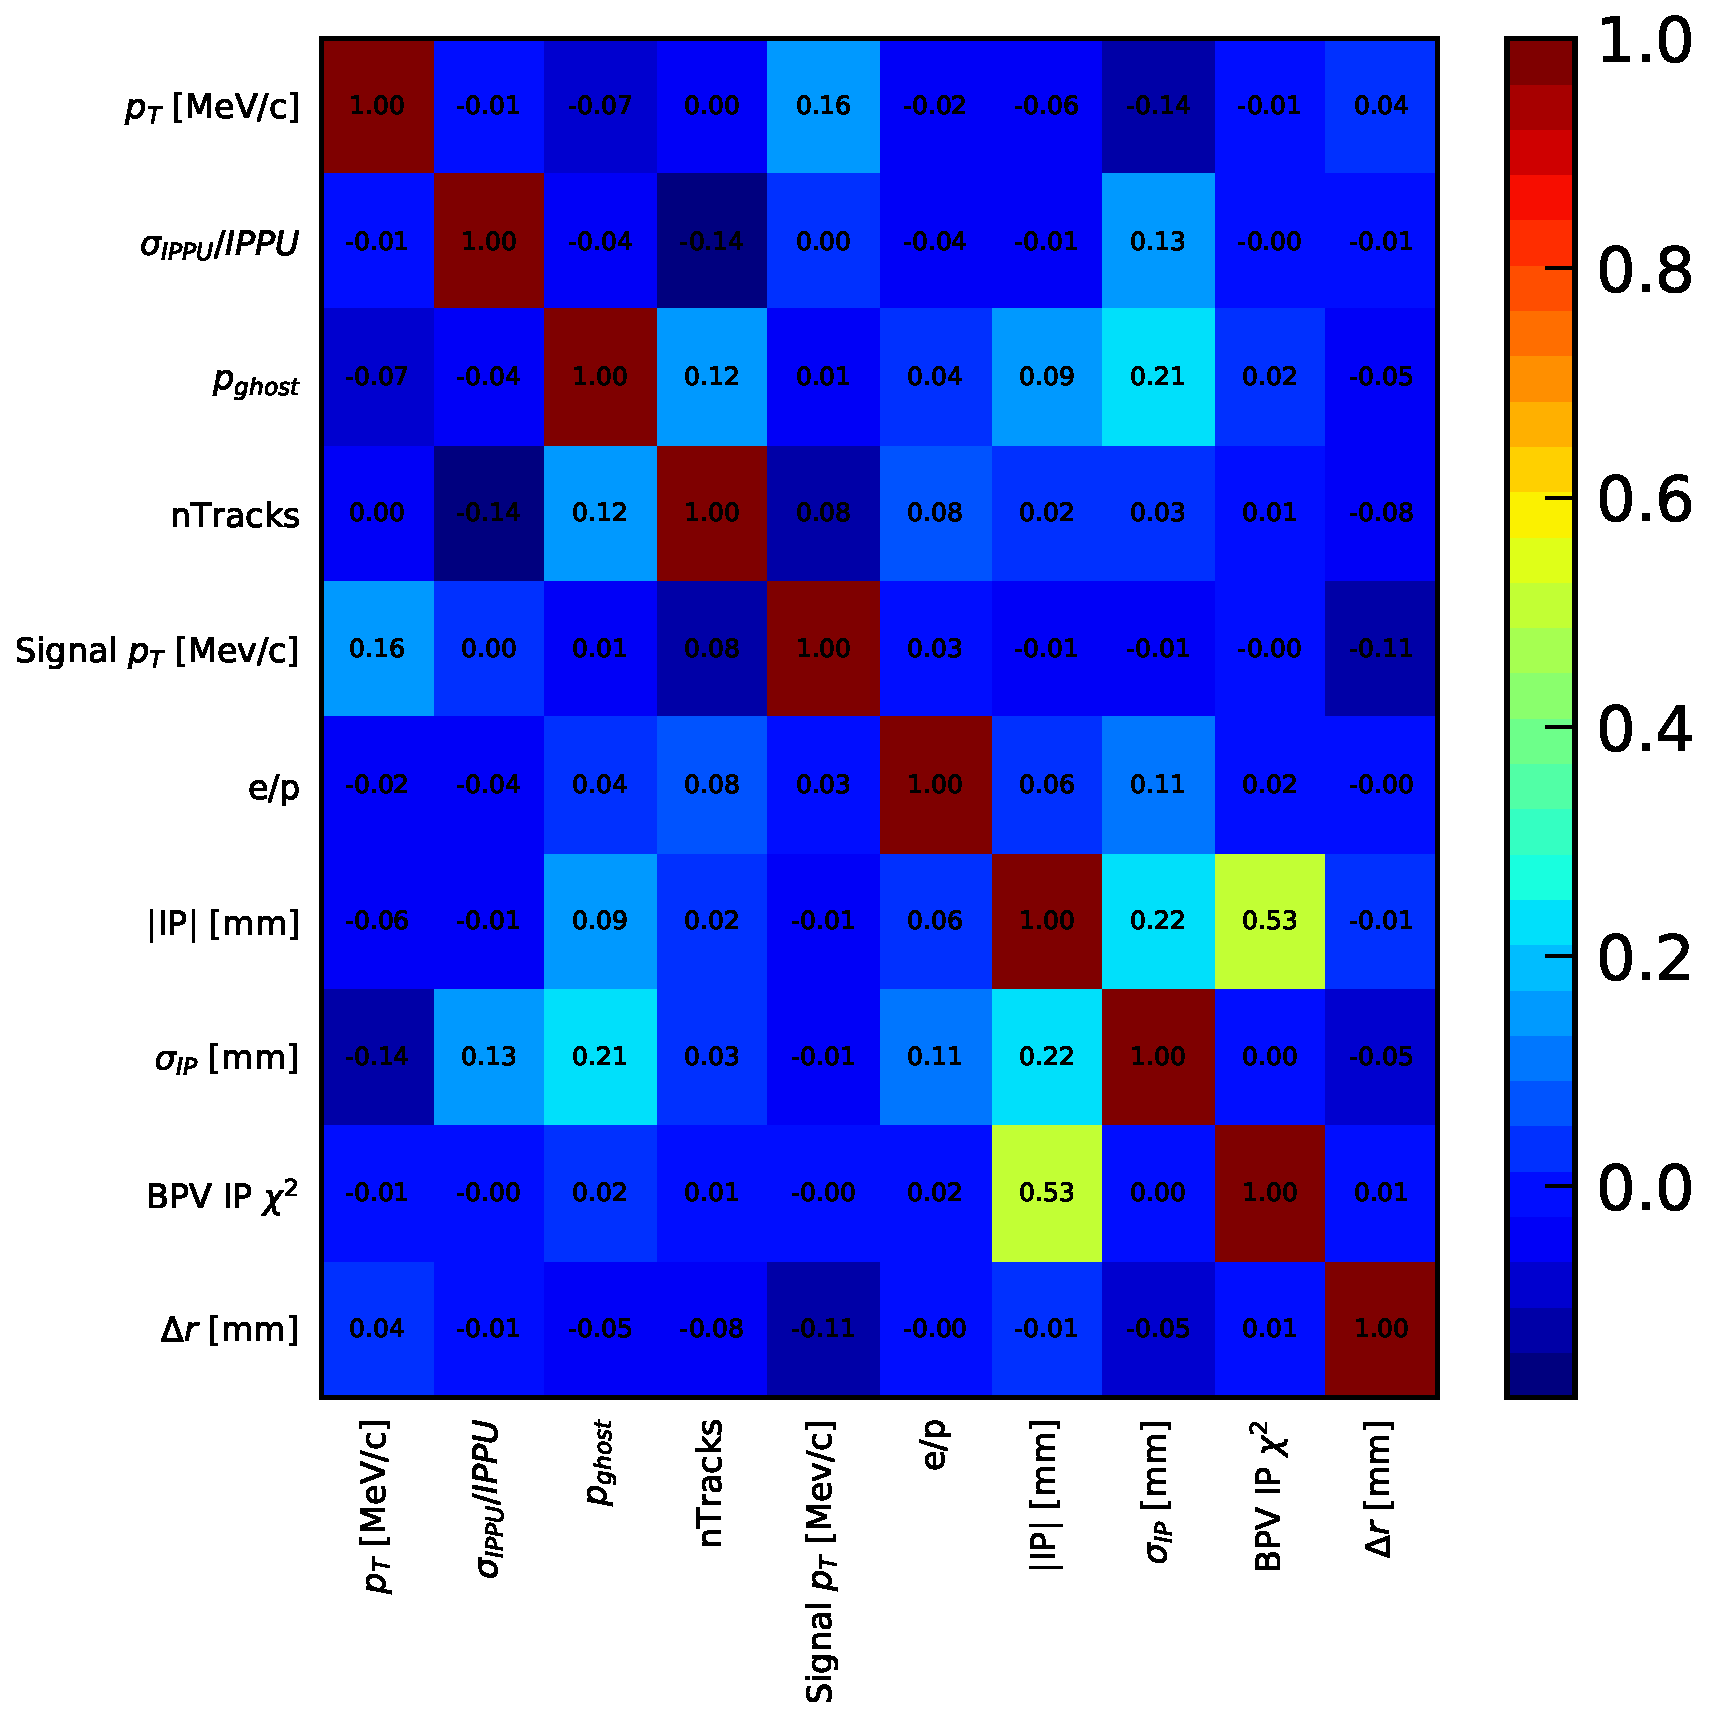
\includegraphics[width=0.47\textwidth]{04Flavourtagging/figs/OSelectronOpt/2017-12-12-vibattis-OSElectron-bdt-calibration-sWeights_Run1/FeaturesCorrRightTag_RunIcuts.pdf}
        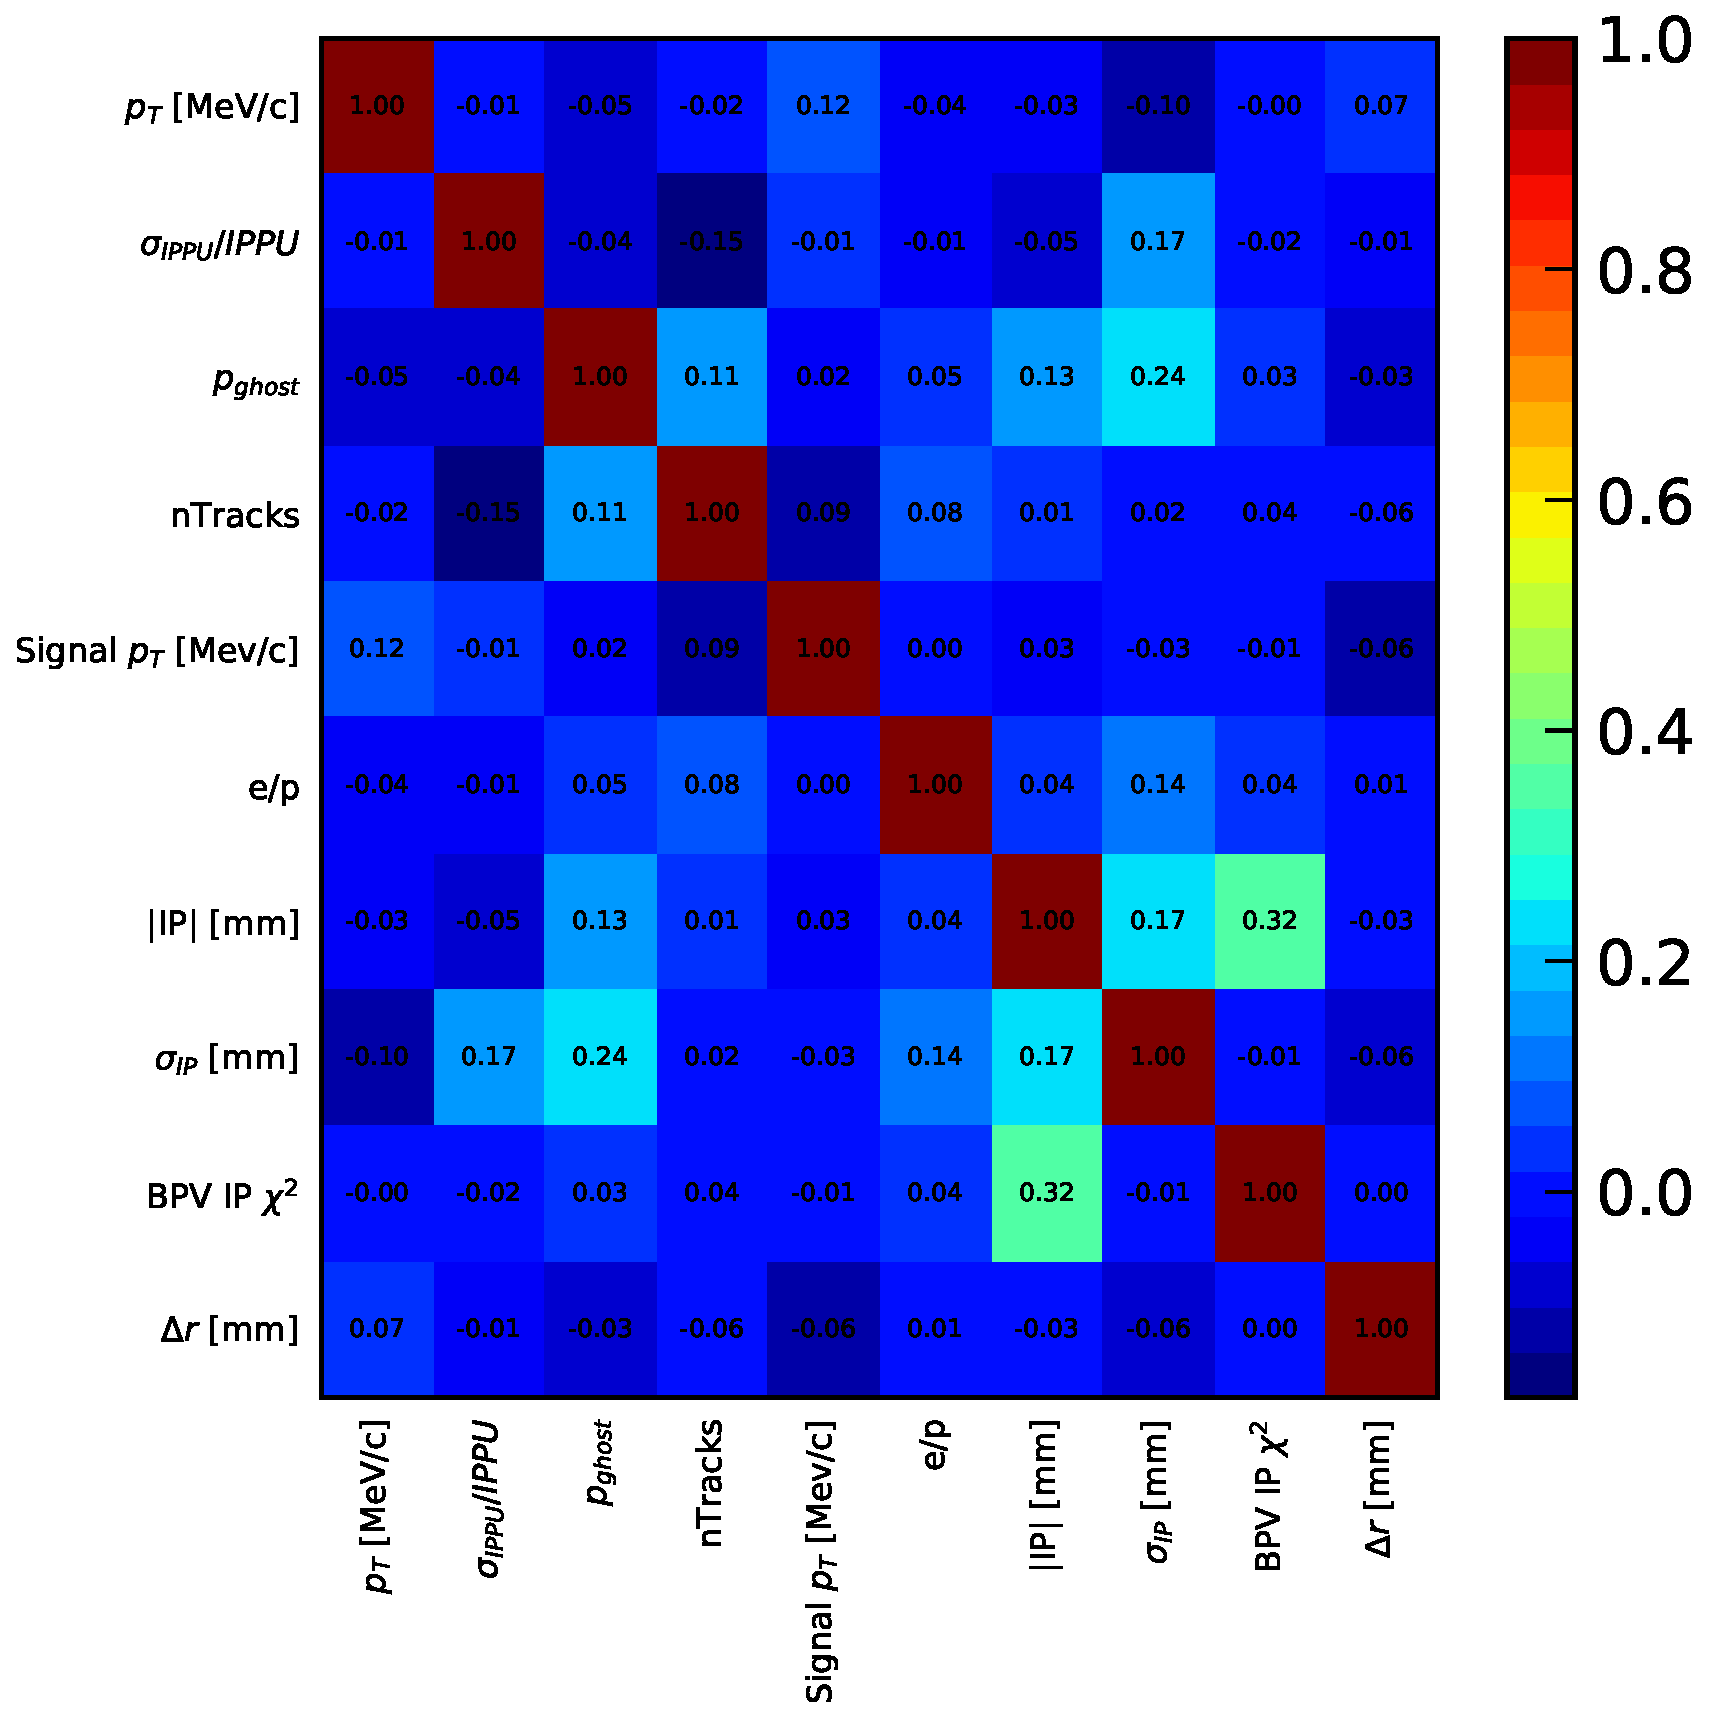
\includegraphics[width=0.47\textwidth]{04Flavourtagging/figs/OSelectronOpt/2017-12-12-vibattis-OSElectron-bdt-calibration-sWeights_Run1/FeaturesCorrWrongTag_RunIcuts.pdf} \\
        \includegraphics[width=0.47\textwidth]{04Flavourtagging/figs/OSelectronOpt/2017-12-12-vibattis-OSElectron-bdt-calibration-sWeights_Run2/FeaturesCorrRightTag_RunIIcuts.pdf}
        \includegraphics[width=0.47\textwidth]{04Flavourtagging/figs/OSelectronOpt/2017-12-12-vibattis-OSElectron-bdt-calibration-sWeights_Run2/FeaturesCorrWrongTag_RunIIcuts.pdf} \\
        \includegraphics[width=0.47\textwidth]{04Flavourtagging/figs/OSelectronOpt/2018-04-07-vibattis-OSElectron-bdt-calibration-sWeights_Run2_Bu2D0pi/FeaturesCorrRightTag_RunIIcuts.pdf}
        \includegraphics[width=0.47\textwidth]{04Flavourtagging/figs/OSelectronOpt/2018-04-07-vibattis-OSElectron-bdt-calibration-sWeights_Run2_Bu2D0pi/FeaturesCorrWrongTag_RunIIcuts.pdf} \\
        \end{center}
        \vspace{-2mm}
        \caption{Pearson correlation coefficients between the input features of the Run 1 new (top), Run 2 B2CC (middle) and Run 2 B2OC (bottom) BDT classifiers, for candidates with a correct (left) and wrong (right) decision from the \OSe~tagger.}
         \label{fig:OSecorrelations}
\end{figure}

The BDT classifier consists of an ensemble of 300 gradient-boosted decision trees~\cite{xgboost}, where each tree can have a maximum depth of 3. The objective of the classifier is a binary logistic loss function plus a quadratic regularisation term to control model complexity (with regularisation parameter $\lambda=1$). Some hyperparameters were tested by means of a cross-validation+bootstrapping method on the training set, as described in Appendix~\ref{app:oselectronappendix}. The importance (or F score) of each feature, defined as the total number of times a feature is chosen as split node by any tree in the BDT ensemble, is presented in Fig.~\ref{fig:OSeimportance}, while the \emph{partial dependence} of the predicted mistag $\eta$ (on the training set) as a function of each input feature is shown in Appendix~\ref{app:oselectronappendix}. 
The receiver operating characteristic (ROC) curves, which report the \emph{true positive rate}  
as a function of the \emph{false positive rate}, 
are shown in Fig.~\ref{fig:OSerocs}. 
The true (false) positive rate is the fraction of true, correctly (incorrectly) tagged candidates over all candidates classified as correctly tagged. 
The feature selection, BDT training and feature importance evaluation chain is repeated iteratively in order to exclude highly-correlated and poorly-important features, until the BDT performance starts to degrade significantly.

\begin{figure}[t]
        \begin{center}
        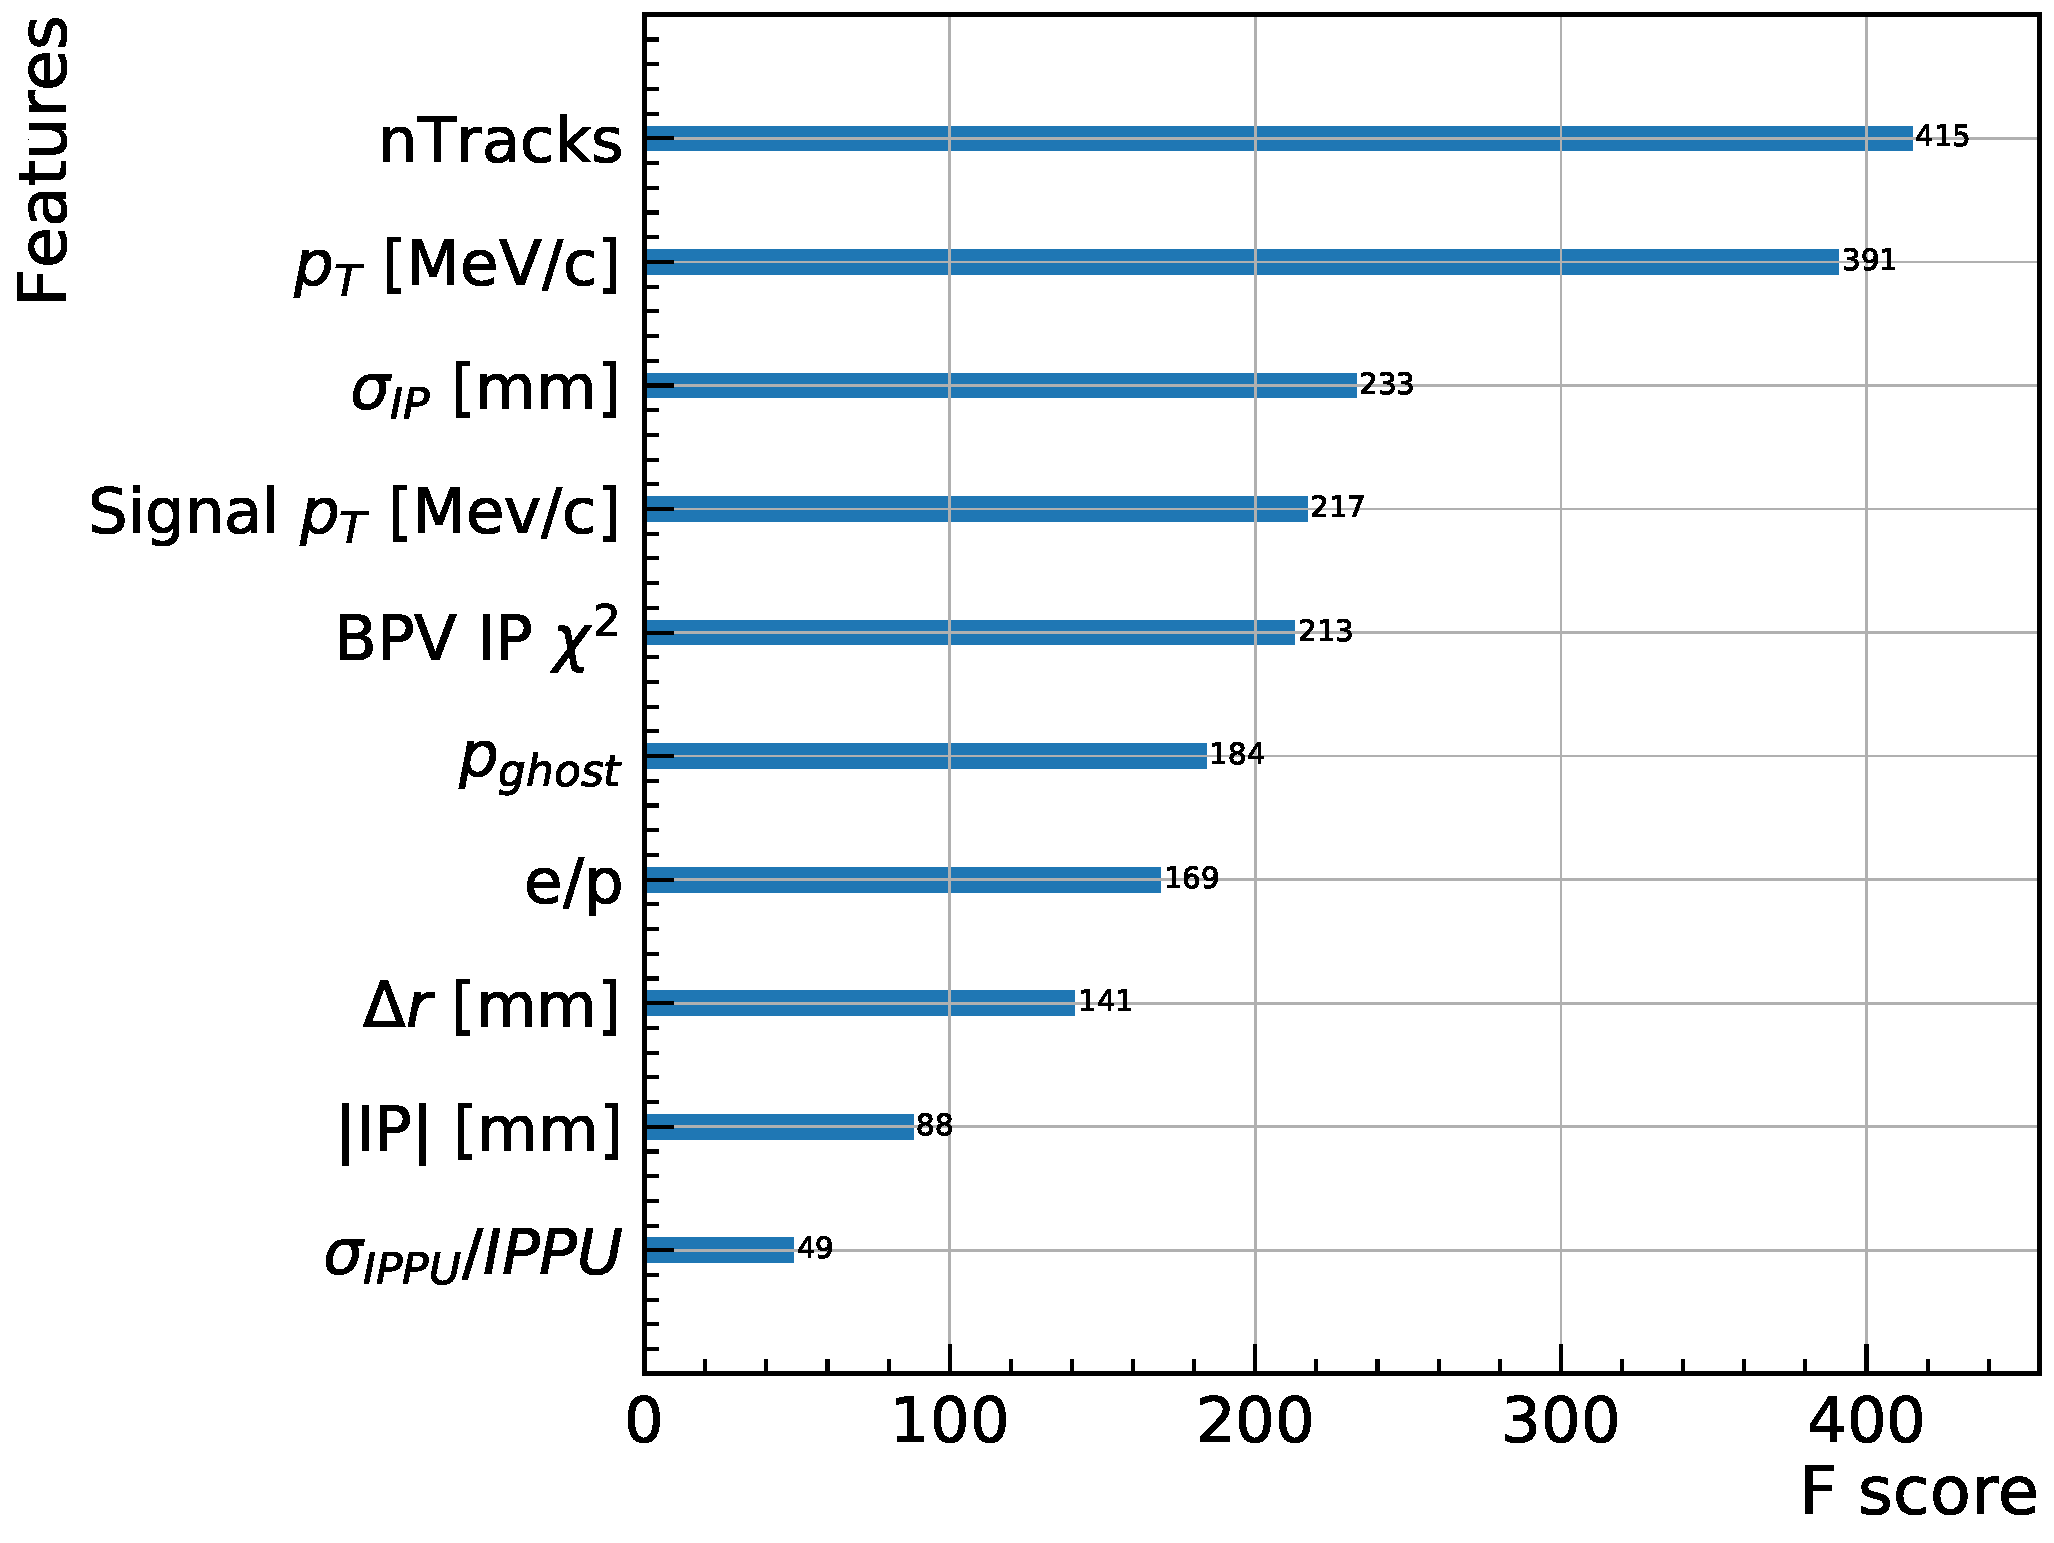
\includegraphics[width=0.4\textwidth]{04Flavourtagging/figs/OSelectronOpt/2017-12-12-vibattis-OSElectron-bdt-calibration-sWeights_Run1/Importance_RunIcuts.pdf}
        \includegraphics[width=0.4\textwidth]{04Flavourtagging/figs/OSelectronOpt/2017-12-12-vibattis-OSElectron-bdt-calibration-sWeights_Run2/Importance_RunIIcuts.pdf} \\
        \includegraphics[width=0.4\textwidth]{04Flavourtagging/figs/OSelectronOpt/2018-04-07-vibattis-OSElectron-bdt-calibration-sWeights_Run2_Bu2D0pi/Importance_RunIIcuts.pdf}
        \end{center}
        \vspace{-2mm}
        \caption{Feature importance for the BDT classifiers of the Run 1 new (top left), Run 2 B2CC (top right) and Run 2 B2OC (bottom) implementations of the \OSe~tagger.}
         \label{fig:OSeimportance}
\end{figure}

\begin{figure}[t]
        \begin{center}
        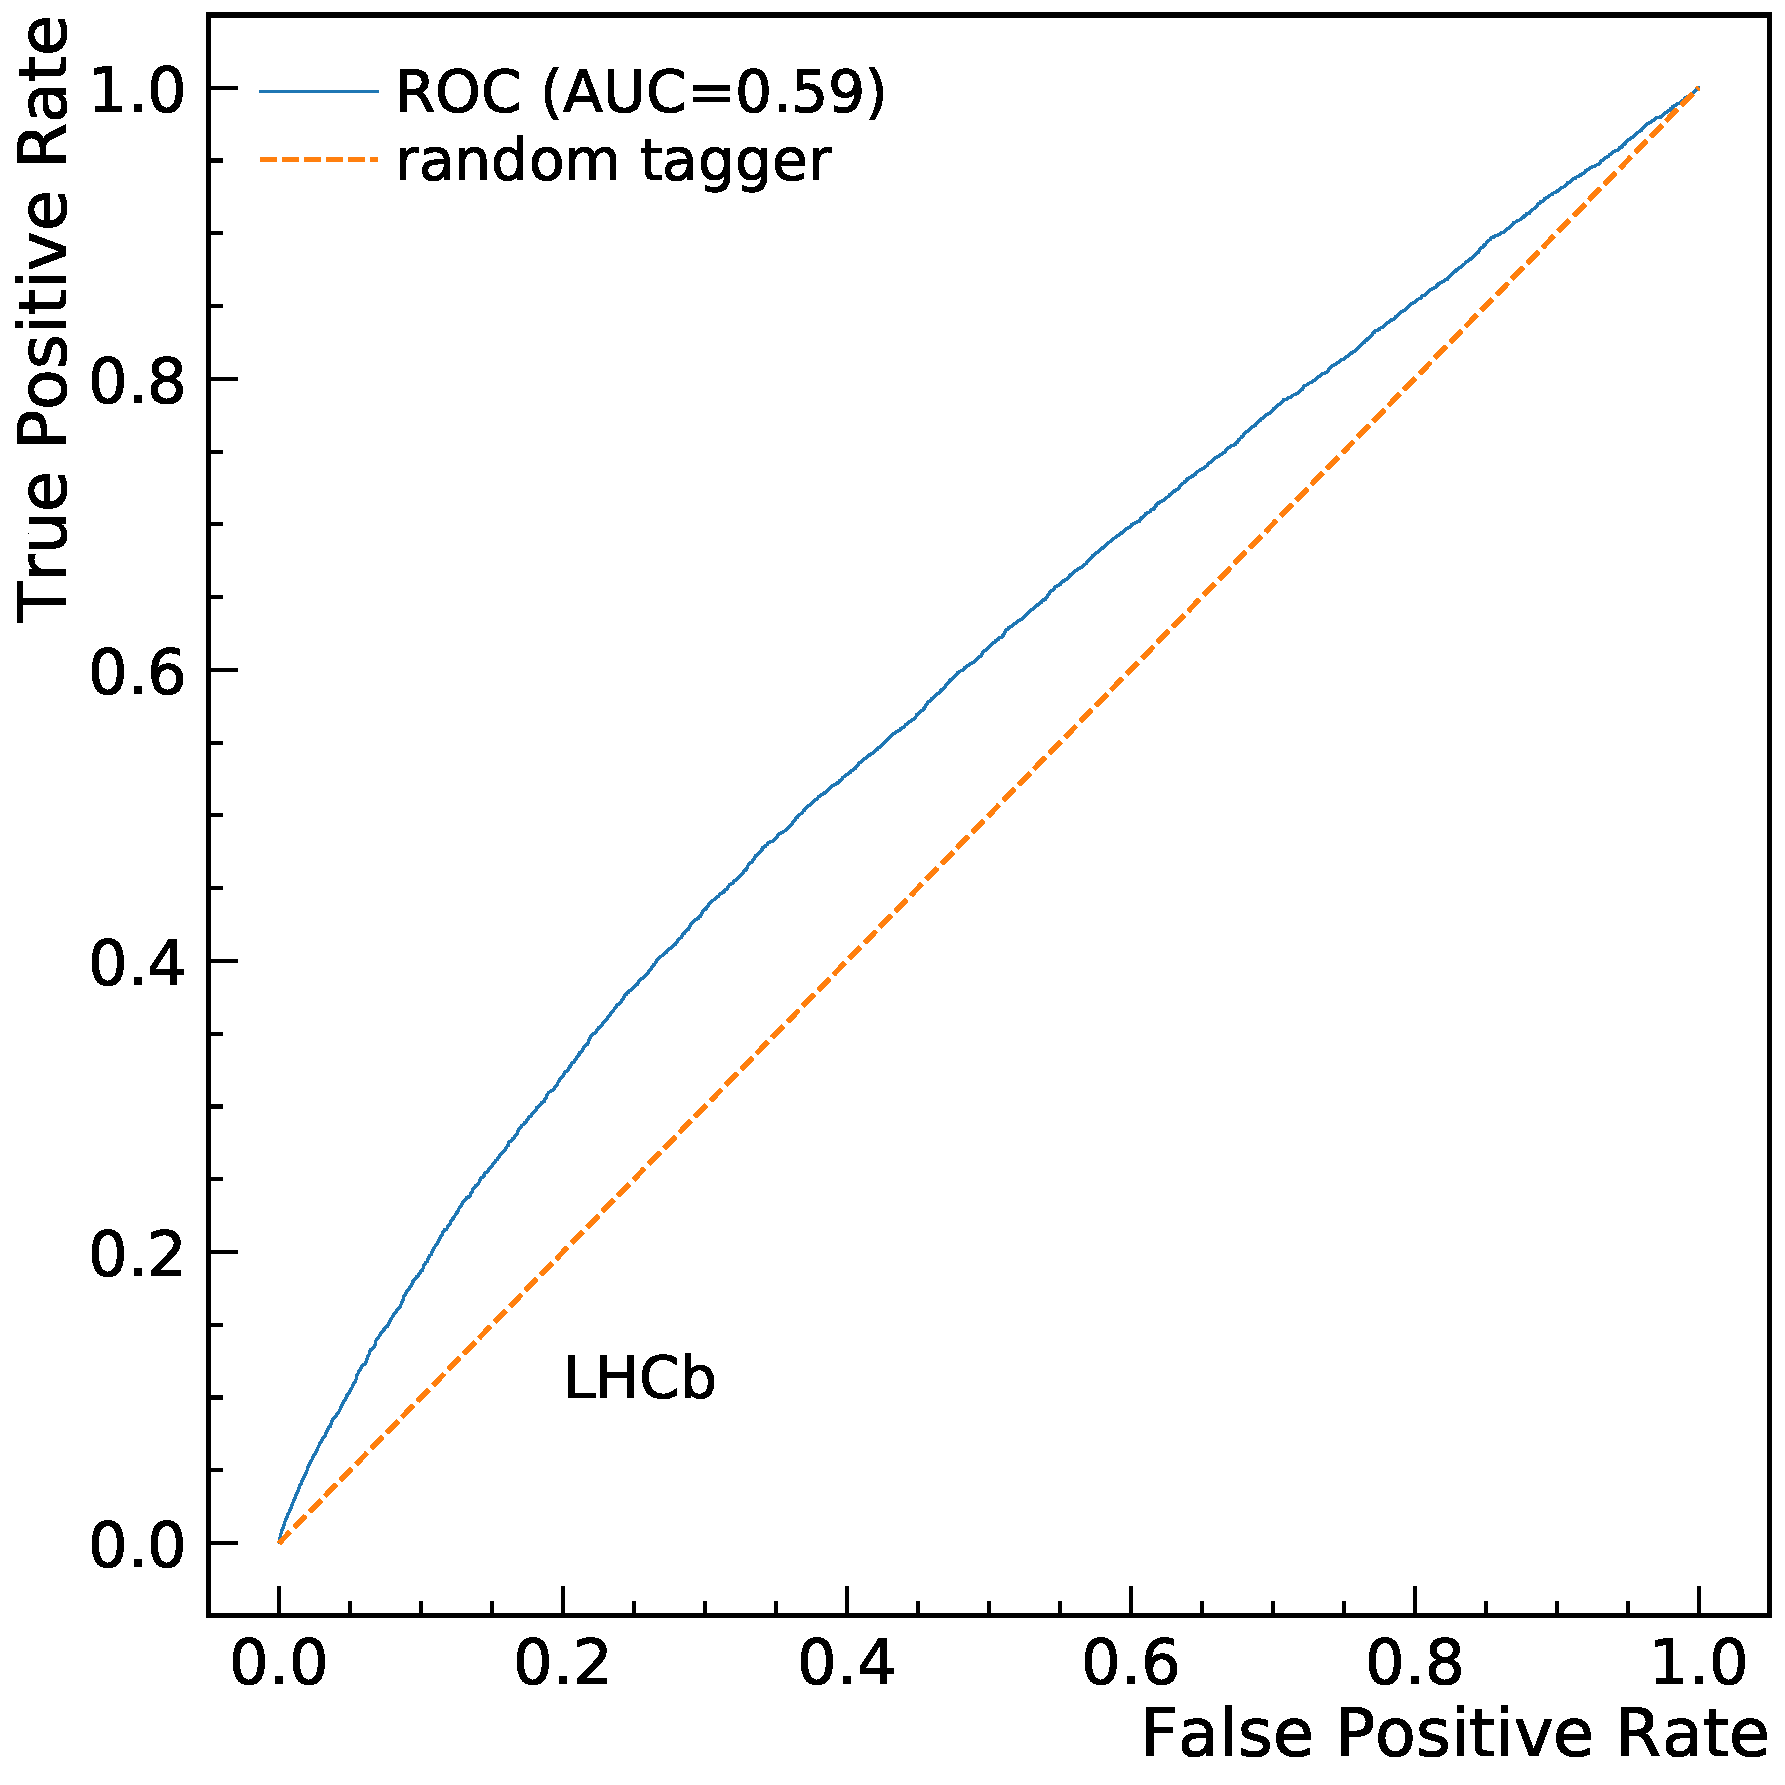
\includegraphics[width=0.4\textwidth]{04Flavourtagging/figs/OSelectronOpt/2017-12-12-vibattis-OSElectron-bdt-calibration-sWeights_Run1/ROC_RunIcuts.pdf}
        \includegraphics[width=0.4\textwidth]{04Flavourtagging/figs/OSelectronOpt/2017-12-12-vibattis-OSElectron-bdt-calibration-sWeights_Run2/ROC_RunIIcuts.pdf} \\
        \includegraphics[width=0.4\textwidth]{04Flavourtagging/figs/OSelectronOpt/2018-04-07-vibattis-OSElectron-bdt-calibration-sWeights_Run2_Bu2D0pi/ROC_RunIIcuts.pdf}
        \end{center}
        \vspace{-2mm}
        \caption{True positive rate as a function of the false positive rate (ROC curves) for the BDT classifiers of the Run 1 new (top left), Run 2 B2CC (top right) and Run 2 B2OC (bottom) implementations of \OSe. The obtained ROC curves are represented in blue, while the expected ROC curve in case of random tag decision is shown as a dashed orange line. For each BDT, the \emph{Area Under the} ROC \emph{Curve} (AUC score) is reported as well.}
         \label{fig:OSerocs}
\end{figure}

For each candidate, the BDT predicts the probability $P$ that such candidates is correctly tagged. In order to obtain a mistag probability $\eta$, the following transformation is applied on both $P$ and tagging decision $d$:
\begin{equation}
        (\eta, d) \rightarrow \begin{cases} (P, -d) &\text{if $P\leq0.5$} \\ (1-P, d) &\text{otherwise} \end{cases}        
\end{equation} 
The distributions of $\eta$ for training and test samples, splitted per target value, are shown in Fig.~\ref{fig:OSeetapredict}.

\begin{figure}[t]
        \begin{center}
        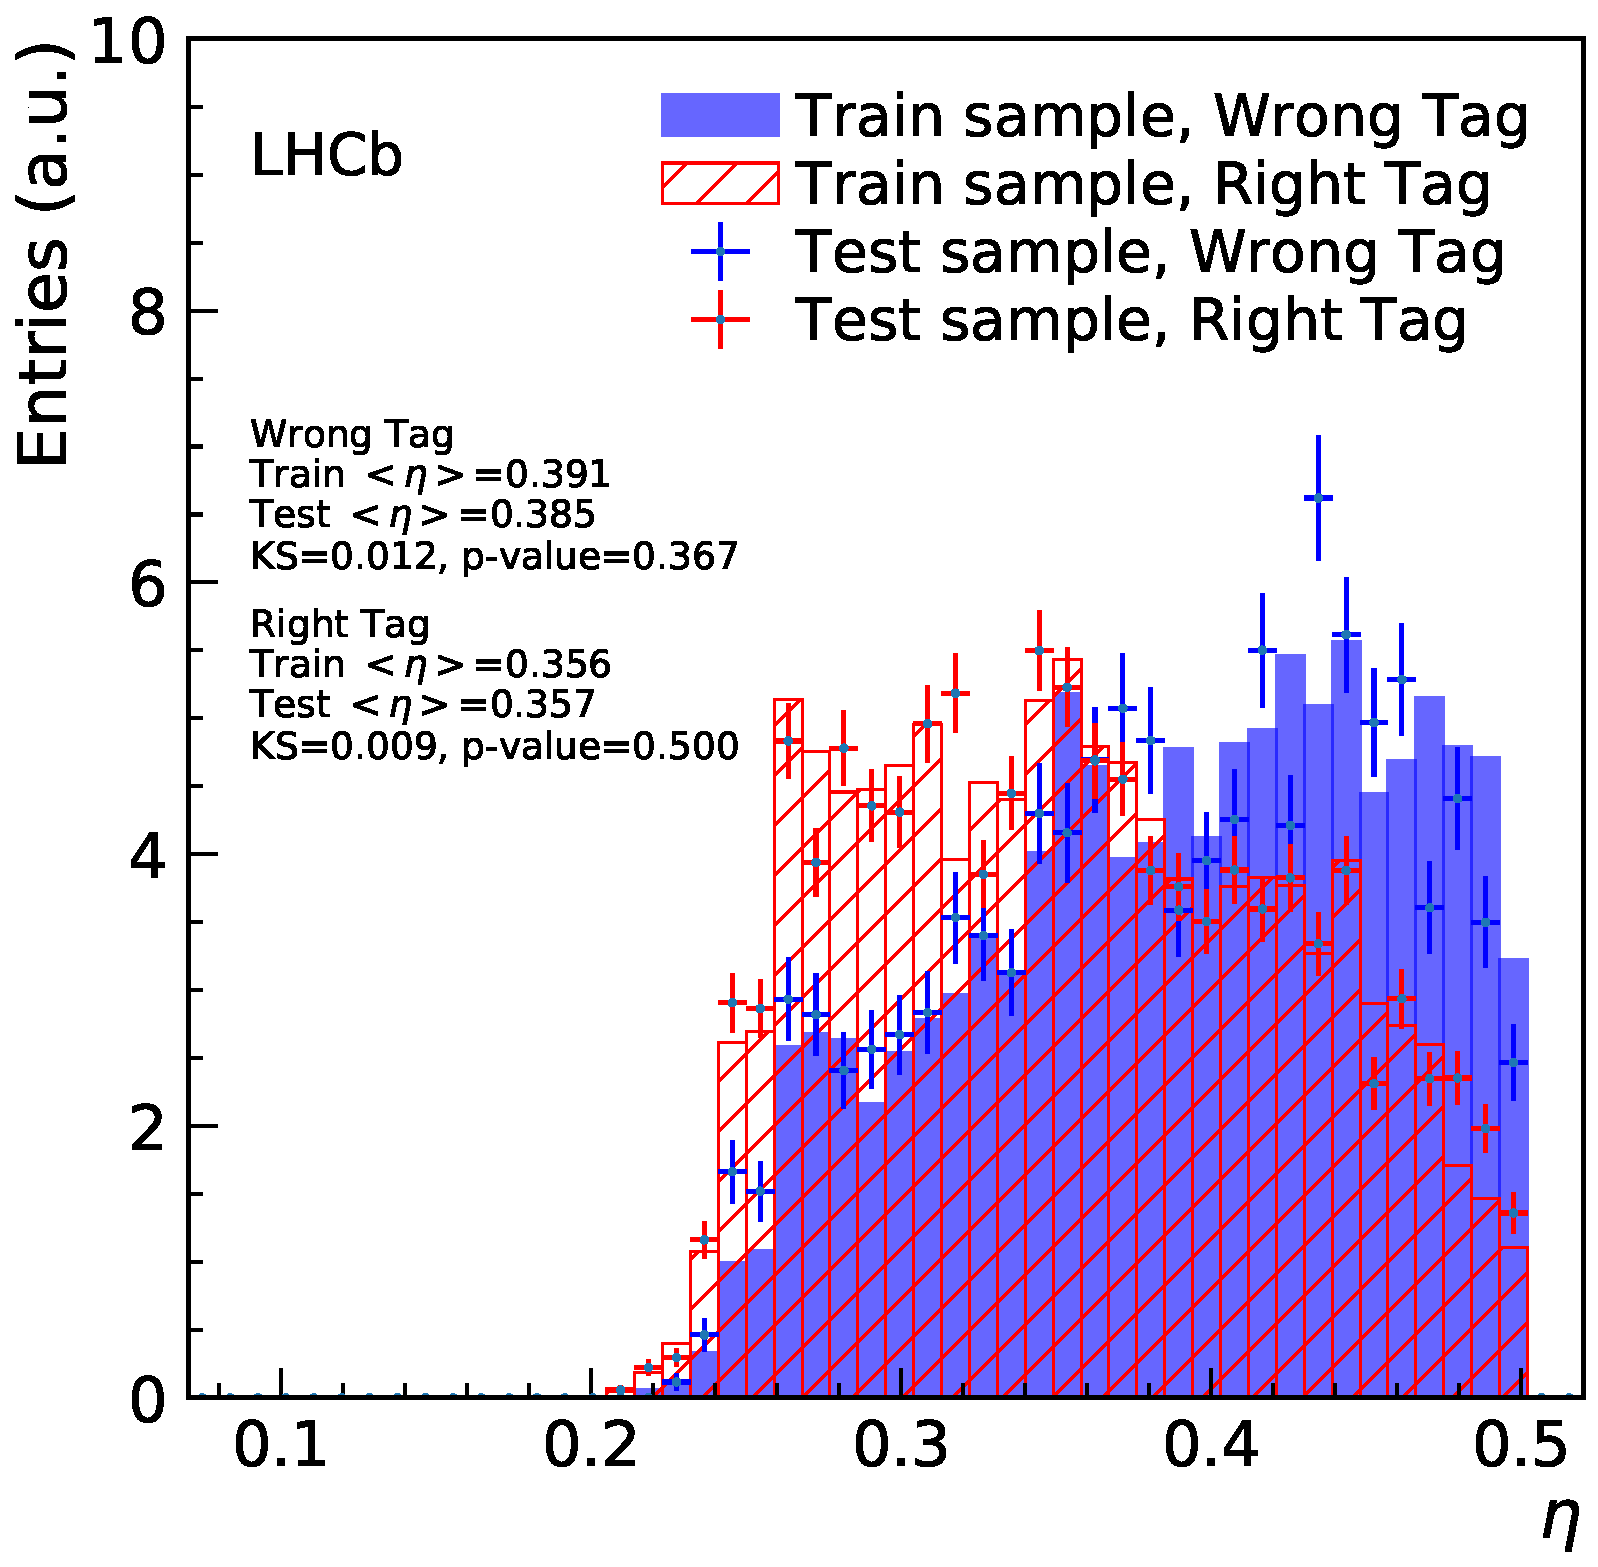
\includegraphics[width=0.4\textwidth]{04Flavourtagging/figs/OSelectronOpt/2017-12-12-vibattis-OSElectron-bdt-calibration-sWeights_Run1/PredictedEta_RunIcuts.pdf}
        \includegraphics[width=0.4\textwidth]{04Flavourtagging/figs/OSelectronOpt/2017-12-12-vibattis-OSElectron-bdt-calibration-sWeights_Run2/PredictedEta_RunIIcuts.pdf}
        \includegraphics[width=0.4\textwidth]{04Flavourtagging/figs/OSelectronOpt/2018-04-07-vibattis-OSElectron-bdt-calibration-sWeights_Run2_Bu2D0pi/PredictedEta_RunIIcuts.pdf}
        \end{center}
        \vspace{-2mm}
        \caption{\emph{sWeighted} distributions of the mistag probability $\eta$ predicted by the BDT classifiers of the Run 1 new (top left), Run 2 B2CC (top right) and Run 2 B2OC (bottom) versions of the \OSe~tagger. 
          The blue-solid (red-hatched) histogram represents the training data for candidates having the wrong (right) tag decision. 
          The blue (red) points indicate the test data for candidates with wrong (right) tag decision. 
          The overtraining is checked, separately for candidates with wrong and right tag decision,
          by means of a Kologorov-Smirnov (KS) test to measure the compatibility between training data and test data.
          The conventional value of $0.05$ is chosen as significance level to reject the hypothesis of compatibility.}
        \label{fig:OSeetapredict}
\end{figure}

%%%%%%%%%%%%%%%%%%%%%%%%%%%%%%%%%%%%%%%%%%%%%%%%%%%%

\subsection{Performance evaluation}

%%%%%%%%%%%%%%%%%%%%%%%%%%%%%%%%%%%%%%%%%%%%%%%%%%%%

\subsubsection[Performance on $B^+\to J/\psi K^+$ and $B^+\to \Dzb \pi^+$ data]{Performance on \boldmath{$B^+\to J/\psi K^+$} and \boldmath{$B^+\to \Dzb \pi^+$} data}
\label{sec:tagging:OSePerf1}

Once the BDT is trained on the training ssample, the mistag $\eta$ is predicted for each candidate using the evaluation samples. Then, a two-fold evaluation is applied:
\begin{itemize}[noitemsep,topsep=0pt]
        \item the mistag calibration is determined on the first evaluation sample. The obtained calibration is then applied to the second evaluation sample, and a calibrated per-event tagging power is computed on the latter;
        \item same as above, but with the two evaluation samples swapped.
\end{itemize}
The calibrated per-event tagging power is computed by considering, for each tagged $B$ candidate, only the tagging particle with the highest transverse momentum.
The calibration model consists of a first order natural spline with a logistic link function.
The result of these calibrations are shown in Fig.~\ref{fig:OSeetacalib}.
The calibrated per-event tagging power is reported in Table~\ref{tab:OSeperformanceevalset}.

\begin{figure}[t]
        \begin{center}
        \includegraphics[width=0.4\textwidth]{04Flavourtagging/figs/OSelectronOpt/RunIEval_Bu2JpsiKst/eval_on_I.pdf}
        \includegraphics[width=0.4\textwidth]{04Flavourtagging/figs/OSelectronOpt/RunIEval_Bu2JpsiKst/eval_on_II.pdf} \\
        \includegraphics[width=0.4\textwidth]{04Flavourtagging/figs/OSelectronOpt/RunIIEval_Bu2JpsiKst/eval_on_I.pdf}
        \includegraphics[width=0.4\textwidth]{04Flavourtagging/figs/OSelectronOpt/RunIIEval_Bu2JpsiKst/eval_on_II.pdf} \\
        \includegraphics[width=0.4\textwidth]{04Flavourtagging/figs/OSelectronOpt/RunIIEval_Bu2D0Pi/eval_on_I.pdf}
        \includegraphics[width=0.4\textwidth]{04Flavourtagging/figs/OSelectronOpt/RunIIEval_Bu2D0Pi/eval_on_II.pdf}
        \end{center}
        \vspace{-2mm}
        \caption{\OSe~mistag calibration results for the (top) Run 1 new, (middle) Run 2 B2CC and (bottom) Run 2 B2OC optimisations. Left: calibration obtained on the second evaluation sample plotted together with the first evaluation sample. Right: calibration obtained on the first evaluation sample plotted together with the second evaluation sample. The \emph{sWeighted} data sample is shown as black points. The green (yellow) band indicates the 68\% (95\%) C.L. interval for the fitted calibration functions.}
        \label{fig:OSeetacalib}
\end{figure}

\begin{table}[t]
	\centering
        \caption{Calibrated, per-event tagging power $\effeff$ (in $\%$) of the \OSe~algorithms obtained on the evaluation sets of each \OSe~implementation. The errors include both statistical uncertainty and uncertainties from the calibration procedure. The average is computed by assuming uncorrelated measurements.}
         \label{tab:OSeperformanceevalset}
        \begin{tabular}{llll}
        \toprule
        Algorithm & set 1 & set 2 & average  \\
        \midrule
        Run 1 new & $0.513\pm0.040$ & $0.496\pm0.038$ & $0.504\pm0.028$ \\
        Run 2 B2CC & $0.324\pm0.031$ & $0.364\pm0.033$ & $0.343\pm0.023$ \\
        Run 2 B2OC & $0.455\pm0.043$ & $0.434\pm0.041$ & $0.444\pm0.030$ \\
        \bottomrule
        \end{tabular}
\end{table}

%%%%%%%%%%%%%%%%%%%%%%%%%%%%%%%%%%%%%%%%%%%%%%%%%%%%

\subsubsection[Performance on $B^0\to D^-\pi^+$ data]{Performance on \boldmath{$B^0\to D^-\pi^+$} data}
\label{sec:tagging:OSePerf2}

The performance (tagging efficiency, mistag probability, tagging power) of the calibrated \OSe~tagger is evaluated on Run 1 (2012) and Run 2 (2016) \emph{sWeighted} data samples of $B^0\to D^-\pi^+$ decays.
These decays ensure a robust estimation of the performance thanks to the high statistics collected at LHCb. Moreover, this channel was not exploited in the development of
the \OSe~tagger, so that it constitutes an independent validation of these algorithms. The performance of the other OS taggers (\OSmu, \OSK, \OSc, \OSvtx, and their combination) is presented
as well in this section in order to provide a complete overview.

The calibration and the performance evaluation are done as follows:
\begin{itemize}[noitemsep,topsep=0pt]
  \item each sample (Run 1 and Run 2) is split randomly in two subsamples;
    \item the calibrations are found on one subsample for all OS taggers;
      \item the obtained calibrations are applied to the other subsample, and the calibrated performance is evaluated.
        \item the calibrated OS taggers are combined, the combination is calibrated in order to correct for effects due to correlations among taggers, and the performance of the calibrated combination is evaluated.
\end{itemize}

The calibrations are obtained via a time-dependent analysis of the $B^0\to D^-\pi^+$ decays, where acceptance and resolution effects are neglected as described in Ref.~\cite{EPM}; moreover, the Cabibbo-suppressed decay mode $B^0\to D^+\pi^-$ is ignored as well.
The chosen model 
$\omega(\eta)$ for each tagger is a GLM model with a logistic link function, and a first order spline as basis function. The results of the calibration and the mistag distribution of each \OSe~implementation are shown in Figs.~\ref{fig:OSePerfCalib1} and~\ref{fig:OSePerfCalib3}; the calibration and the mistag of the corresponding OS combinations are also reported in Figs.~\ref{fig:OSePerfCalib2} and~\ref{fig:OSePerfCalib4}.
 
\begin{figure}[ht!]
        \centering
        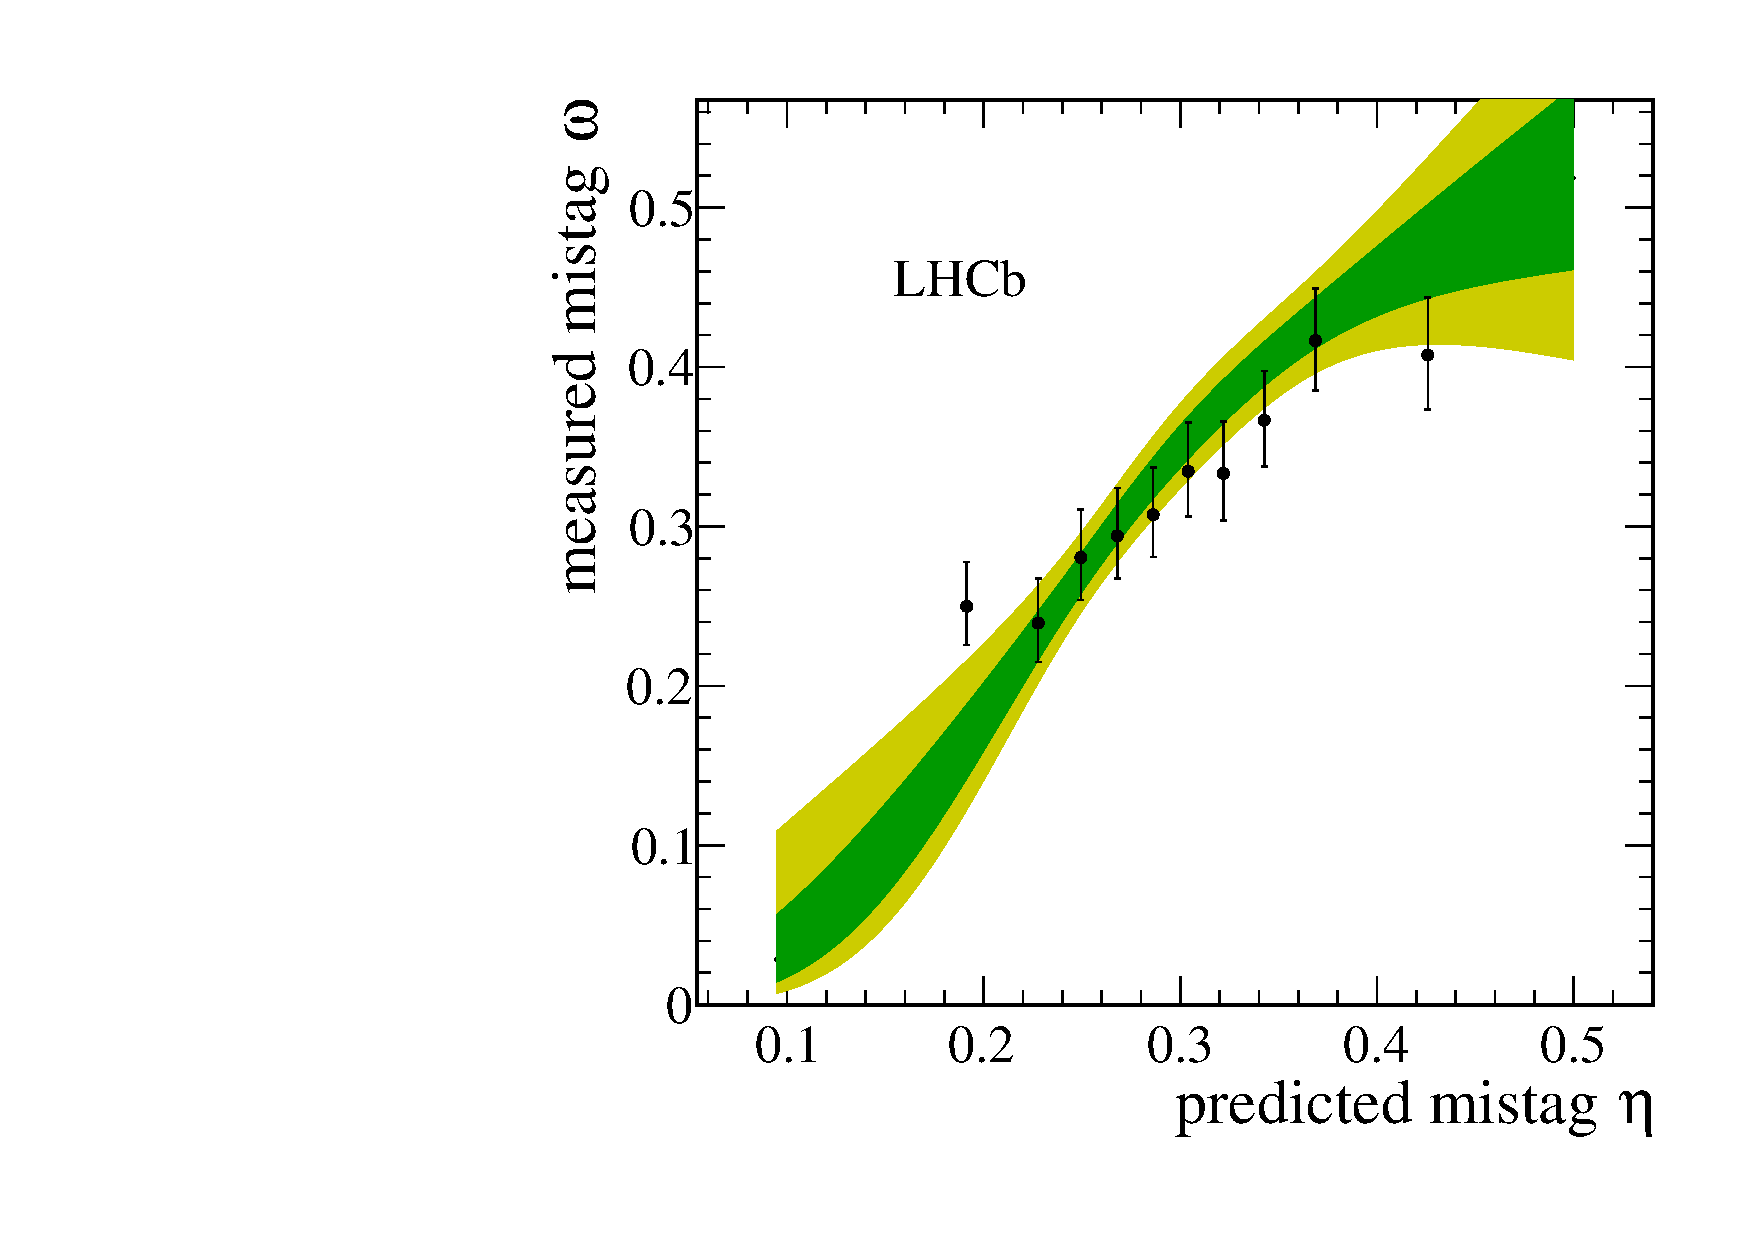
\includegraphics[width=0.26\textwidth]{04FlavourTagging/figs/OSelectronOpt/run1data_old/OS_Electron_InputCalibration.pdf}
        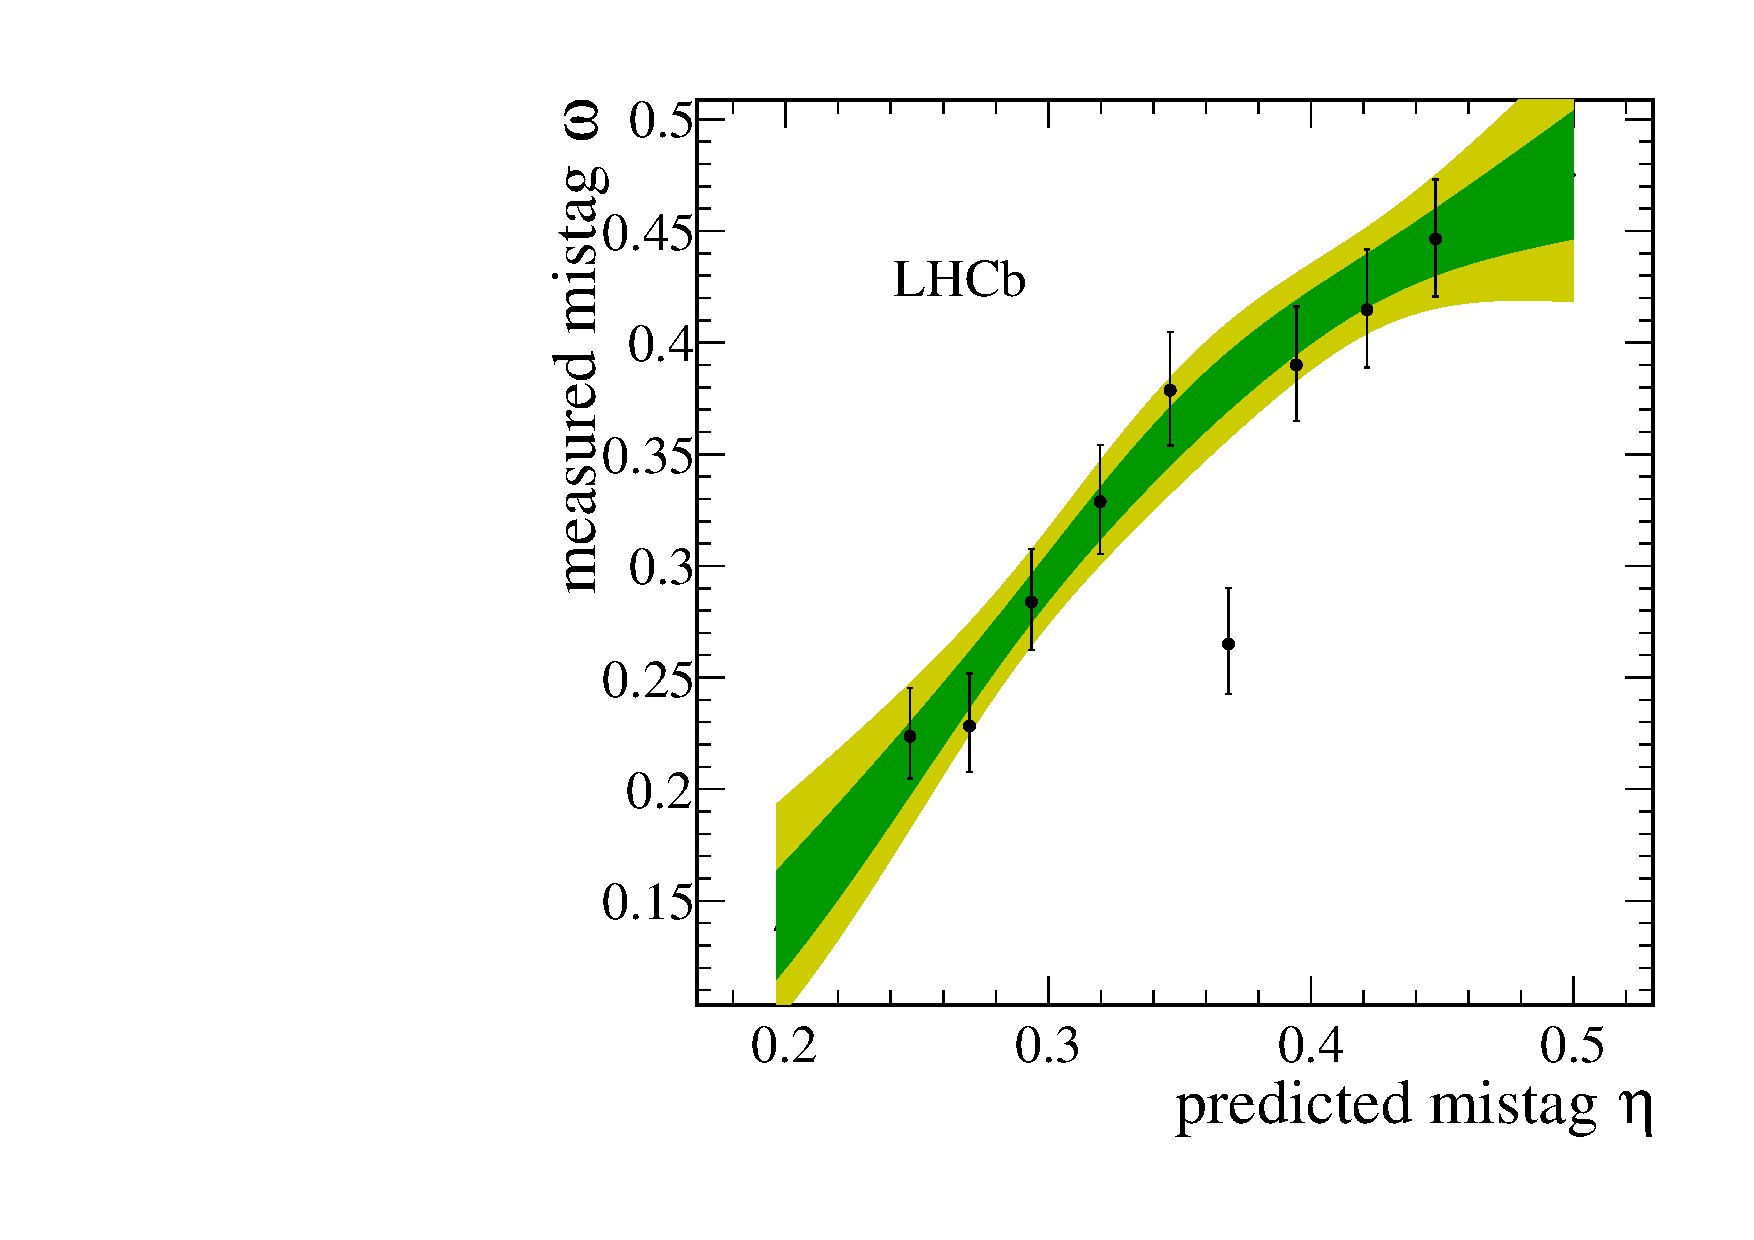
\includegraphics[width=0.26\textwidth]{04FlavourTagging/figs/OSelectronOpt/run1data_new/OS_Electron_InputCalibration.pdf} \\
        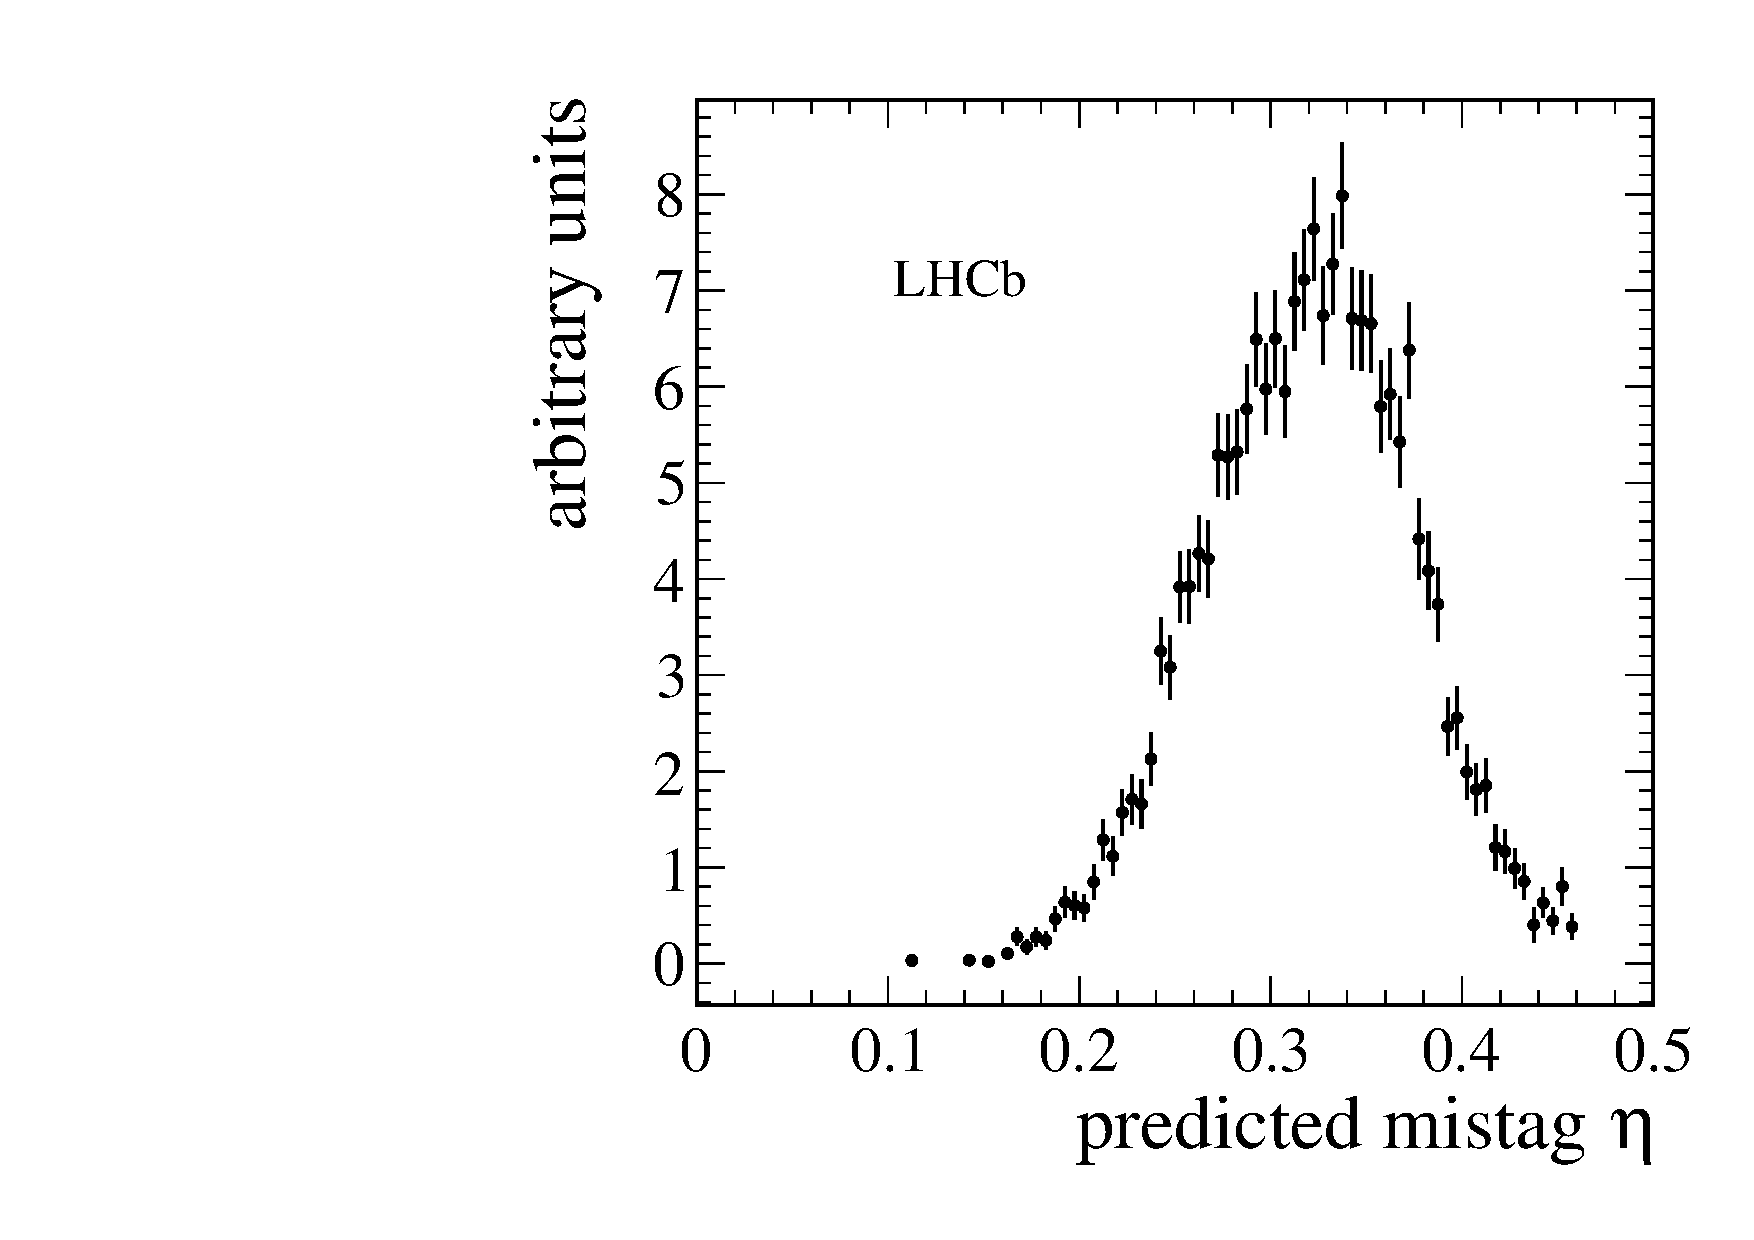
\includegraphics[width=0.26\textwidth]{04FlavourTagging/figs/OSelectronOpt/run1data_old/OS_Electron_EtaDist.pdf}
        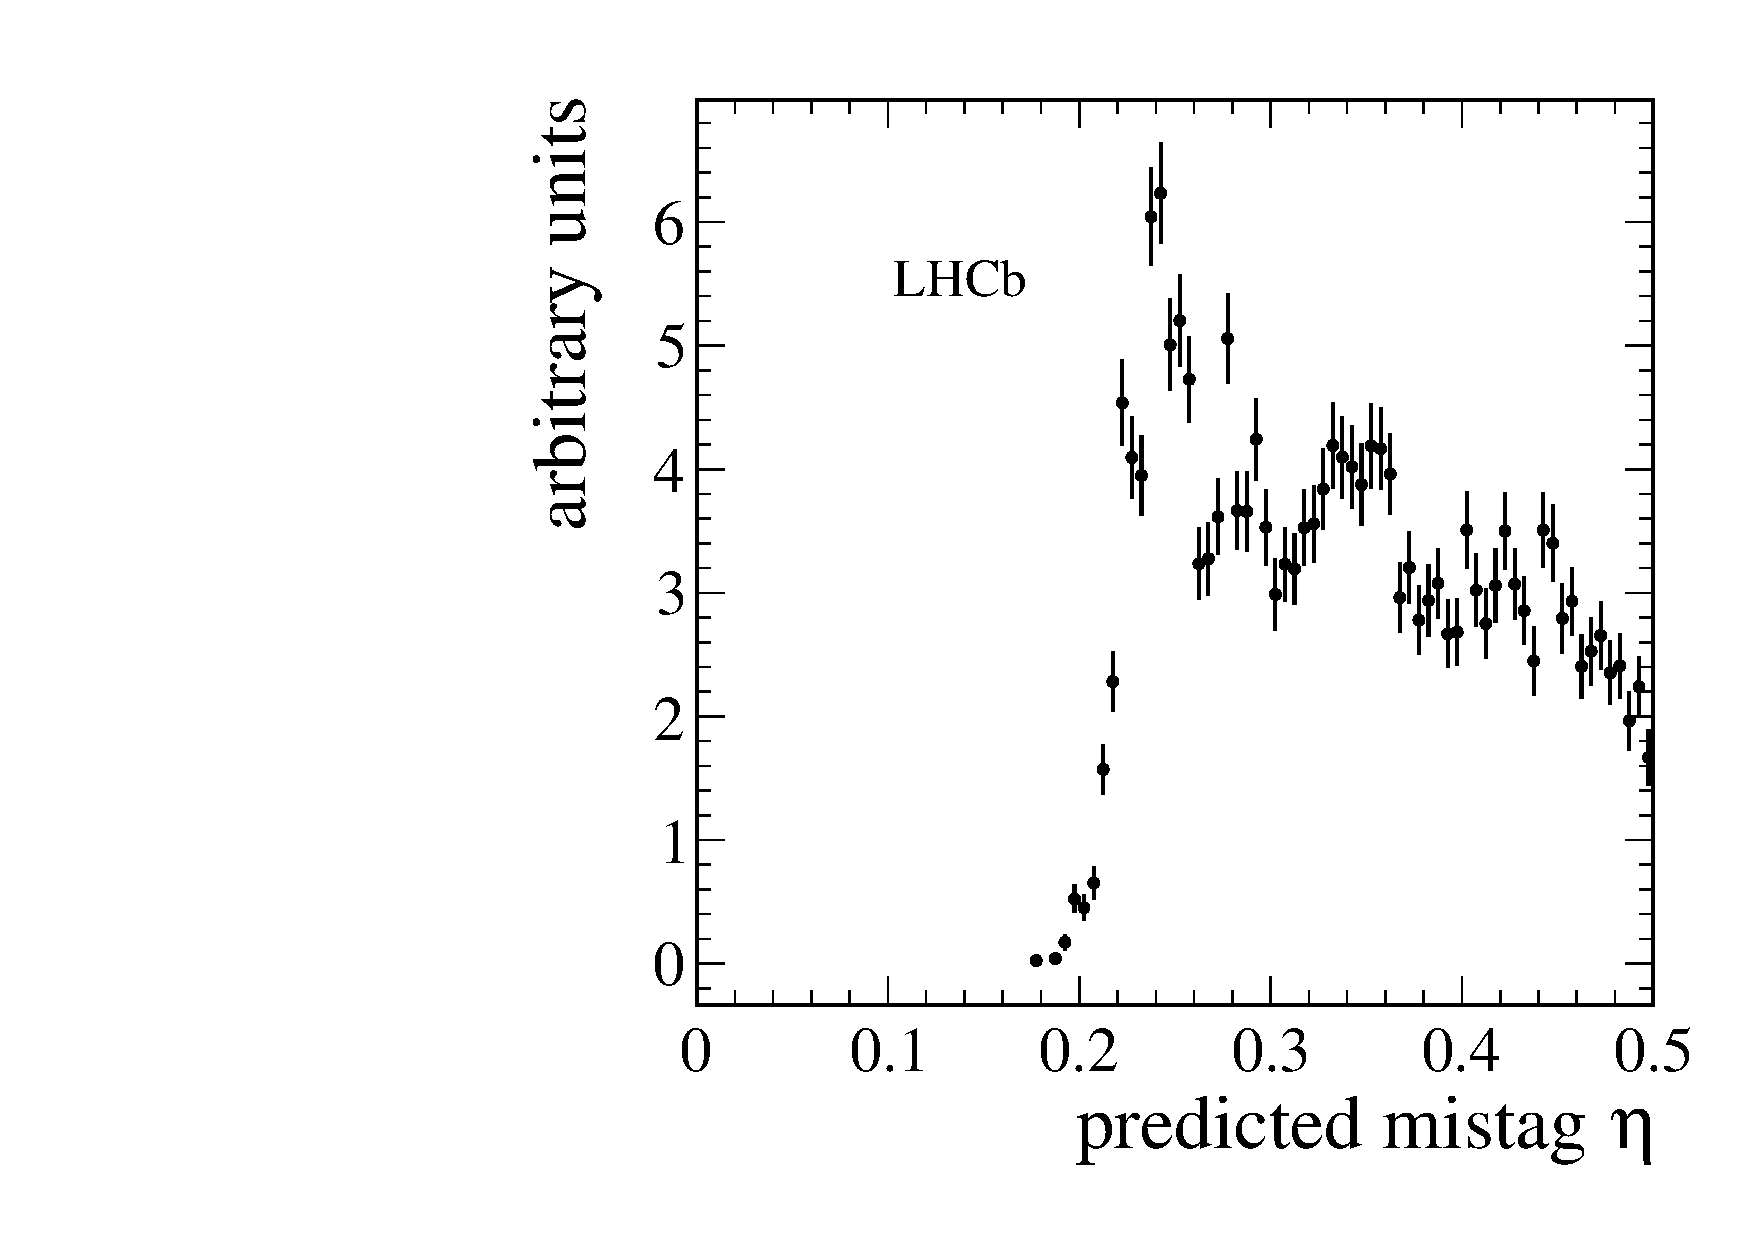
\includegraphics[width=0.26\textwidth]{04FlavourTagging/figs/OSelectronOpt/run1data_new/OS_Electron_EtaDist.pdf}
        \vspace{-2mm}
        \caption{Top: mistag calibration results on \emph{sWeighted} Run 1 $B^0\to D^-\pi^+$ data for the Run 1 old (left) and Run 1 new (right) versions of the \OSe~tagger. The \emph{sWeighted} data sample is shown as black points. The green (yellow) band indicates the 68\% (95\%) C.L. interval for the fitted calibration functions. Bottom: distributions of the uncalibrated mistag $\eta$.}
        \label{fig:OSePerfCalib1}
\end{figure}

\begin{figure}[hb!]
  \centering
  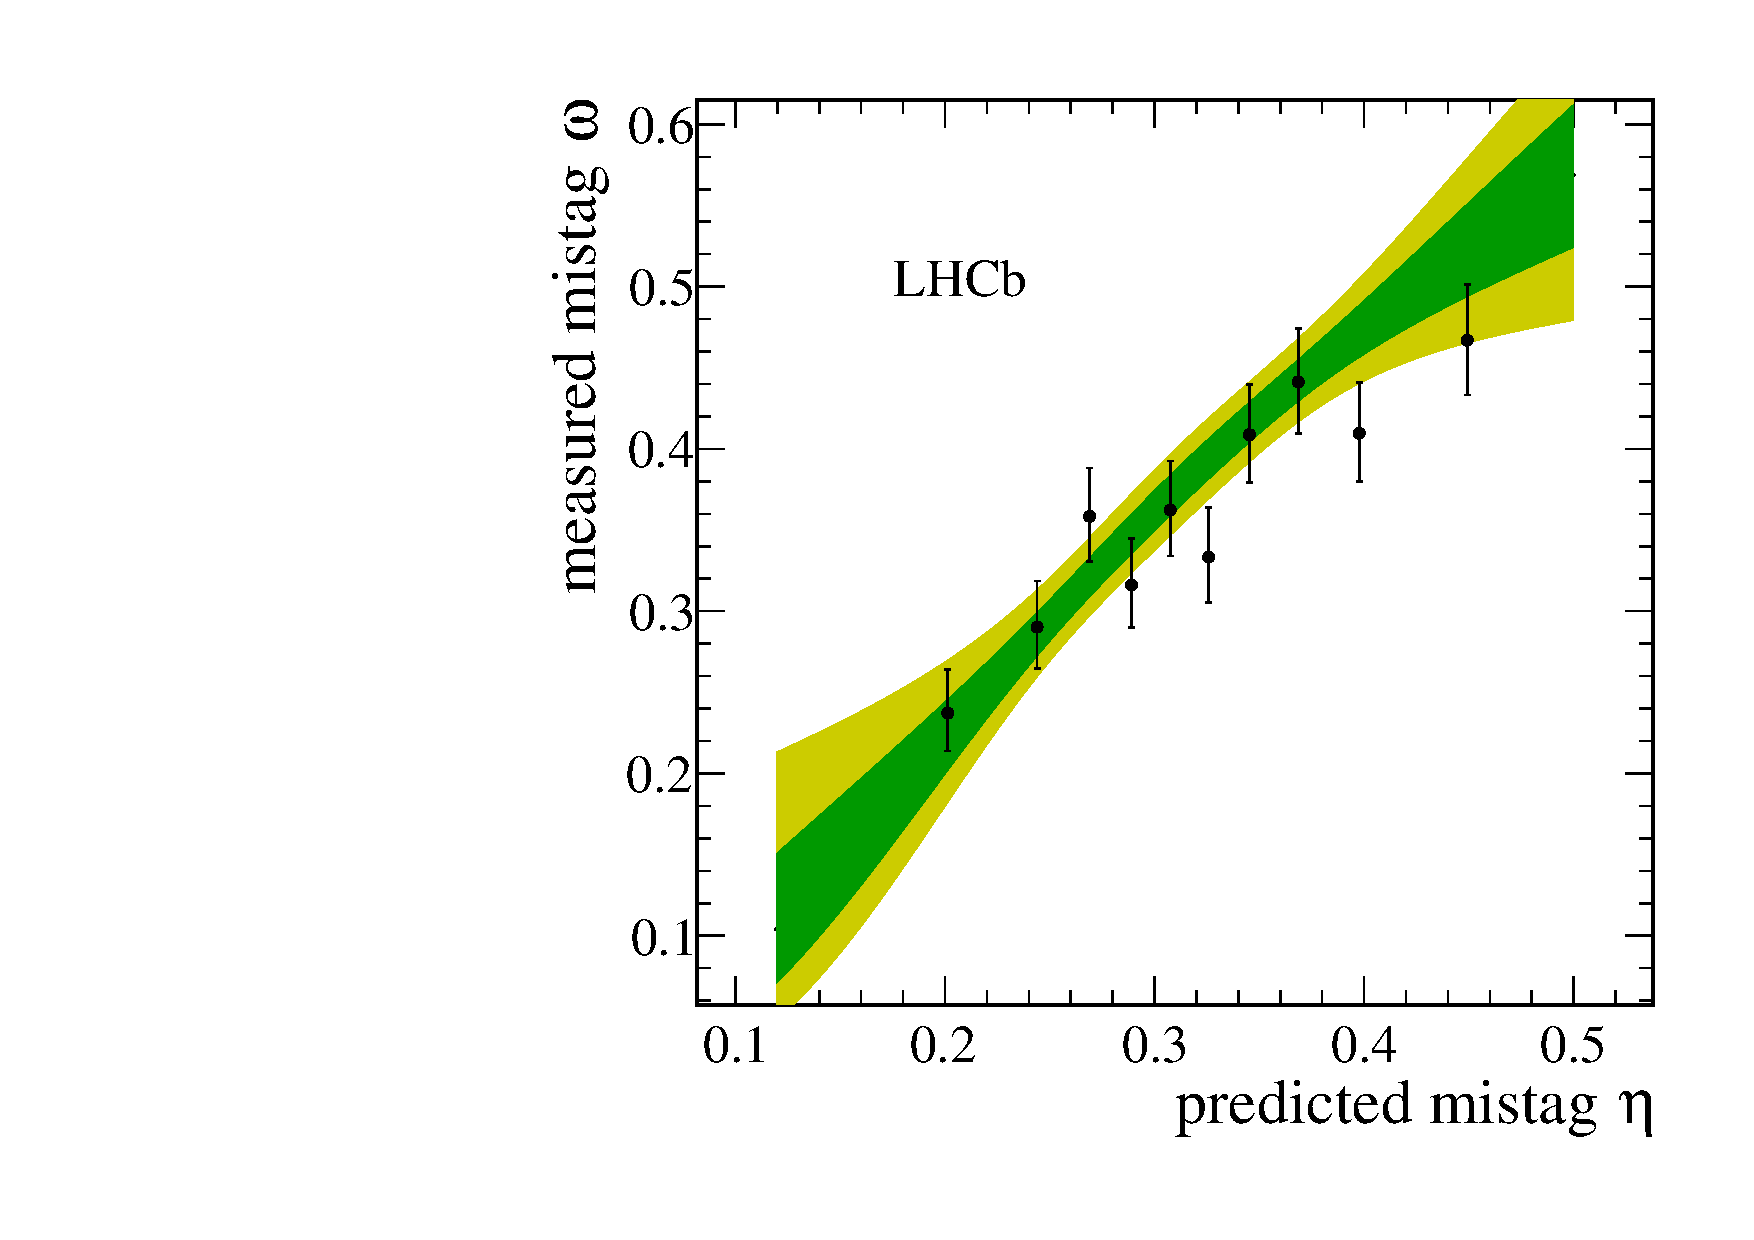
\includegraphics[width=0.26\textwidth]{04FlavourTagging/figs/OSelectronOpt/run1_tunings/OS_Electron_InputCalibration.pdf}
  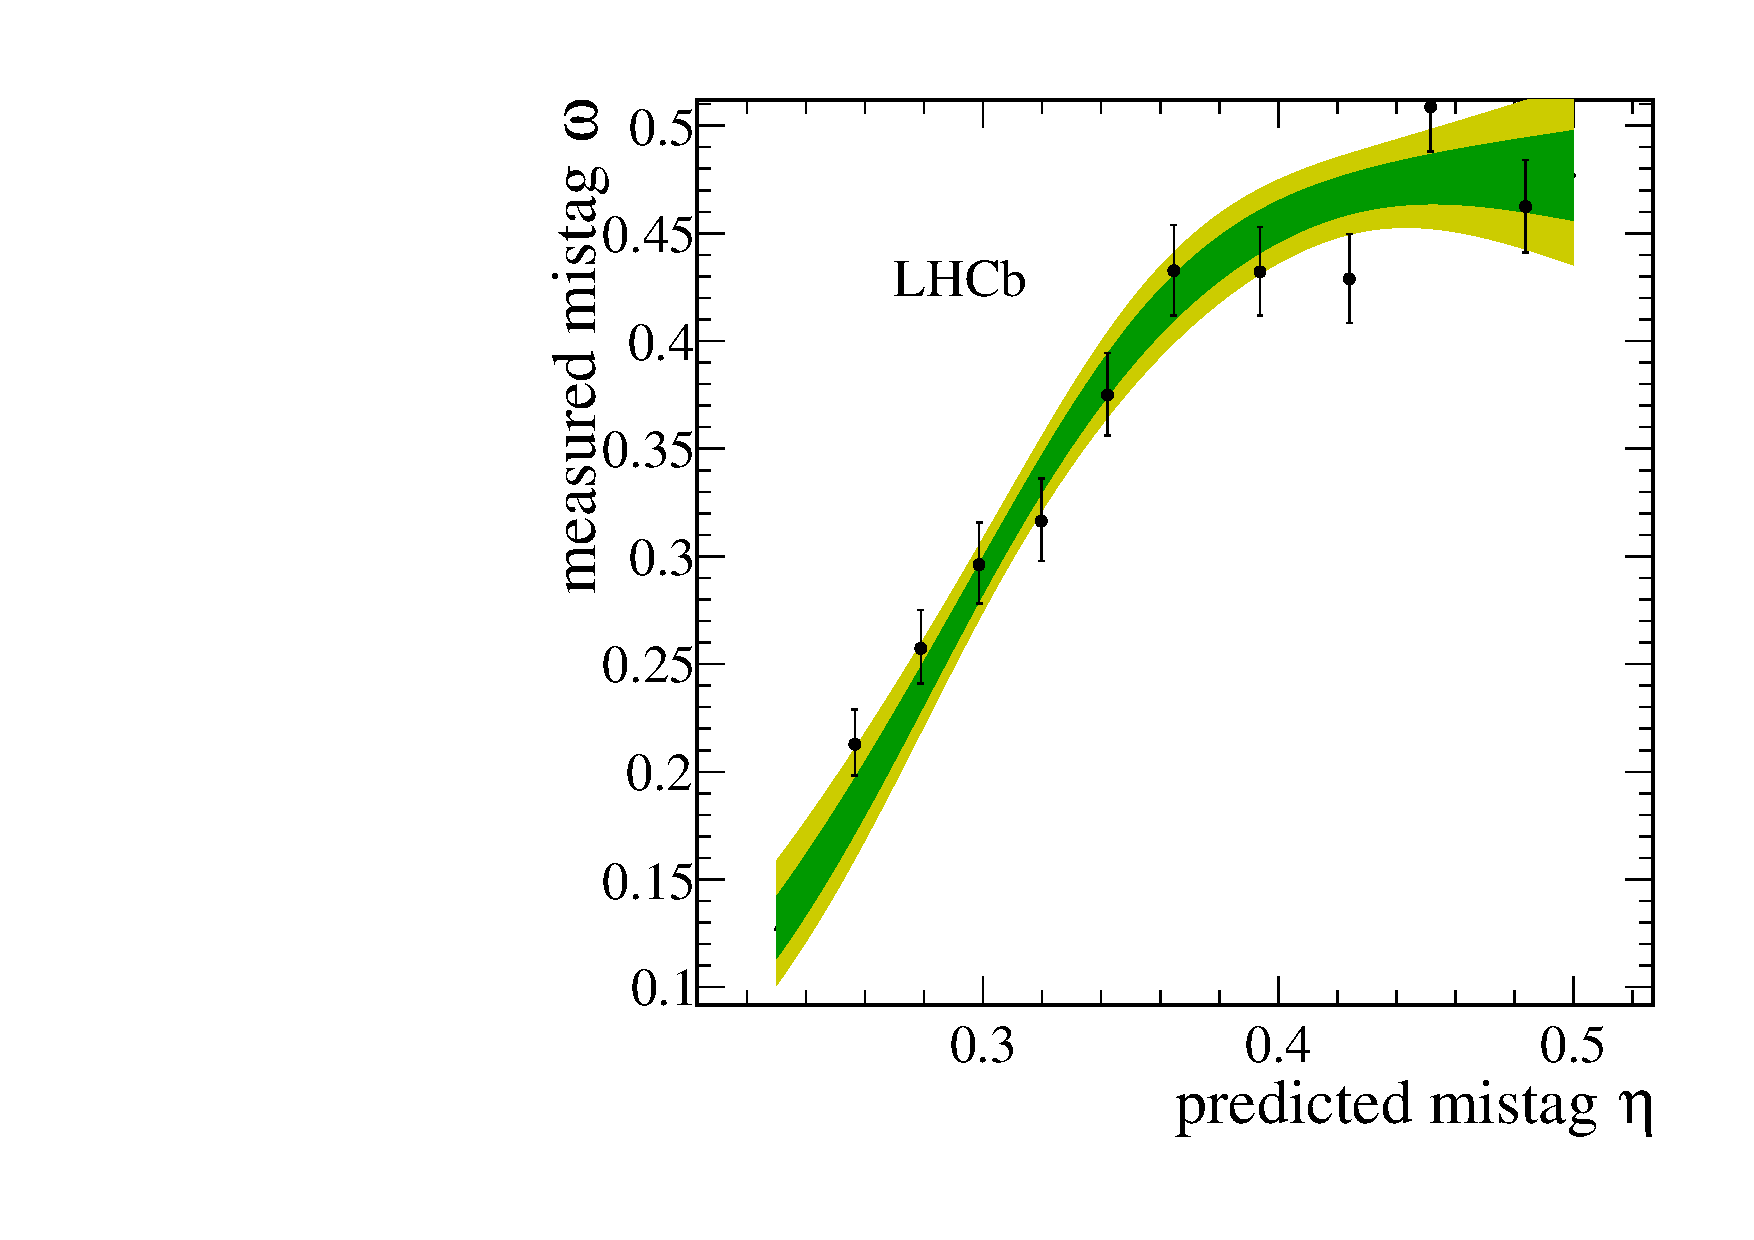
\includegraphics[width=0.26\textwidth]{04FlavourTagging/figs/OSelectronOpt/run2b2cc_tunings/OS_Electron_InputCalibration.pdf}
  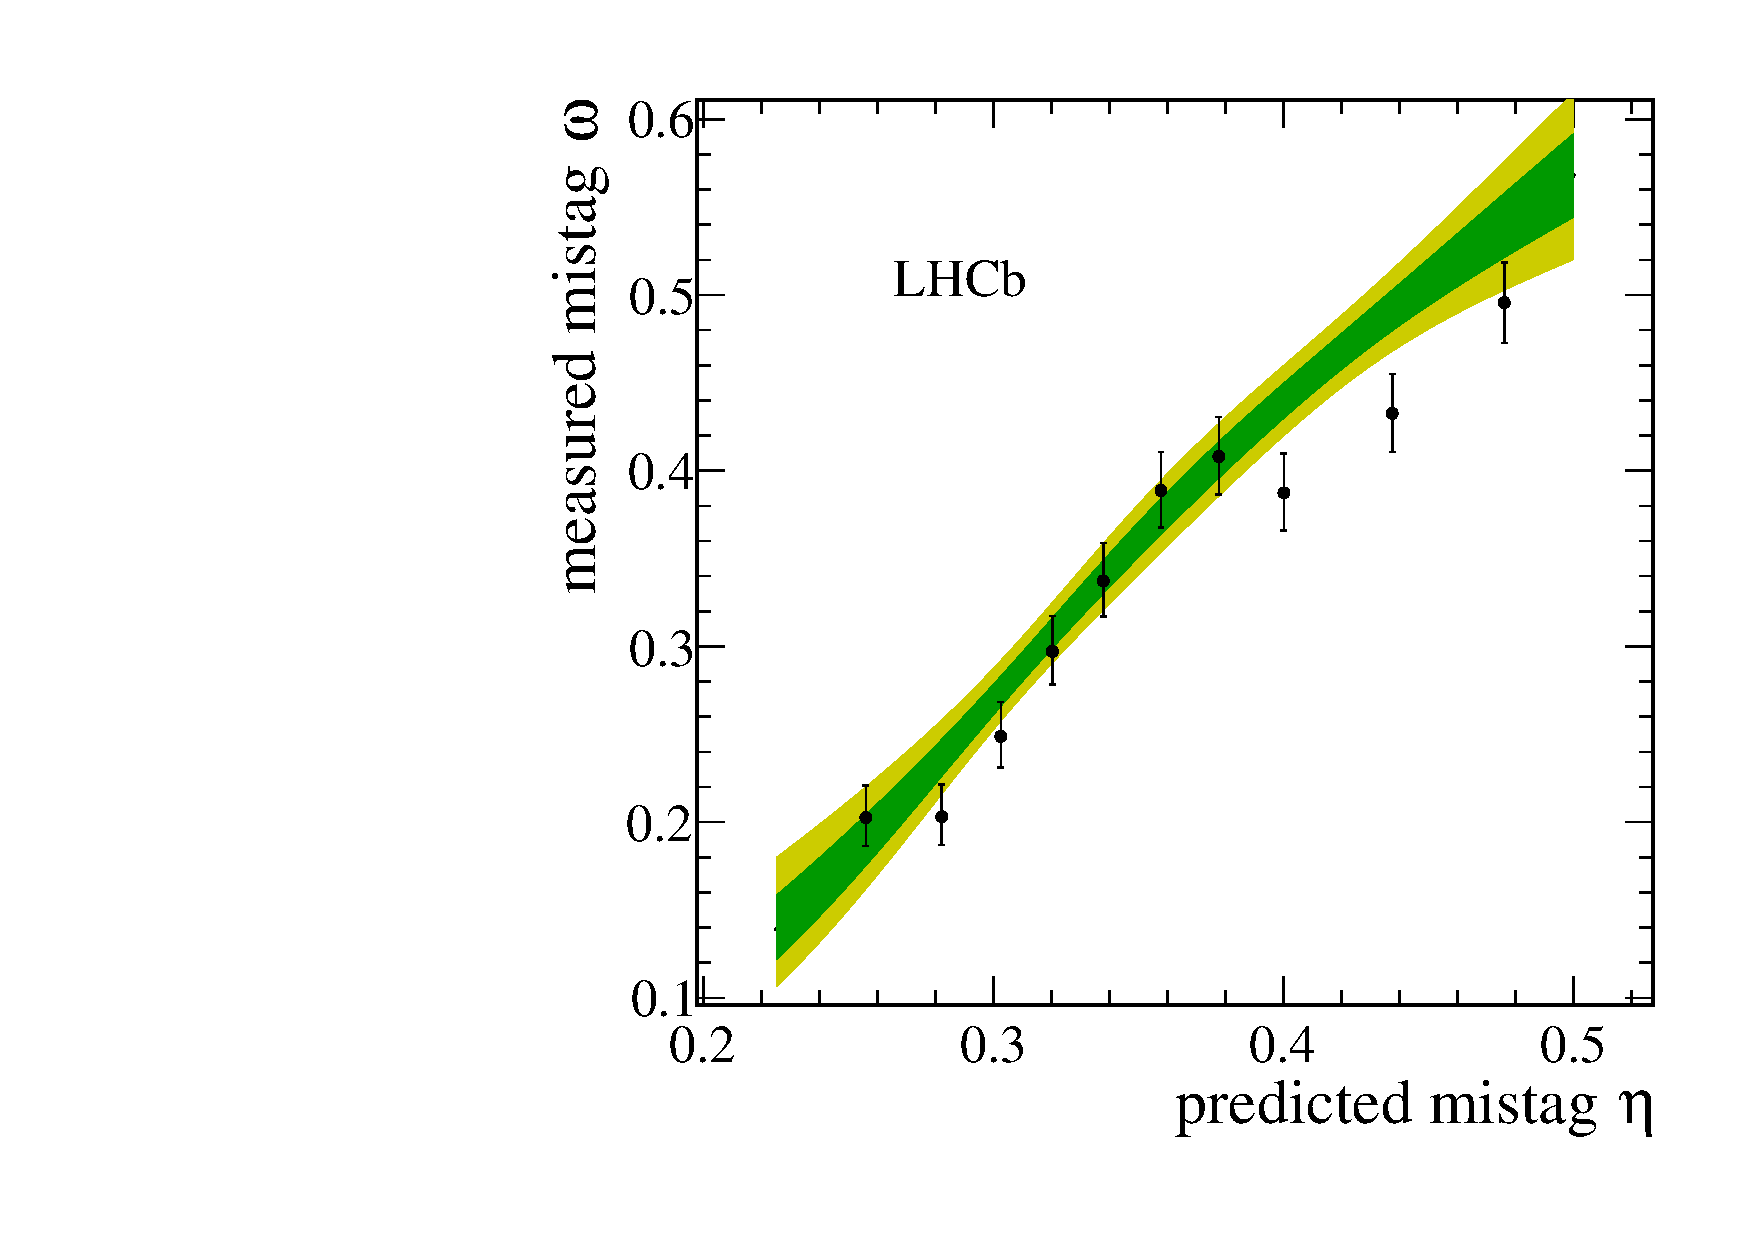
\includegraphics[width=0.26\textwidth]{04FlavourTagging/figs/OSelectronOpt/run2b2oc_tunings/OS_Electron_InputCalibration.pdf} \\
  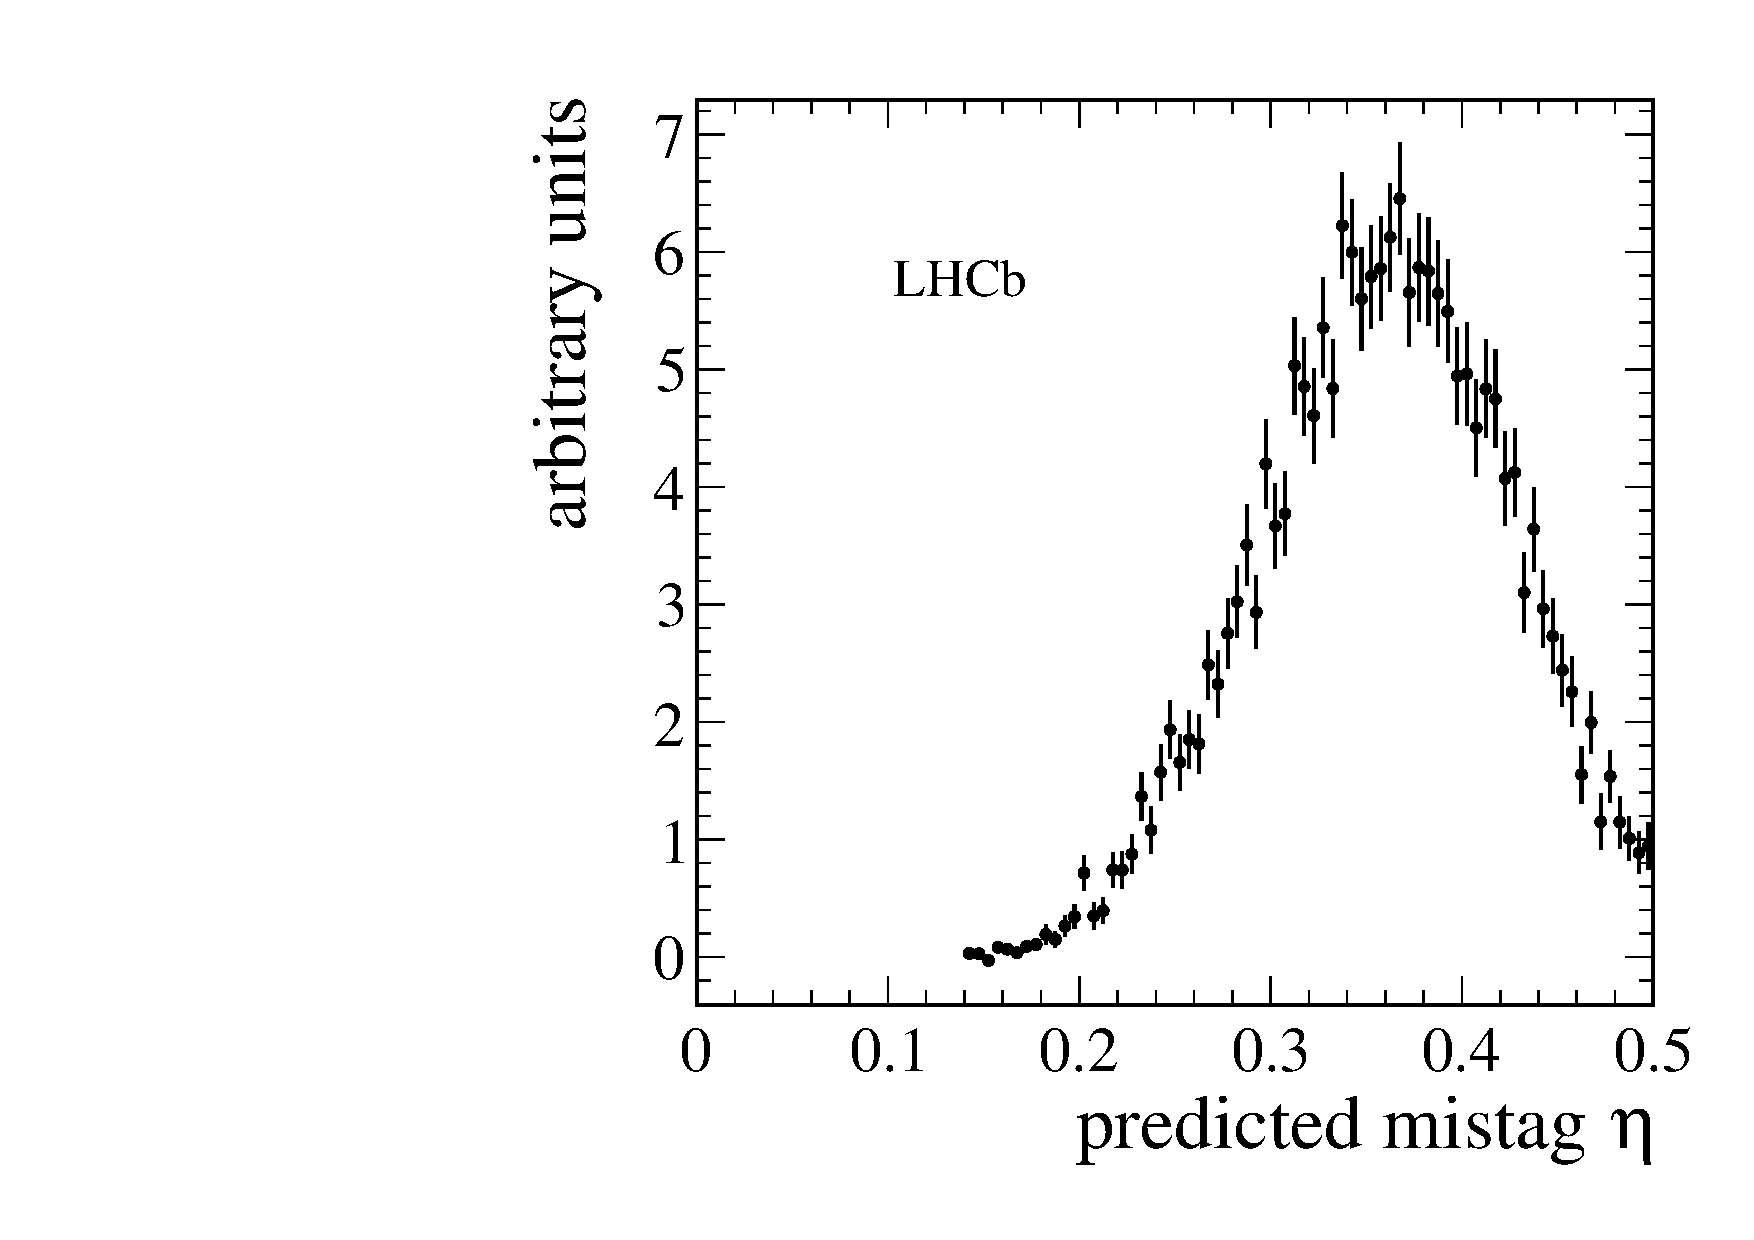
\includegraphics[width=0.26\textwidth]{04FlavourTagging/figs/OSelectronOpt/run1_tunings/OS_Electron_EtaDist.pdf}
  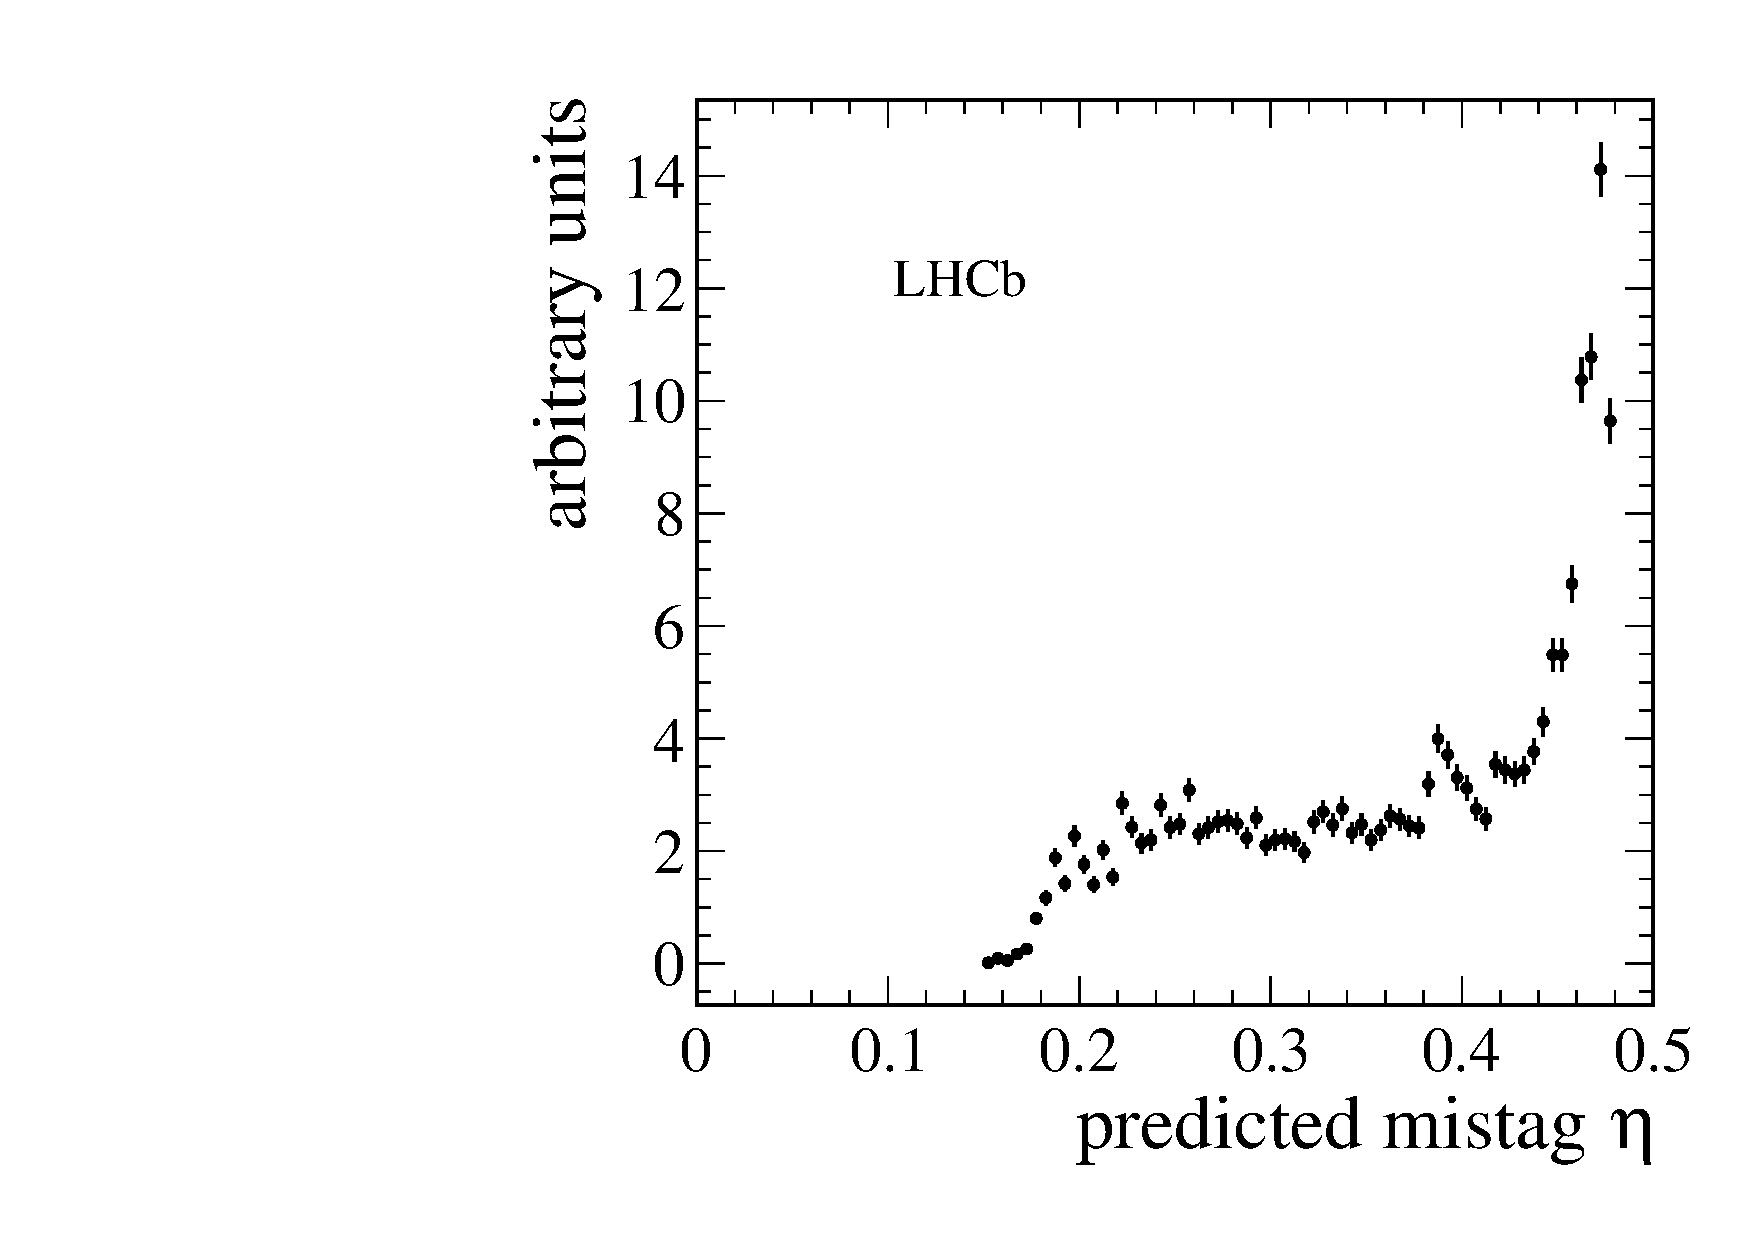
\includegraphics[width=0.26\textwidth]{04FlavourTagging/figs/OSelectronOpt/run2b2cc_tunings/OS_Electron_EtaDist.pdf}
  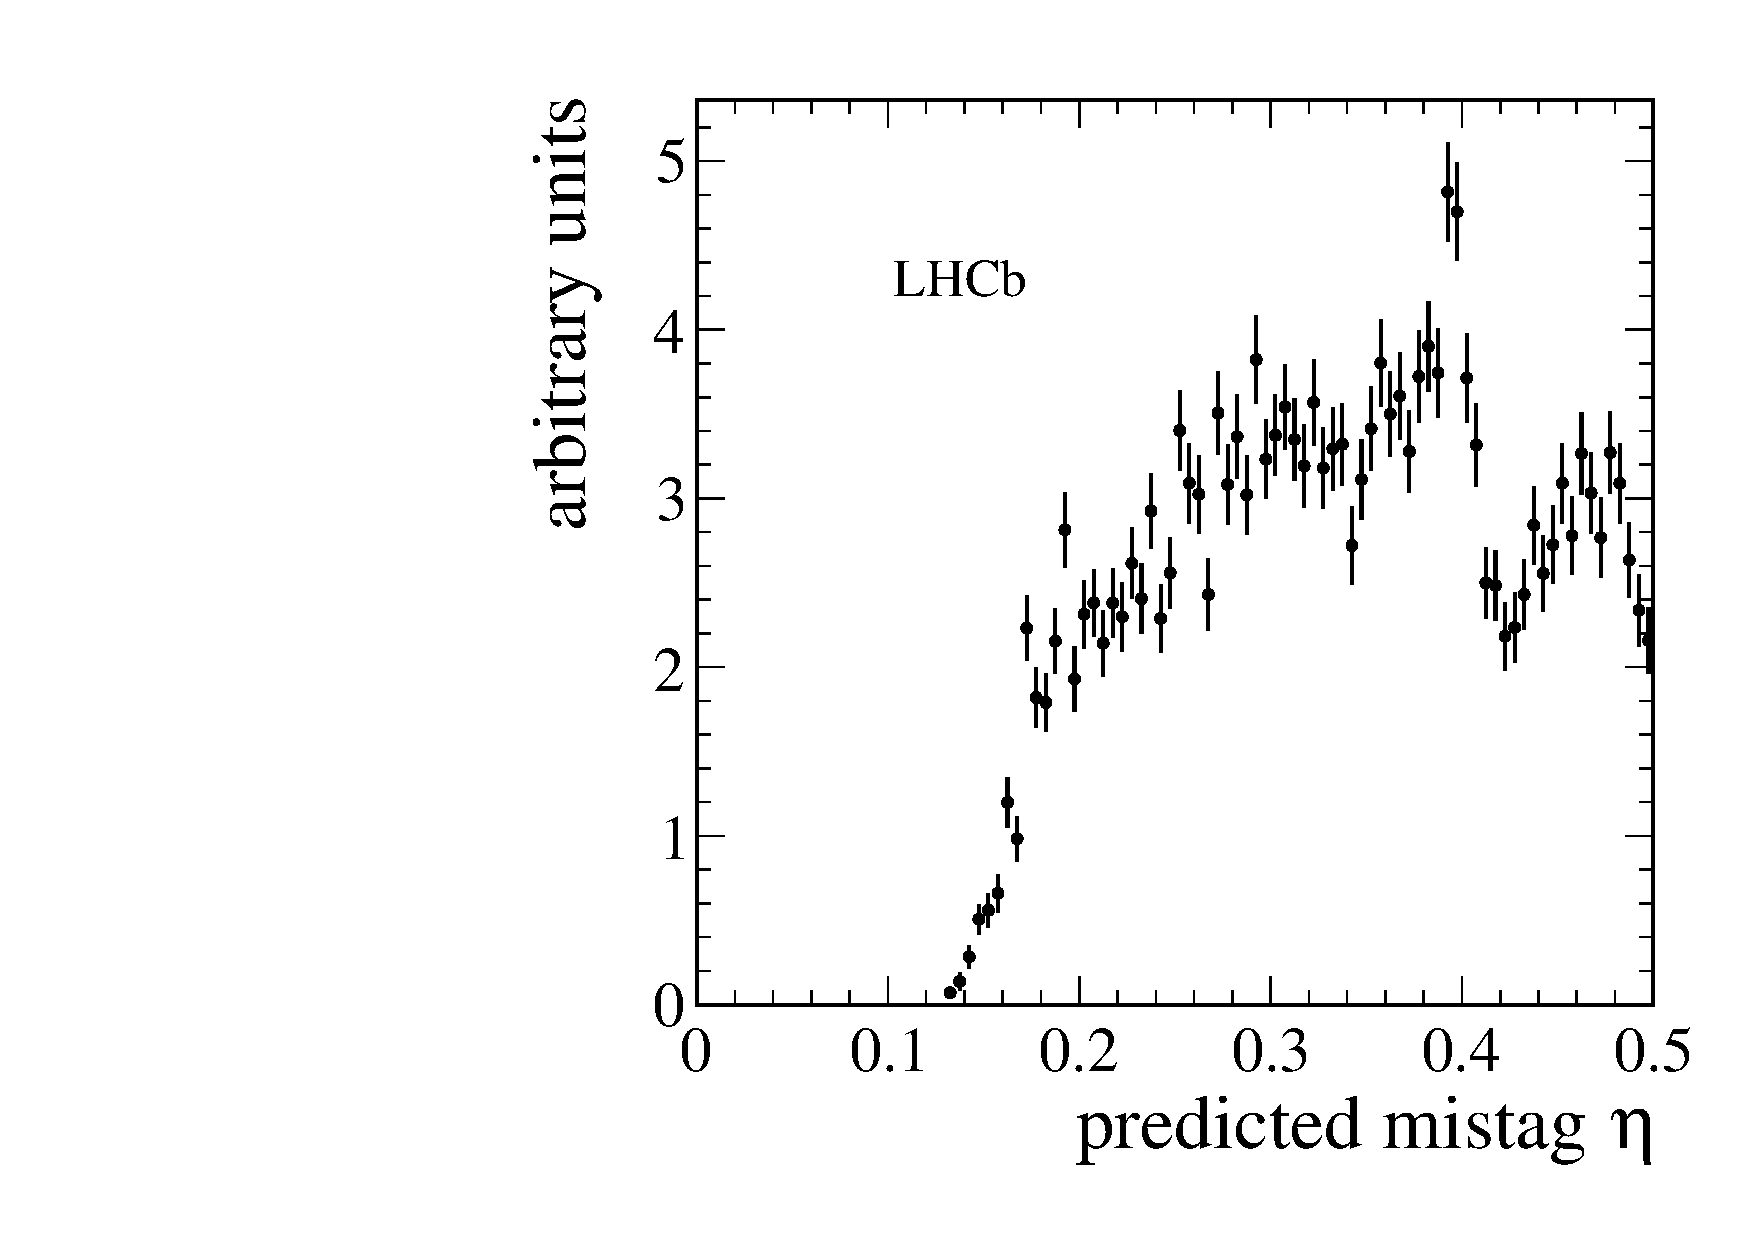
\includegraphics[width=0.26\textwidth]{04FlavourTagging/figs/OSelectronOpt/run2b2oc_tunings/OS_Electron_EtaDist.pdf}
  \caption{Mistag calibration results on \emph{sWeighted} Run 2 $B^0\to D^-\pi^+$ data for the \OSe~taggers. The results obtained with the Run 1 old (left), Run 2 B2CC (center), and Run 2 B2OC (right) tunings are shown.
The \emph{sWeighted} data sample is shown as black points. The green (yellow) band indicates the 68\% (95\%) C.L. interval for the fitted calibration functions. Bottom: distributions of the uncalibrated mistag $\eta$.}
  \label{fig:OSePerfCalib3}
\end{figure}


\begin{figure}[ht!]
  \centering
  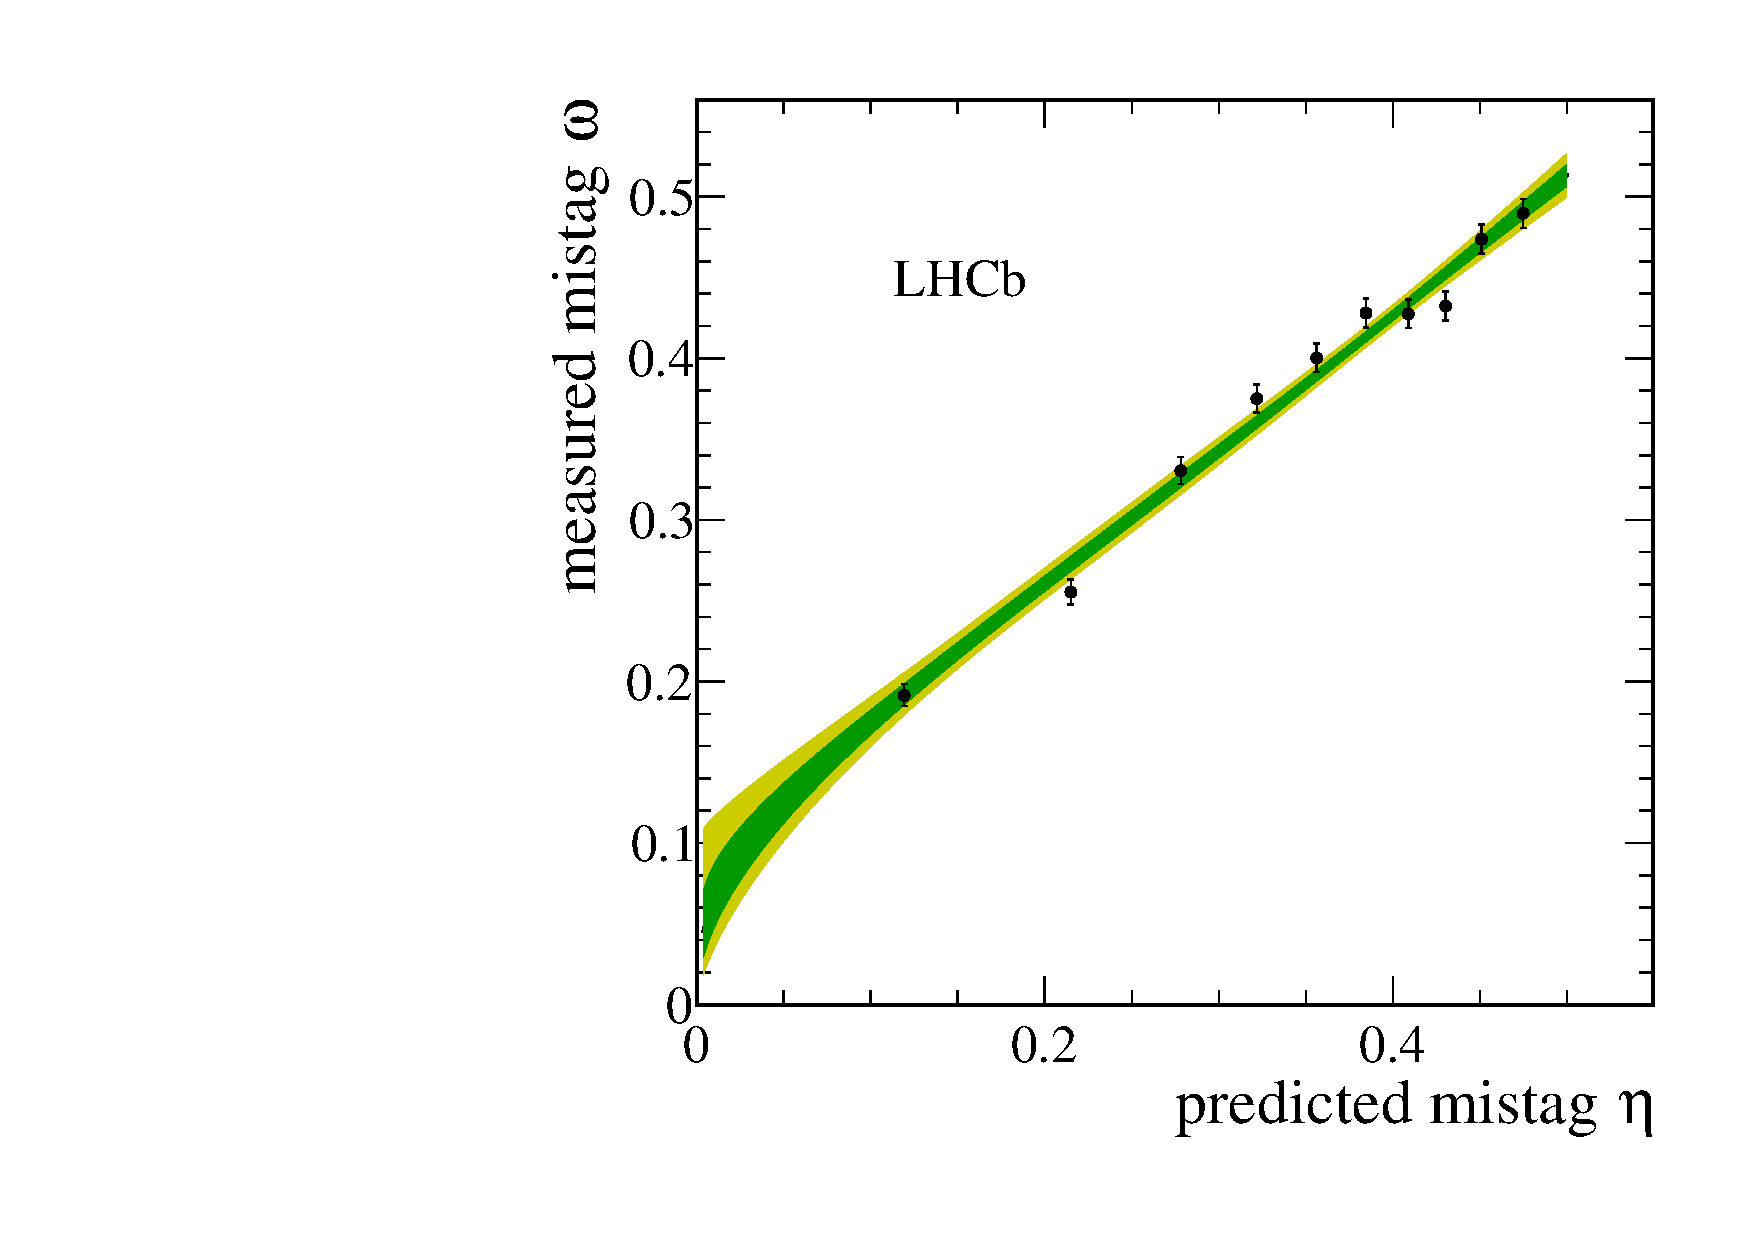
\includegraphics[width=0.26\textwidth]{04FlavourTagging/figs/OSelectronOpt/run1data_old/OS_Combination_Calibration.pdf}
  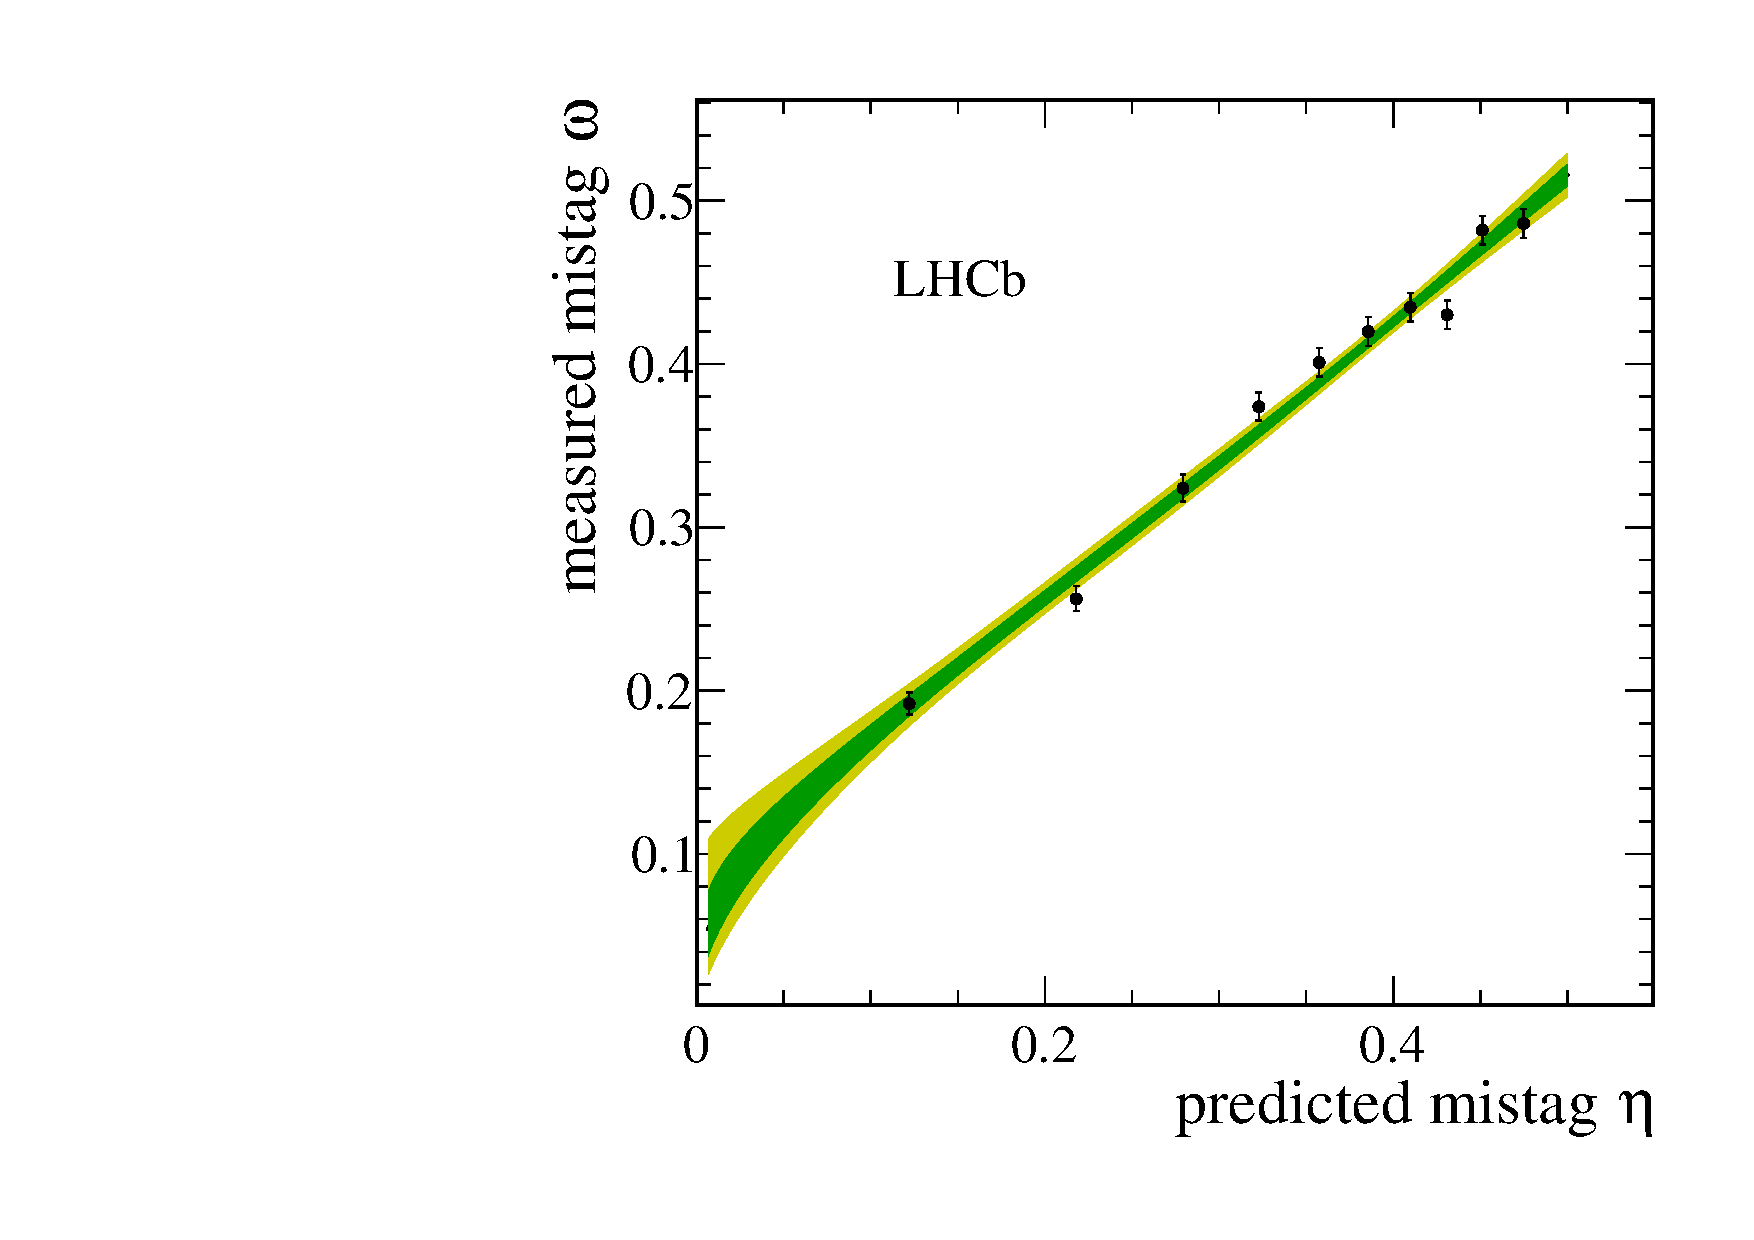
\includegraphics[width=0.26\textwidth]{04FlavourTagging/figs/OSelectronOpt/run1data_new/OS_Combination_Calibration.pdf} \\
  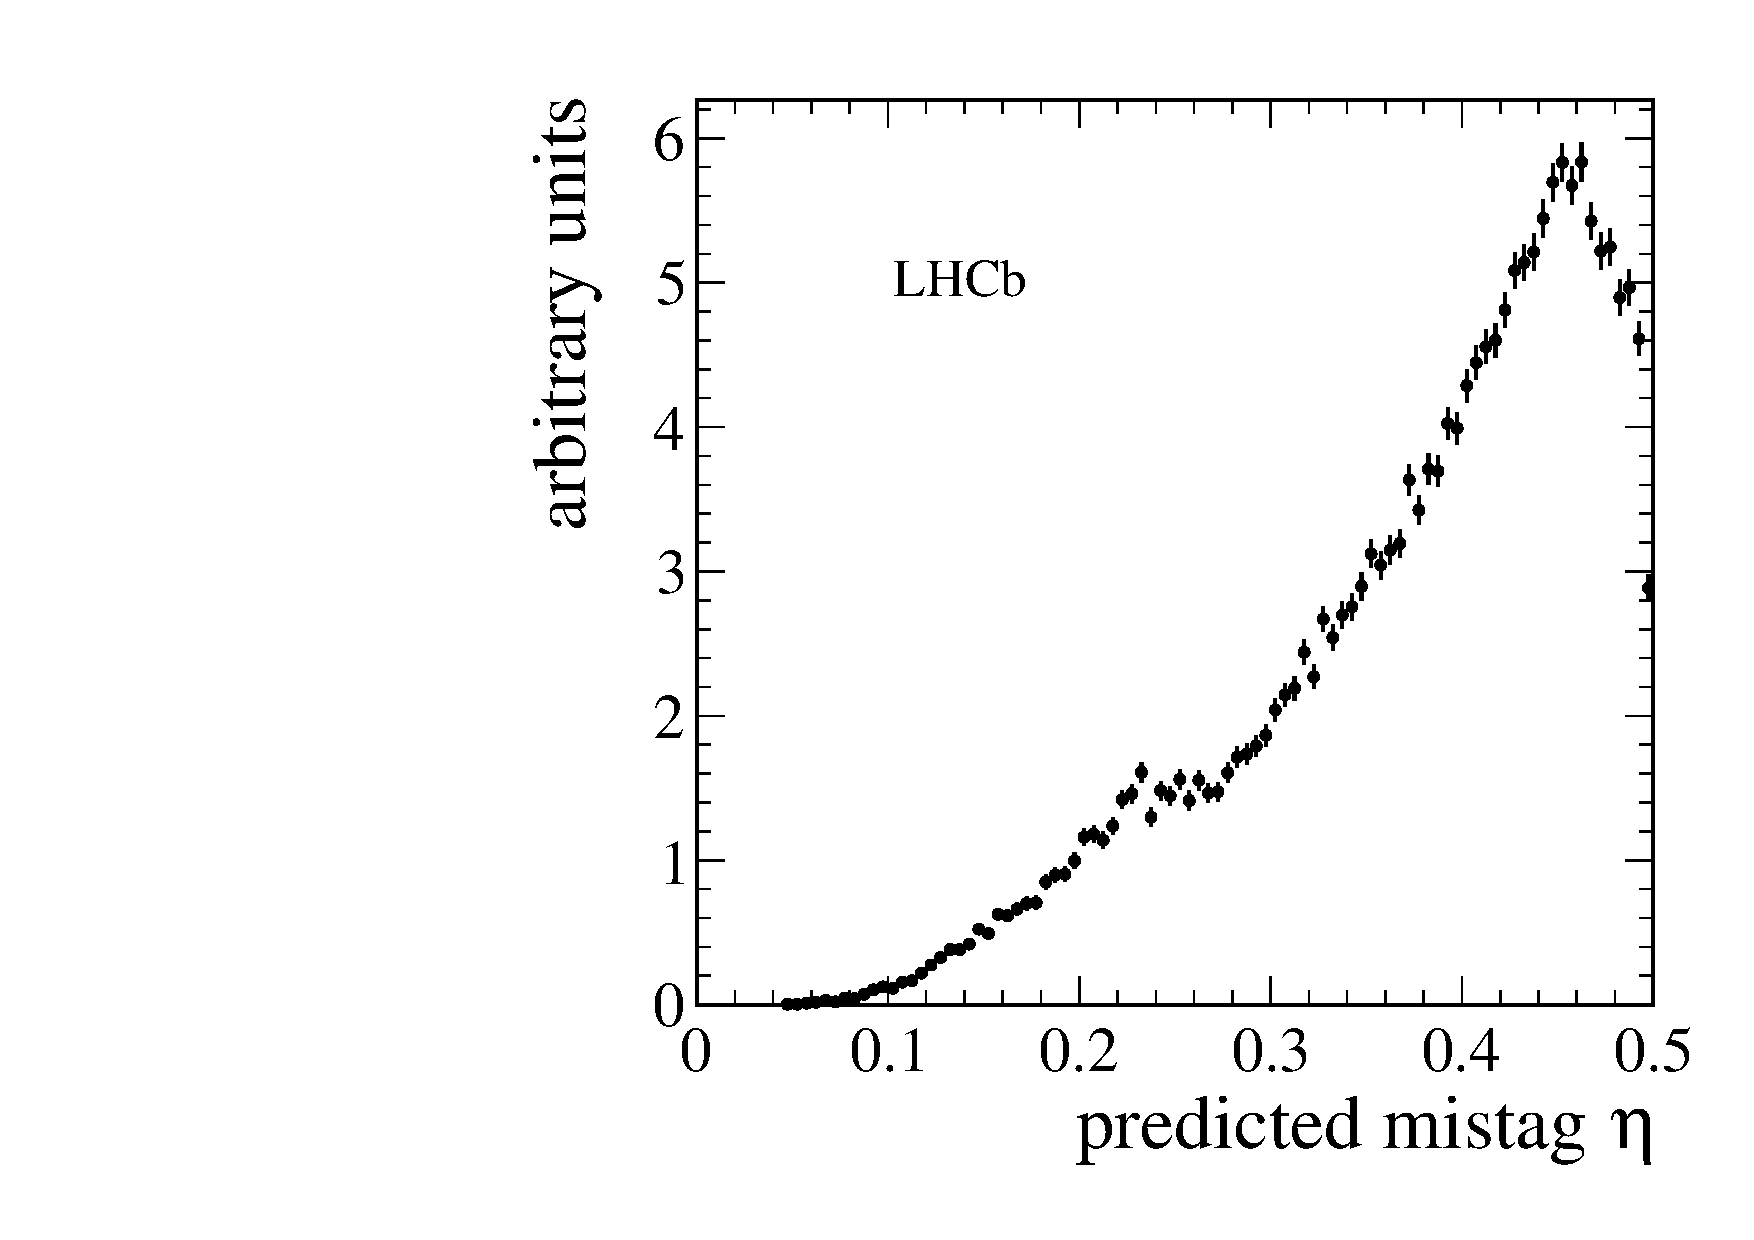
\includegraphics[width=0.26\textwidth]{04FlavourTagging/figs/OSelectronOpt/run1data_old/OS_Combination_EtaDist.pdf}
  \includegraphics[width=0.26\textwidth]{04FlavourTagging/figs/OSelectronOpt/run1data_new/OS_Combination_EtaDist.pdf} 
  \vspace{-2mm}
  \caption{Top: mistag calibration results on \emph{sWeighted} Run 1 $B^0\to D^-\pi^+$ data for the combination of the OS taggers. The results obtained with the Run 1 old (left) and Run 1 new (right) tunings of \OSe~are shown. The \emph{sWeighted} data sample is shown as black points. The green (yellow) band indicates the 68\% (95\%) C.L. interval for the fitted calibration functions. Bottom: distributions of the uncalibrated mistag $\eta$.}
  \label{fig:OSePerfCalib2}
\end{figure}

\begin{figure}[hb!]
  \centering
  \includegraphics[width=0.26\textwidth]{04FlavourTagging/figs/OSelectronOpt/run1_tunings/OS_Combination_Calibration.pdf}
  \includegraphics[width=0.26\textwidth]{04FlavourTagging/figs/OSelectronOpt/run2b2cc_tunings/OS_Combination_Calibration.pdf}
  \includegraphics[width=0.26\textwidth]{04FlavourTagging/figs/OSelectronOpt/run2b2oc_tunings/OS_Combination_Calibration.pdf} \\
  \includegraphics[width=0.26\textwidth]{04FlavourTagging/figs/OSelectronOpt/run1_tunings/OS_Combination_EtaDist.pdf}
  \includegraphics[width=0.26\textwidth]{04FlavourTagging/figs/OSelectronOpt/run2b2cc_tunings/OS_Combination_EtaDist.pdf}
  \includegraphics[width=0.26\textwidth]{04FlavourTagging/figs/OSelectronOpt/run2b2oc_tunings/OS_Combination_EtaDist.pdf}
  \vspace{-2mm}
  \caption{Mistag calibration results on \emph{sWeighted} Run 2 $B^0\to D^-\pi^+$ data for the combination of the OS taggers. The results obtained with the Run 1 old (left), Run 2 B2CC (center), and Run 2 B2OC (right) tunings of \OSe, \OSmu, and \OSK~are shown. The \emph{sWeighted} data sample is shown as black points. The green (yellow) band indicates the 68\% (95\%) C.L. interval for the fitted calibration functions. Bottom: distributions of the uncalibrated mistag $\eta$.}
  \label{fig:OSePerfCalib4}
\end{figure}

The performance is reported in Tables~\ref{tab:Bd2DpiperformanceRun1}~and~\ref{tab:Bd2DpiperformanceRun2}.
The Run 1 new tuning allows to gain a relative $~9\%$ in tagging power for the \OSe~tagger on Run 1 data; the corresponding, relative gain of the OS combination is $~3\%$.
The tagging power of \OSvtx~and \OSc, which were trained on Run 1 data, increases on Run 2 data compared to Run 1; 
for this reason, no specific optimisation for the Run 2 conditions is performed.
The tagging power of \OSe, \OSmu, and \OSK~with the Run 1 tunings is lower on Run 2 data compared to Run 1. 
However, compared to the Run 1 tunings, the Run 2 tunings show a relative improvement in tagging power of about $\sim 160\%$ for \OSe, and $\sim 6\%$ for \OSmu~and \OSK~on Run 2 data. This allows to recover similar performances as the ones obtained on Run 1 data with the Run 1 tunings, both for the individual taggers and their combination.
Moreover, the Run 2 B2CC and B2OC tunings show consistent tagging powers on Run 2 data, meaning that the optimisation is robust against the different kinematics of the adopted decays.

\begin{table}
\centering
\caption{Performance (tagging efficiency, average mistag and tagging power in $\%$) of the OS taggers on \emph{sWeighted} Run 1 $B^0\to D^-\pi^+$ data. The numbers for \OSe~and the OS combination are shown separately for the Run 1 old and Run 1 new tunings. The first uncertainty is statistical and the second comes from the calibration.}
\label{tab:Bd2DpiperformanceRun1}
%\resizebox{\textwidth}{!}{
\begin{tabular*}{\textwidth}{rlllll}
\toprule
\multicolumn{1}{c}{Tagger} & \multicolumn{1}{c}{$\etag$} & \multicolumn{1}{c}{$\avg{\mistag}$} & \multicolumn{1}{c}{$\effeff$} \\
\midrule
\OSvtx& $22.026\pm0.100$& $37.295\pm0.030\pm0.376$& $1.422\pm0.009\pm0.084$\\
\OSc& $4.632\pm0.050$& $34.026\pm0.049\pm0.824$& $0.473\pm0.006\pm0.049$\\
\hline
\OSe~Run 1 old& $3.028\pm0.041$& $30.570\pm0.113\pm0.963$& $0.457\pm0.008\pm0.045$\\
\OSe~Run 1 new& $4.337\pm0.049$& $33.089\pm0.085\pm0.777$& $0.496\pm0.007\pm0.046$\\
\hline
\OSmu~Run 1& $8.539\pm0.067$& $28.756\pm0.071\pm0.582$& $1.541\pm0.016\pm0.085$\\
\hline
\OSK~Run 1& $18.800\pm0.094$& $36.724\pm0.031\pm0.417$& $1.325\pm0.009\pm0.083$\\
\hline
\begin{tabular}{c} OS combination \\ Run 1 old \end{tabular}& $39.004\pm0.117$& $34.679\pm0.035\pm0.273$& $3.662\pm0.020\pm0.131$\\
\begin{tabular}{c} OS combination \\ Run 1 new \end{tabular}& $39.733\pm0.118$& $34.576\pm0.035\pm0.270$& $3.781\pm0.021\pm0.133$\\
\bottomrule
\end{tabular*}
%}
\end{table}

\begin{table}
\centering
\caption{Performance (tagging efficiency, average mistag and tagging power in $\%$) of the OS taggers on \emph{sWeighted} Run 2 $B^0\to D^-\pi^+$ data. The numbers for \OSe, \OSmu, \OSK, and the OS combination are shown separately for the Run 1, Run 2 B2CC, and Run 2 B2OC tunings. The first uncertainty is statistical and the second comes from the calibration.}
\label{tab:Bd2DpiperformanceRun2}
%\resizebox{\textwidth}{!}{
\begin{tabular*}{\textwidth}{rlllll}
\toprule
\multicolumn{1}{c}{Tagger} & \multicolumn{1}{c}{$\etag$} & \multicolumn{1}{c}{$\avg{\mistag}$} & \multicolumn{1}{c}{$\effeff$} \\
\midrule
\OSvtx& $20.834\pm0.075$& $36.139\pm0.029\pm0.301$& $1.601\pm0.009\pm0.070$\\ 
\OSc& $5.025\pm0.040$& $33.875\pm0.041\pm0.624$& $0.523\pm0.005\pm0.040$\\
\hline
\OSe~Run 1 old& $1.868\pm0.025$& $34.300\pm0.096\pm0.941$& $0.184\pm0.003\pm0.022$\\
\OSe~Run 2 B2CC& $4.451\pm0.038$& $33.352\pm0.081\pm0.608$& $0.493\pm0.006\pm0.036$\\
\OSe~Run 2 B2OC& $3.333\pm0.033$& $30.917\pm0.075\pm0.702$& $0.486\pm0.006\pm0.036$\\
\hline
\OSmu~Run 1& $8.343\pm0.051$& $30.357\pm0.042\pm0.466$& $1.288\pm0.010\pm0.061$\\
\OSmu~Run 2 B2CC& $9.151\pm0.053$& $30.837\pm0.041\pm0.432$& $1.344\pm0.010\pm0.061$\\
\OSmu~Run 2 B2OC& $8.040\pm0.050$& $29.174\pm0.043\pm0.463$& $1.395\pm0.010\pm0.062$\\
\hline
\OSK~Run 1& $15.737\pm0.067$& $35.902\pm0.030\pm0.357$& $1.251\pm0.008\pm0.063$\\
\OSK~Run 2 B2CC& $19.516\pm0.073$& $36.889\pm0.026\pm0.310$& $1.342\pm0.007\pm0.064$\\
\OSK~Run 2 B2OC& $15.793\pm0.067$& $35.565\pm0.030\pm0.348$& $1.316\pm0.008\pm0.063$\\
\hline
\begin{tabular}{c} OS combination \\ Run 1 old \end{tabular}& $36.239\pm0.088$& $35.285\pm0.024\pm0.227$& $3.139\pm0.013\pm0.097$\\
\begin{tabular}{c} OS combination \\ Run 2 B2CC \end{tabular}& $40.154\pm0.090$& $35.123\pm0.025\pm0.210$& $3.555\pm0.014\pm0.100$\\
\begin{tabular}{c} OS combination \\ Run 2 B2OC \end{tabular}& $36.555\pm0.089$& $34.225\pm0.026\pm0.220$& $3.638\pm0.015\pm0.102$\\
\bottomrule
\end{tabular*}
%}
\end{table}

